\chapter{Contribution 2: Optimization of OCR Models }
\clearpage
\section{Introduction}
Optimizing OCR models is essential to improve their accuracy and efficiency, especially when dealing with complex and critical data such as medical labels. This chapter focuses on the optimization techniques used to enhance the performance of three OCR engines: Tesseract OCR, EasyOCR, and TrOCR.

We explore the process of fine-tuning these models using two optimization methods—Optuna, a modern hyperparameter tuning framework, and Genetic Algorithms, an evolutionary approach inspired by natural selection. These methods help identify the best settings for each model to reduce recognition errors and improve overall reliability.

The goal of this chapter is to present the applied optimization strategies, compare their impact on model performance, and highlight the most effective approaches for real-world OCR tasks in the medical field.

\vspace{-0.5cm}
\section{Optimization Definition}
Optimization is known as the act of choosing the optimal choice from a range of options, and it frequently aims to maximize predicted benefit. Optimization entails determining the option with the greatest potential benefit; yet, because of time restrictions, uncertainty, and partial information, this process can be computationally demanding and difficult in real-world decision-making. In reality, decision-makers frequently use "satisficing"—selecting the first feasible alternative instead of the best one. Depending on one's cognitive, behavioral, cultural, or evolutionary viewpoint, the term "optimization" can refer to both the quality of the result and the process employed to get there \cite{klein2001fiction}.
\vspace{-0.5cm}
\section{Strategies of optimization in ML/DL Models}
Optimization strategies in machine learning (ML) and deep learning (DL) models are crucial for improving model performance, accuracy, and efficiency. These strategies aim to minimize a loss function, which measures the discrepancy between the target values and the model's predictions. Gradient-based approaches like Stochastic Gradient Descent (SGD) and its more sophisticated variations, Adam, RMSprop, and Adagrad, are common optimization strategies that dynamically modify learning rates to improve convergence. In order to improve model behavior, hyperparameter tuning—which includes maximizing learning rates, batch sizes, and regularization strategies—is also essential. Additionally, advanced methods like early stopping, dropout, and data augmentation help prevent overfitting and improve generalization. Optimization techniques frequently extend to architectural decisions in the context of deep learning, including choosing the appropriate number of layers, neurons, and activation functions. When combined, these methods provide a solid basis for building ML/DL models that are effective on a variety of tasks and datasets.\cite{bian2024machine}
\vspace{-0.5cm}

\subsection{Data Processing}
Machine Learning (ML) and Deep Learning (DL) model optimization depends heavily on correct data pre-processing, because overall performance, and the real efficiency of models, and their training are immediately affected. By changing the raw data into a structured and clean format, preprocessing simplifies optimization through removing inconsistencies and noise. Several useful techniques use feature scaling to normalize particular data ranges. Other methods use data augmentation to assist models in generalizing better, in addition to data cleaning for fixing mistakes. For text recognition, with its rise toward greatness inside optical character recognition (OCR) systems, particular preprocessing techniques are used, such as adaptive thresholding, noise reduction, and picture normalization. These preprocessing ways function as one in order to increase optimization efficiency along with producing accurate and reliable models.\cite{kshetry2021image}

\vspace{-0.5cm}
\subsection{Features Engineering}
Feature engineering is a fundamental step in machine learning (ML) that changes basic, unorganized data into useful features, increasing a model’s capacity for creation of correct decisions. To thoroughly catch underlying patterns throughout all of the data, n order to better capture the underlying patterns in the data, this procedure entails choosing, developing, and adjusting variables. Careful feature engineering greatly improves model performance and additionally lowers computational complexity, producing far more effective machine learning (ML) and deep learning (DL) systems. 

Deep learning is known to optimize features automatically and chooses information of most importance for the model under analysis, so it plays a critical role. This is true in many situations where the input data is large in amount and demands important processing power.\cite{zheng2018feature}
\vspace{-0.5cm}
\subsection{Hyperparameter Optimization (HPO)}
Hyperparameter Optimization (HPO) is a truly critical process in machine learning (ML) and also deep learning (DL) that focuses intently on selecting the superior set of hyperparameters to maximize a model’s performance. Model parameters are learned directly from the data during training. Hyperparameters, unlike model parameters, govern the overall behavior in the training process, such as the learning rate, batch size, number of layers, or number of neurons inside a neural network. Proper tuning of these hyperparameters notably effects model accuracy, generalization, as well as training efficiency.\cite{feurer2019hyperparameter}
\vspace{-0.5cm}
\section{Methods and tools of HPO}
Hyperparameter optimization (HPO) involves a diverse and all-embracing set of methods targeted at efficiently identifying the best model configurations. Common methods are Bayesian Optimization, Genetic Algorithms (GA), and Particle Swarm Optimization (PSO), all furnishing special methods to explore hyperparameter space. Multiple strong tools are available for Hyperparameter Optimization, including Optuna, Ray, Scikit-learn’s GridSearchCV and RandomizedSearchCV, and irace. These tools automate and simplify the optimization process. In addition, they help improve model performance through systematically tuning hyperparameters with efficiency and precision.
\vspace{-0.5cm}
\subsection{Tools for HPO}
Several tools for HPO can be used, such as:
\vspace{-0.5cm}
\subsubsection{Optuna}
Optuna is a powerful and flexible open-source framework designed for efficient hyperparameter optimization in machine learning and deep learning models. It supports a wide range of adaptation techniques, including Bayesian optimization, Tree-structured Parzen Estimator (TPE), and grid search, which makes it compatible with various adaptation requirements. The major features of Optuna include the ability to handle both disconnected and constant hyperparameters, the pruning mechanisms that quickly prevent trials to save time, and its visualization tool to track and analyze optimization results. With its simple and spontaneous python API, Optuna Tuning Complex has become a popular option for ML and DL models, balancing efficiency and ease of use \cite{akiba2019optuna}.
%add the logo of optuna
%add the key concepts as a flow chart for optuna's process
\begin{figure}[H]
    \centering
    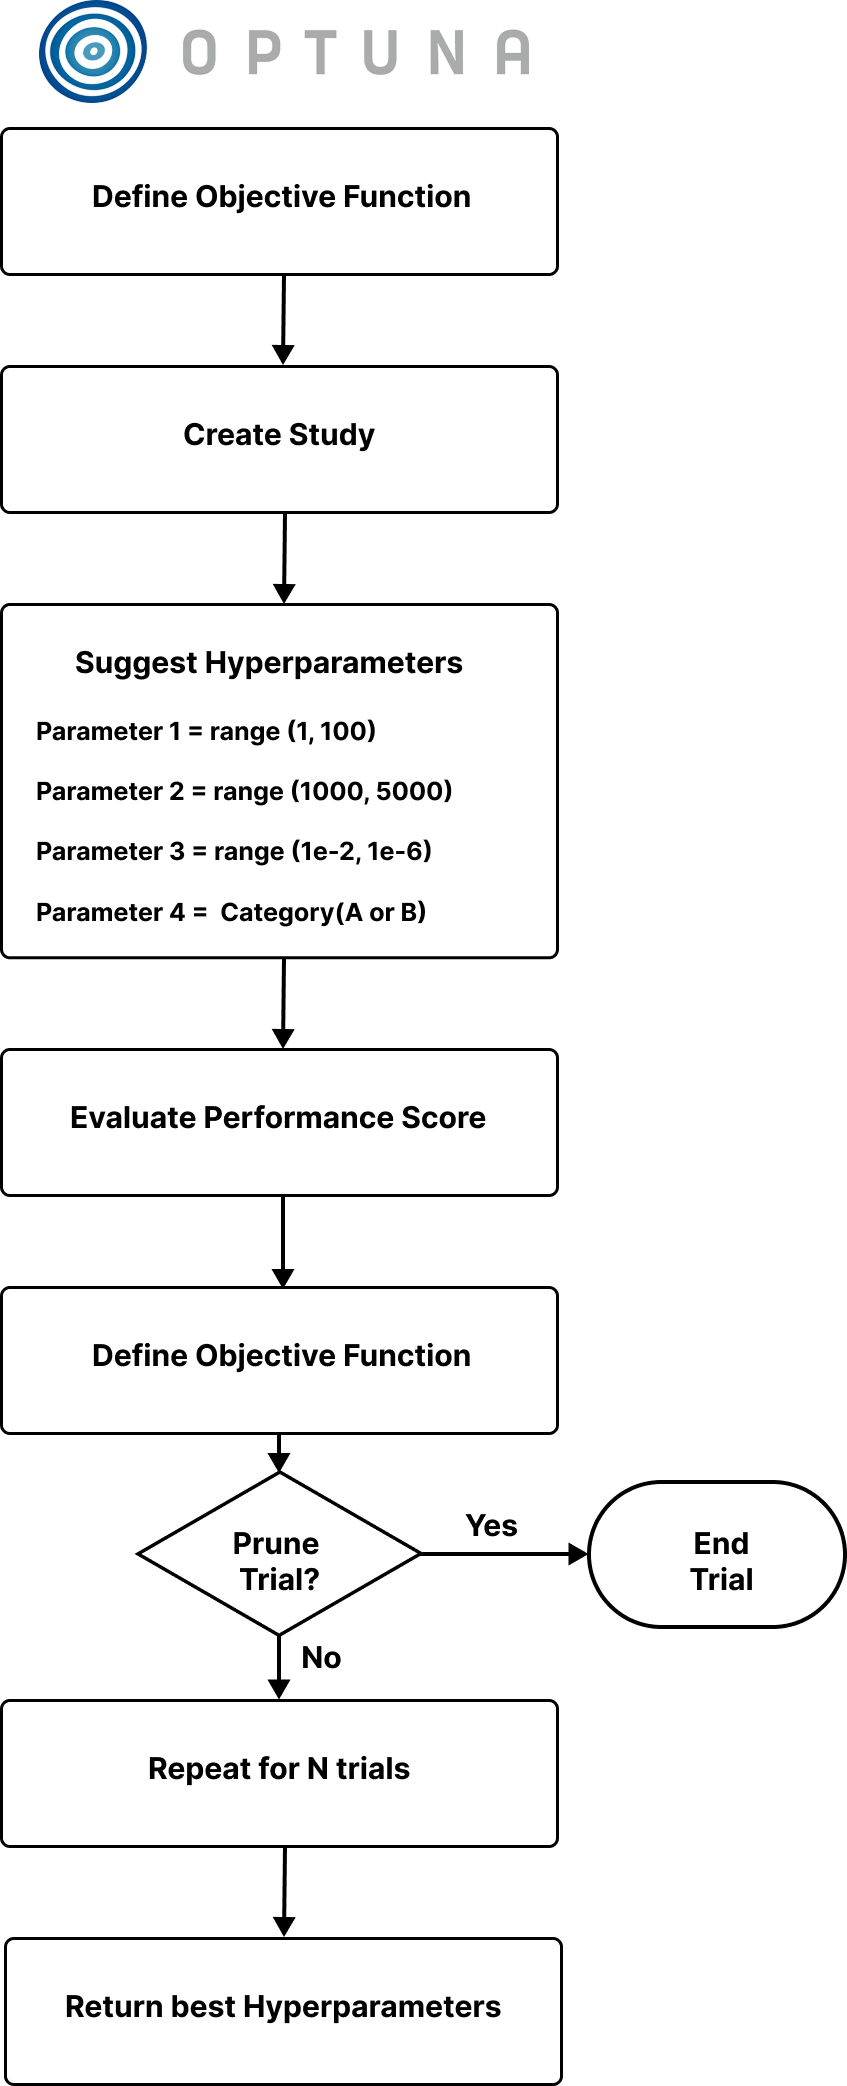
\includegraphics[width=8cm, height=14cm]{Figures/Chapter 4/optuna_process_flowchart.png}
    \caption{Optuna process flowchart}
    \label{fig:optunaprocessflowchart}
\end{figure}

\subsubsection{Ray}
Ray is an open-source unified framework for scaling AI and Python applications, specializing in machine learning (ML). It is an advanced compute layer for parallel processing that removes the requirement of expertise in distributed systems, and abstracts the complexity of executing individual and end-to-end ML workflows. Ray provides strong compute abstractions for building scalable platforms and a unified ML API for integrating easily within the ML ecosystem for ML platform builders and engineers. The friction between development and production is made small, as Ray allows the same Python code to span from a laptop to a massive cluster \cite{liaw2018tune}.


\begin{figure}[H]
    \centering
    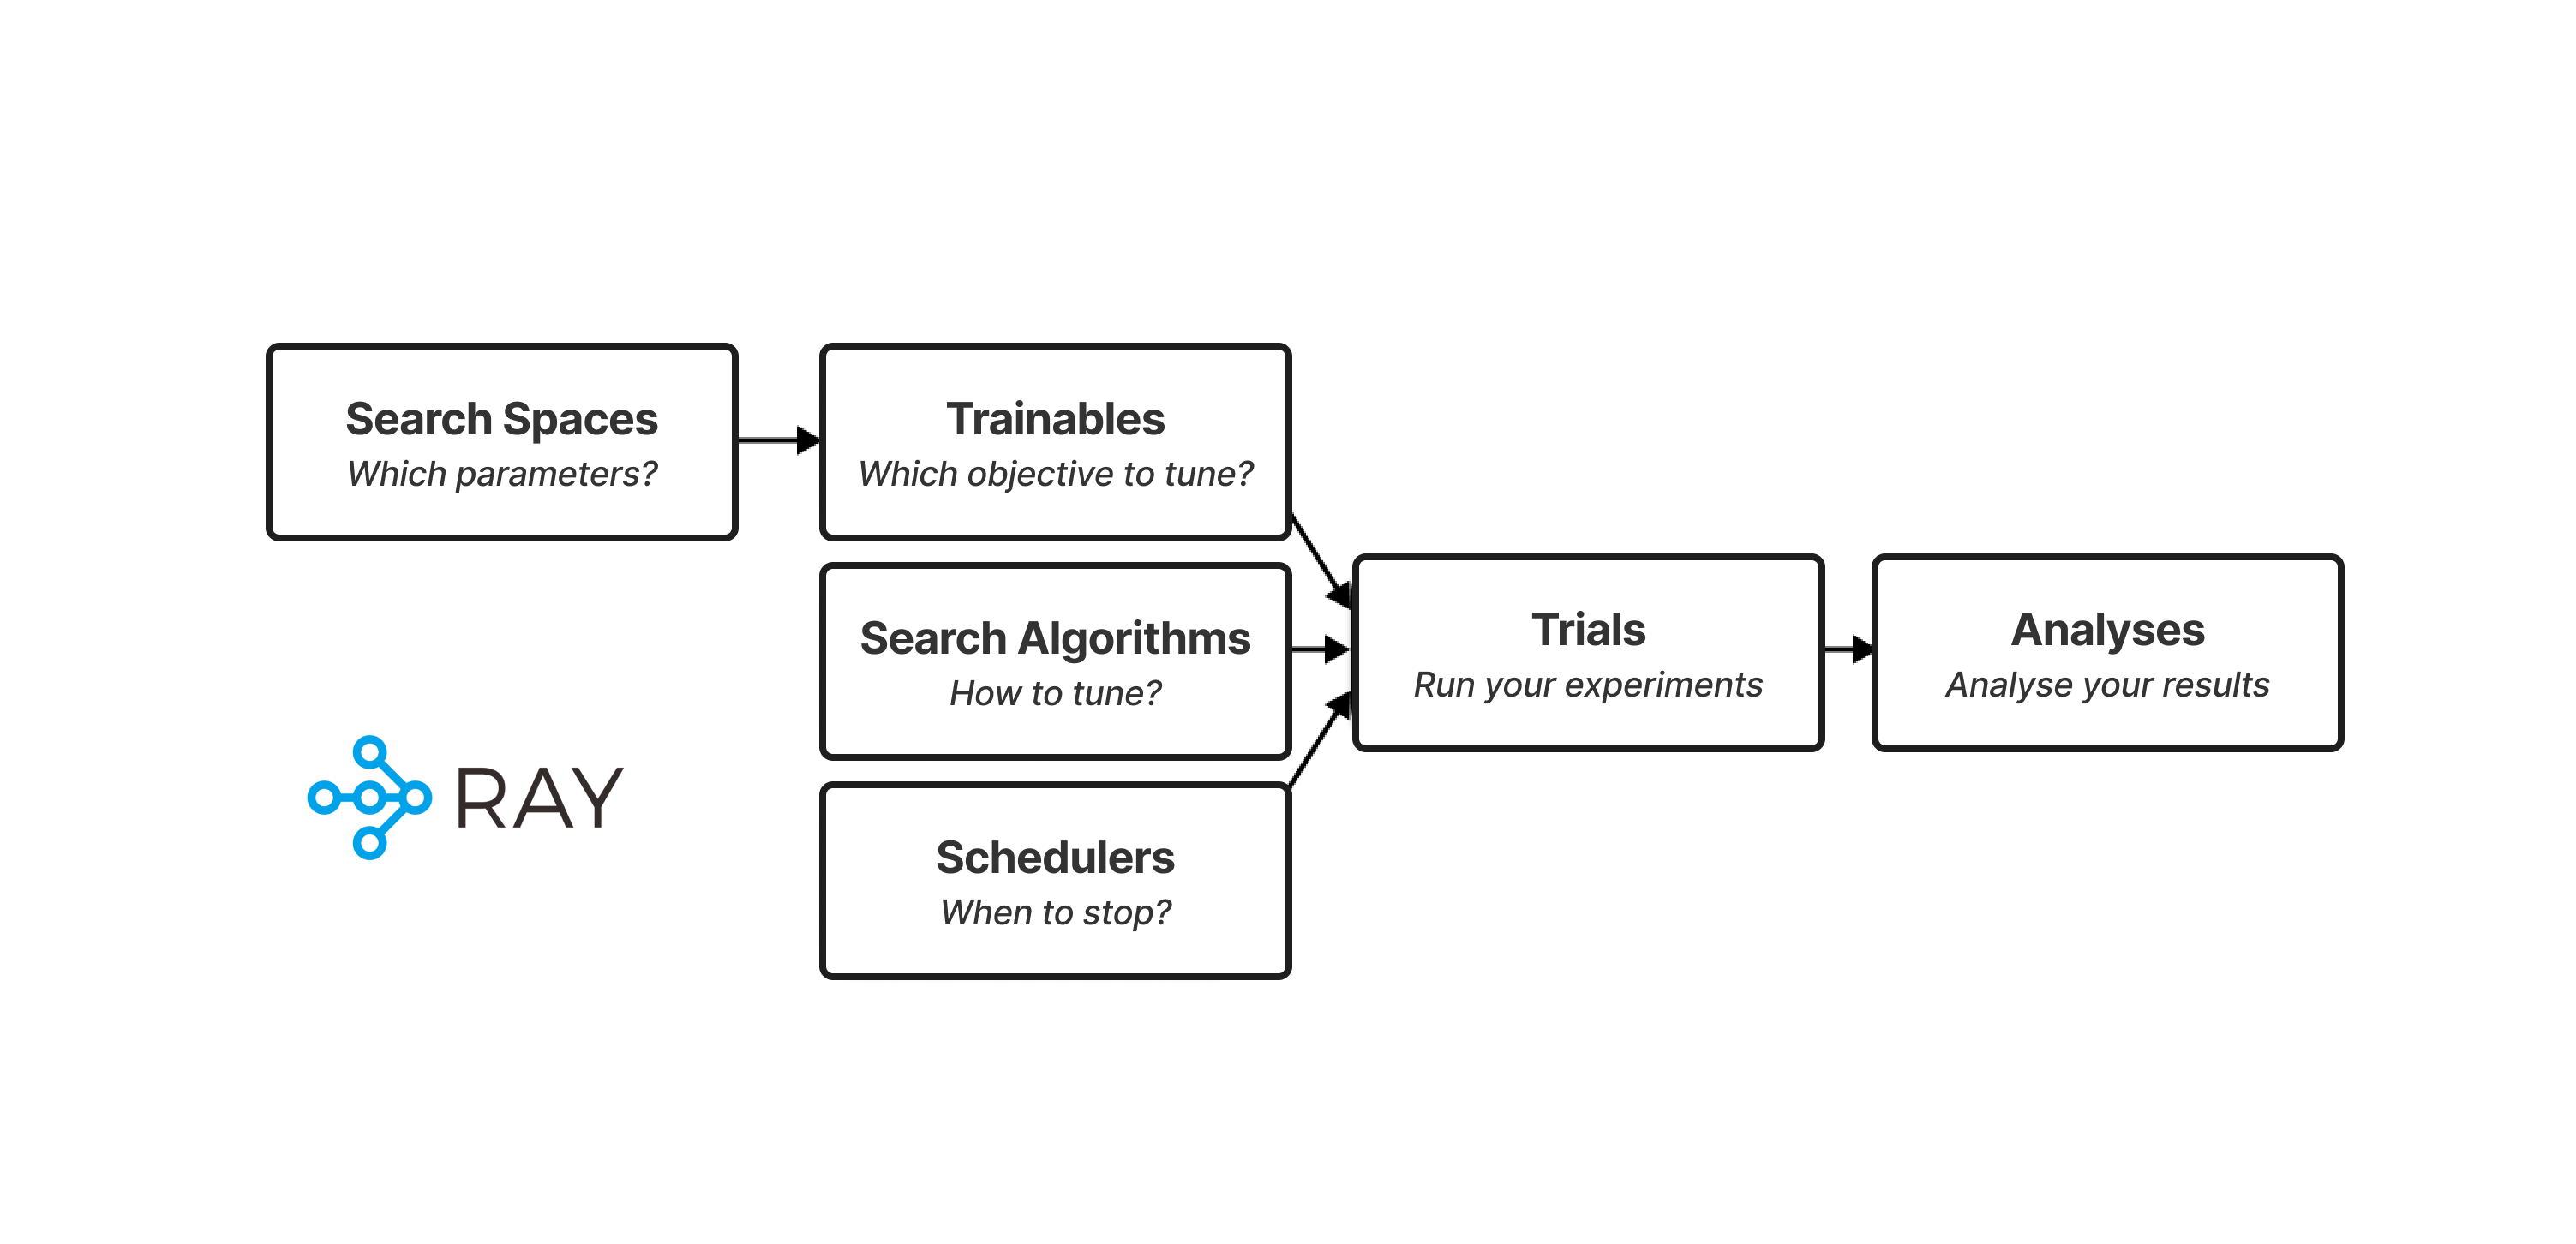
\includegraphics[width=0.9\textwidth]{Figures/Chapter 4/Ray_Flowchart.png}
    \caption{Ray Tune process flowchart}
    \label{fig:rayprocessflowchart}
\end{figure}

\subsubsection{irace}
irace (Iterated Racing) is a powerful tool designed for the automatic configuration and optimization of hyperparameters, widely used in optimization and machine learning problems. irace makes use of iterated racing algorithms to find the optimal set of hyperparameters by experimenting with many of them and discarding less good ones early on in the run, thereby reducing computation power and time. irace is particularly useful when dealing with complex models that require fine-tuning, as it balances exploration and exploitation to identify the most effective configurations. Its ability to handle discrete, continuous, and categorical parameters to produce adaptive hyperparameter optimization over a broad spectrum of ML and DL tasks makes it a flexible and adaptable tool.\cite{lopez2016irace}

\subsection{Methods for HPO}
Some of the common approaches to Hyperparameter Optimization (HPO) are:

\subsubsection{Genetic Algorithms}
Genetic Algorithms (GA) is a genetic-based evolutionary optimization algorithm derived from the rules of natural selection and genetics. They operate by keeping a set of prospective solutions that over successive rounds evolve through processes like selection, crossover and mutation. GA is an optimization algorithm that uses a population to generate diverse solutions and find optimal configurations by controlling the two competing objectives—exploration and exploitation in the search space.This recurrence approach helps to discover high-performance solutions without evaluating all possible combinations, causing GA to become particularly effective when the search space is large and the relationship between variables is complex. \cite{shanthi2022genetic}

\begin{figure}[H]
\centering
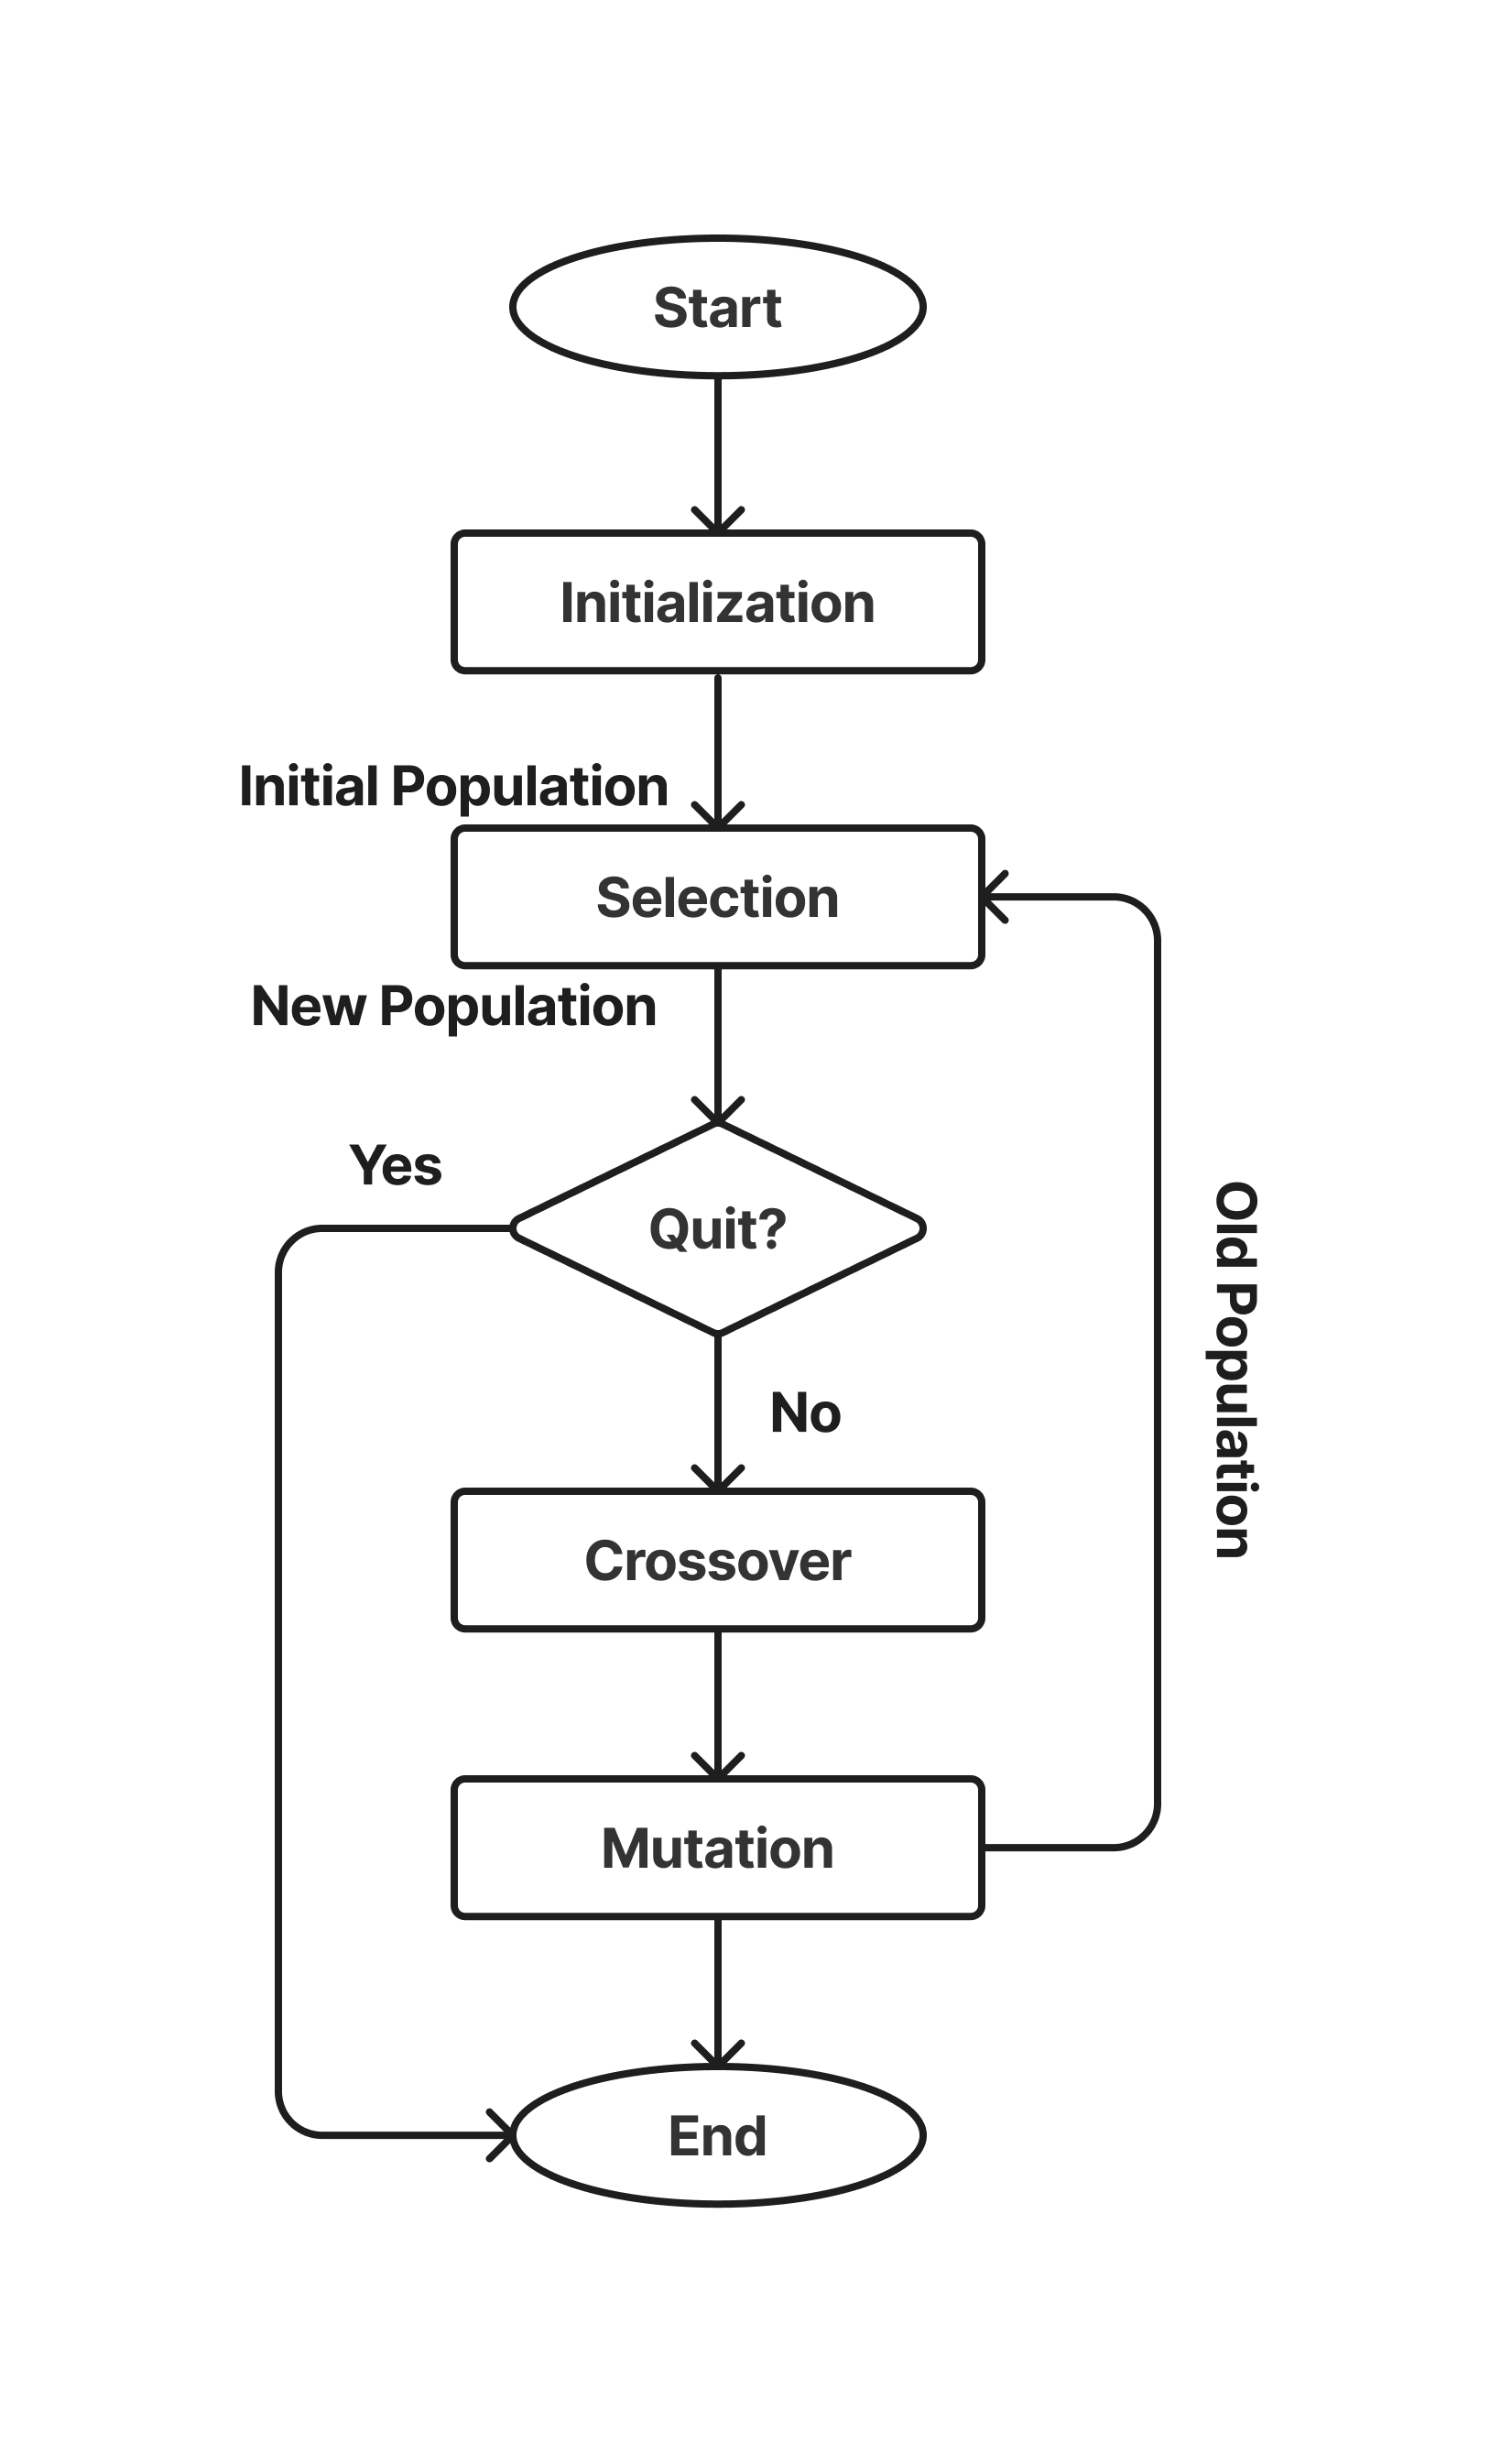
\includegraphics[width=0.55\textwidth]{Figures/Chapter 4/GA_flowchart.png}
\caption{Genetic Algorithm Process Flowchart \cite{dataset}.}
\label{fig:ga_flowchart}
\end{figure}


\subsubsection{Particle Swarm Optimization}
PSO is a population based optimization algorithm inspired by the social behavior of birds and fish. In PSO, a swarm of solutions (called particles) traverses the search space, where each particle updates its position based on its own experience and the experience of adjacent particles. By balancing exploration of new locations and exploitation of already known good solutions, each particle would update its velocity and position. The top-down, cooperative mechanism makes PSO much more likely to lead the population to optimal solutions, especially for problems with large and complex search spaces. \cite{indrawati2023enhancing}


\section{HPO: Optimized OCR models for Medical Labels using \textbf{Optuna}}
%...
This section focuses on the use of Optuna for hyperparameter optimization (HPO) applied to OCR models designed for medical label recognition. The goal is to improve model performance by systematically tuning key parameters such as learning rate, batch size, optimizer type, and others. Optuna's efficient sampling methods allow for a more guided and informed search through the hyperparameter space. The following subsection outlines the main steps involved in the optimization process using Optuna.

\subsection{Principle steps for HPO with Optuna}
%here you put a short description then you include the flow chart
Optuna performs hyperparameter optimization through a structured yet flexible process that efficiently explores the search space. As shown in Figure~\ref{fig:optuna_flowchart}, the workflow begins with the definition of the objective function and the search space, where the user specifies which hyperparameters to tune and their respective ranges or distributions.

Optuna then iteratively launches trials, each corresponding to a unique combination of sampled hyperparameters. For every trial, a model is trained using the selected parameters and then evaluated on a validation or test set using the defined objective metric. The results of each trial are stored in a database for tracking and analysis.

Throughout the process, Optuna employs advanced techniques like Tree-structured Parzen Estimator (TPE) sampling and pruning strategies to stop unpromising trials early, which helps reduce computation time. After completing all trials, Optuna selects the model configuration that achieved the best performance, which is then considered the optimal set of hyperparameters.

\begin{figure}[H]
\centering
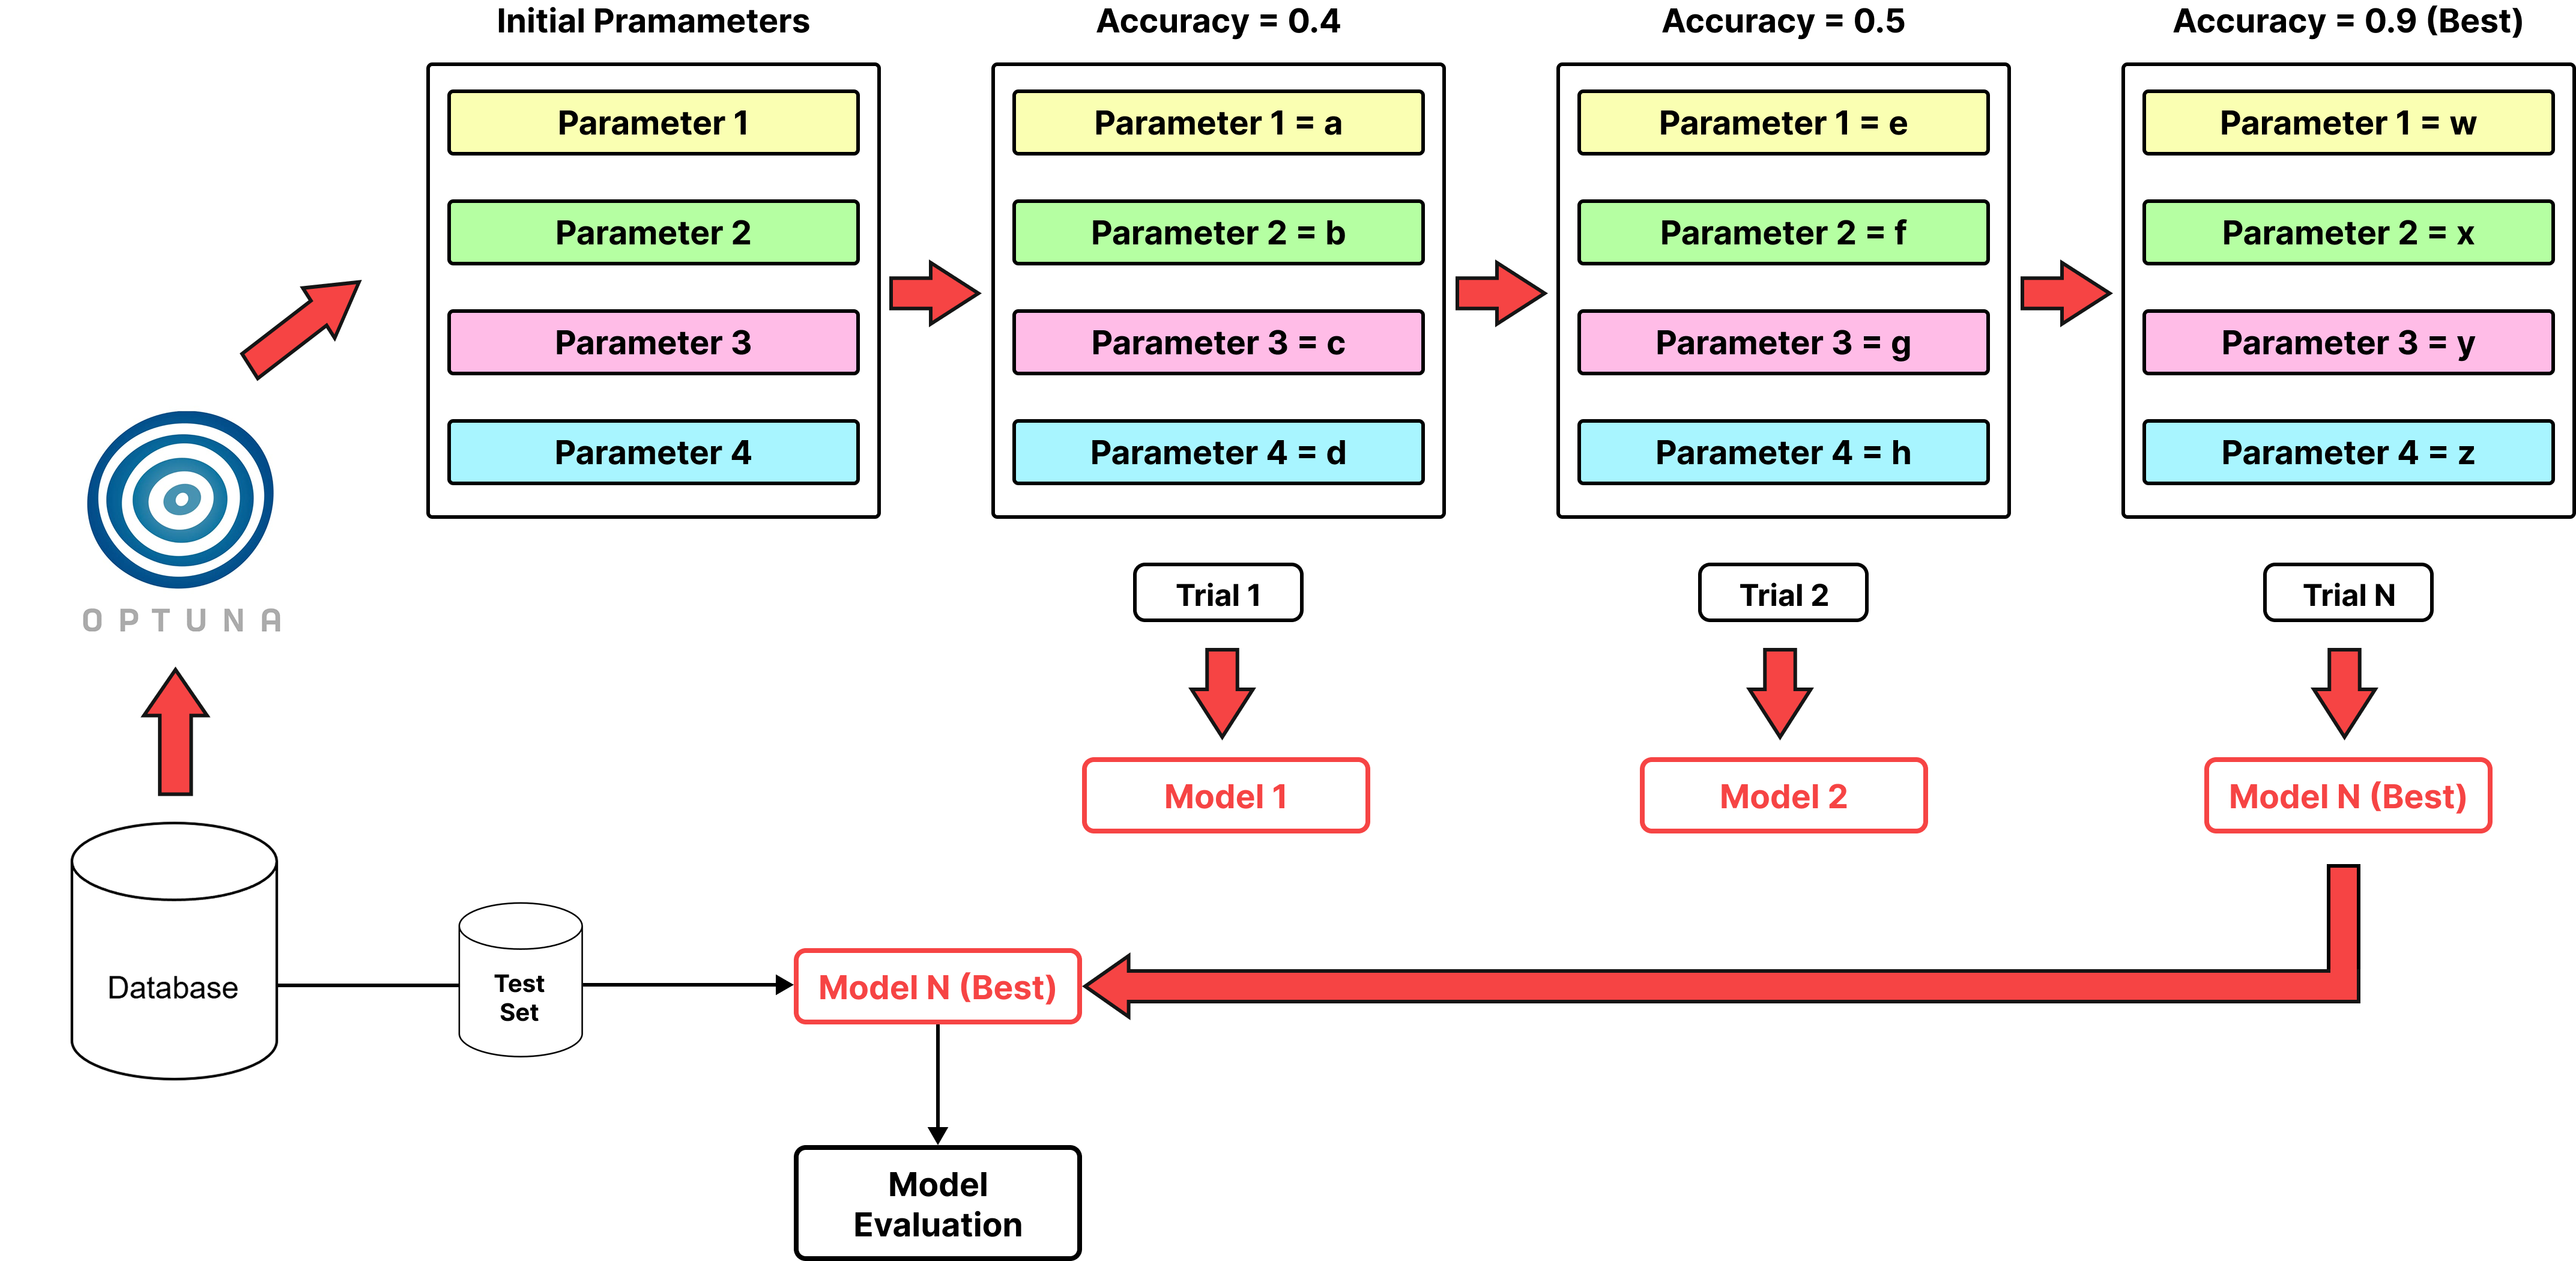
\includegraphics[width=\textwidth]{Figures/Chapter 4/Optuna_Optimization_Process.png}
\caption{Principle Steps of HPO with Optuna.}
\label{fig:optuna_flowchart}
\end{figure}

\subsection{Tesseract Hyperparameter Optimization: Description and Experimental Results}

To further improve model's performance, we used Optuna configurator to optimize Tesseract's hyperparameter values. The optimization is performed within the parameter boundaries defined in Table~\ref{tab:tesseract_hyperparameters}. The goal of Optuna is to minimize CER value on the validation set, selecting parameter value configurations that yield better generalization across varied input image qualities and text styles.

\subsubsection{Hyperparameters and Search Space}

The following table summarizes the hyperparameters optimized on Tesseract OCR model during the experiments, along with their respective ranges and descriptions:

\begin{table}[H]
\centering
\caption{Tuned hyperparameters and their search space for Tesseract HPO}
\resizebox{\textwidth}{!}{
\begin{tabular}{ccp{9.5cm}}
\hline
\textbf{Hyperparameter} & \textbf{Range/Choices} & \textbf{Description} \\
\hline
\texttt{max\_iterations} & $[500, 1500]$ & Specifies the maximum number of training iterations during fine-tuning. A higher number allows for more learning steps, potentially improving convergence, but at the cost of longer training time. \\
\hline
\texttt{learning\_rate} & $[10^{-5}, 10^{-1}]$ (log scale) & Controls how much the model’s parameters are updated during each iteration. Lower values lead to more stable training, while higher values speed up convergence but may overshoot optimal solutions. \cite{Goodfellow-et-al-2016} \\
\hline
\texttt{momentum} & $[0.1, 0.9]$ & Momentum helps accelerate the optimizer in the relevant direction by adding a fraction of the previous update to the current one, improving convergence speed and reducing oscillation. \cite{sutskever2013importance} \\
\hline
\texttt{adam\_beta} & $[0.9, 0.999]$ & The $\beta_2$ parameter of the Adam optimizer, which controls the exponential decay rate for the second moment estimates (squared gradients). Higher values retain longer-term gradient information. \cite{kingma2014adam} \\
\hline
\texttt{weight\_range} & $[0.1, 0.5]$ & Sets the initial weight range for the network during training. Affects how the model starts learning. Karger ranges can introduce more variation, while smaller ranges keep the initialization closer to zero. \\
\hline
\end{tabular}}
\label{tab:tesseract_hyperparameters}
\end{table}

%\subsubsection*{Experimental Setup}

%The hyperparameter optimization for Tesseract OCR is done first using Optuna. The process involved running the Tesseract training executable (\texttt{lstmtraining.exe}) through Python’s subprocess module, allowing Optuna to test different hyperparameter combinations automatically.

%For each trial, the script would launch a training session with the suggested hyperparameters and save the training logs. These logs were then parsed to extract the Best Character Error Rate (BCER) and the checkpoint of the best model from that trial.

%To speed up training, each new trial started from the best checkpoint found in the previous trial whenever possible; if not, it used the initial model checkpoint.

%The optimization is carried out with 30, 50, and 100 trials to see how the number of trials affected the tuning process and results.

\subsubsection{Results Summary}

To evaluate the impact of the number of trials on the performance of the Tesseract OCR model, we conducted three separate Optuna optimization studies with 30, 50, and 100 trials respectively. The results below summarize the best and average performance metrics, as well as the corresponding hyperparameter configurations.

\begin{table}[!htbp]
\centering
\caption{Best Trials results in Tesseract Optuna HPO}
\resizebox{\textwidth}{!}{
\begin{tabular}{llllr}
\hline
\textbf{Trials} & \textbf{Training Acc(\%)} & \textbf{Validation Acc(\%)} & \textbf{CER} & \textbf{Avg CER} \\
\hline
30 Trials & \textbf{77.99 (Trial 9)} & 65.70 (Trial 8) & \textbf{0.133 (Trial 15)}& \textbf{0.216 }\\
50 Trials & 77.57 (Trial 11) & \textbf{65.93 (Trial 19)} & 0.132 (Trial 26)& 0.225 \\
100 Trials & 77.94 (Trial 29) & 65.90 (Trial 93) & 0.131 (Trial 31)& 0.223 \\
\hline
\end{tabular}}
\label{tab:tesseract_optuna_best_metrics}
\end{table}

\begin{comment}
\begin{table}[htbp]
\centering
\caption{Average values of Tesseract metrics across the Trials}
\begin{tabular}{lccc}
\hline
\textbf{Trials} & \textbf{Avg Train Accuracy} & \textbf{Avg Val Accuracy} & \textbf{Avg CER} \\
\hline
30 Trials & 72.72 & 63.32 & \textbf{0.216} \\
50 Trials & 72.49 & 63.18 & 0.225 \\
100 Trials & \textbf{ 72.79} & \textbf{63.48} & 0.223 \\
\hline
\end{tabular}
\label{tab:tesseract_ocr_average_metrics}
\end{table}
\end{comment}


\begin{table}[!htbp]
\centering
\caption{Best Tesseract hyperparameters and corresponding CER}
\begin{tabular}{lccccc}
\hline
\textbf{Trials} & \texttt{learning\_rate} & \texttt{momentum} & \texttt{adam\_beta} & \texttt{weight\_range} & \textbf{CER} \\
\hline
30 Trials & 5.62e-02 & 0.3360 & 0.9942 & 0.2960 & 0.1330 \\
50 Trials & 5.59e-03 & 0.2910 & 0.9180 & 0.1310 & 0.1320 \\
100 Trials & 4.15e-03 & 0.7360 & 0.9296 & 0.4990 & \textbf{0.1310} \\
\hline
\end{tabular}

\label{tab:tesseract_optuna_best_hyperparameters}
\end{table}

Table~\ref{tab:tesseract_optuna_best_metrics} presents the best observed values for training accuracy, validation accuracy, and character error rate (CER) obtained from the Tesseract OCR model after hyperparameter optimization using Optuna. The table highlights the specific trials that yielded these optimal results. Notably, the lowest CER value of 0.131 is achieved with 100 trials, while the highest training accuracy of 77.99\% is obtained with 30 trials.

%Table~\ref{tab:tesseract_ocr_average_metrics} summarizes the average performance metrics across all trials within each optimization study. These averages provide insights into the overall optimization stability and consistency. Although 30 trials achieved the lowest average CER (0.216), the 100-trial setup slightly outperformed the others in terms of average training and validation accuracy, indicating improved generalization.

%Table~\ref{tab:tesseract_optuna_best_hyperparameters} lists the hyperparameter configurations corresponding to the best CER achieved in each trial group. These include the learning rate, momentum, Adam beta, and weight range values. The results indicate that lower CERs are typically associated with smaller learning rates and moderate values of momentum and Adam beta. As the number of trials increases, Optuna is able to explore more effective hyperparameter regions, yielding better performance.

Table~\ref{tab:tesseract_optuna_best_hyperparameters} lists the hyperparameter configurations corresponding to the best CER achieved in each trial group. These include the learning rate, momentum, Adam beta, and weight range values. The results suggest that lower CERs are generally associated with smaller learning rates (e.g., $4.15 \times 10^{-3}$ at 100 trials) and moderately high values for Adam beta.

In addition, in the 30-trial study, the best configuration involved a relatively small momentum value (0.336), indicating that during early-stage searches, lower momentum values tend to yield better results. However, as the number of trials increases, slightly higher momentum values (up to 0.736 at 100 trials) appear to perform better, suggesting that the model benefits from stronger updates when enough search space has been explored. This trend reflects Optuna’s ability to adaptively refine its search toward more effective parameter regions as the number of trials increases.


\subsubsection{Visual Analysis}

    
\begin{figure}[H]
    \centering
    \begin{subfigure}[b]{0.7\textwidth}
        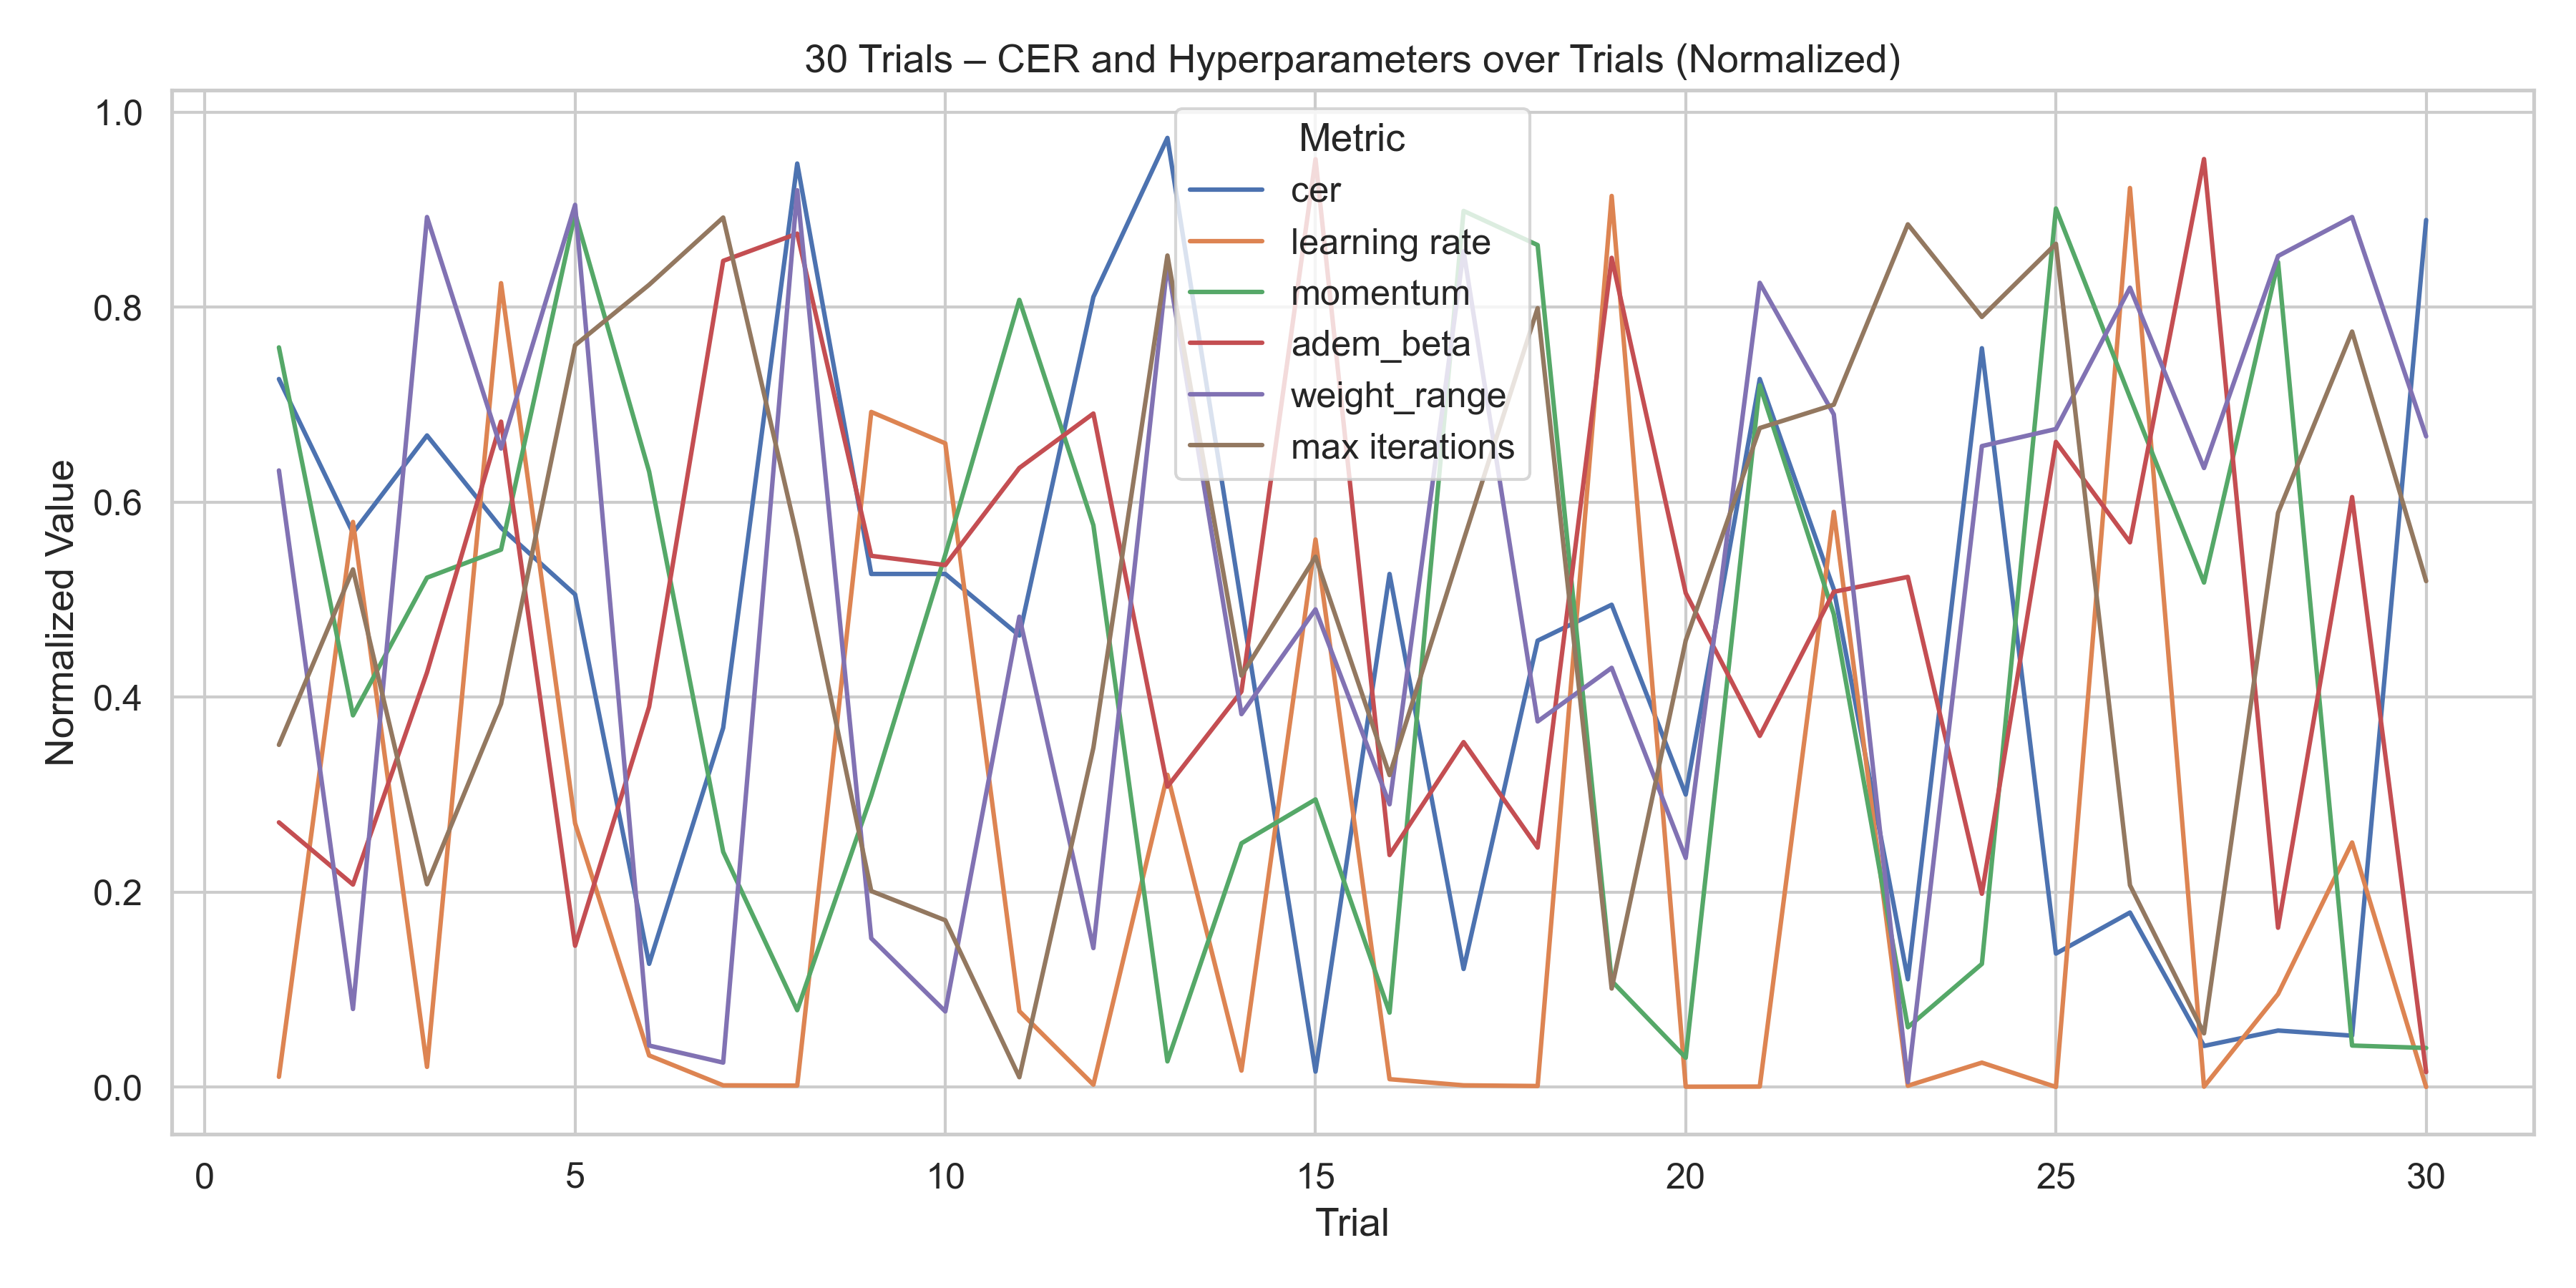
\includegraphics[width=\textwidth]{Figures/Chapter 4/tesseract_metrics_scaled_30_Trials.png}
        \caption{30 Trials}
        \label{fig:tesseract_cer_30}
       \end{subfigure}
%\end{figure}
    \vfill
%\begin{figure}
%    \centering
    \begin{subfigure}[b]{0.7\textwidth}
        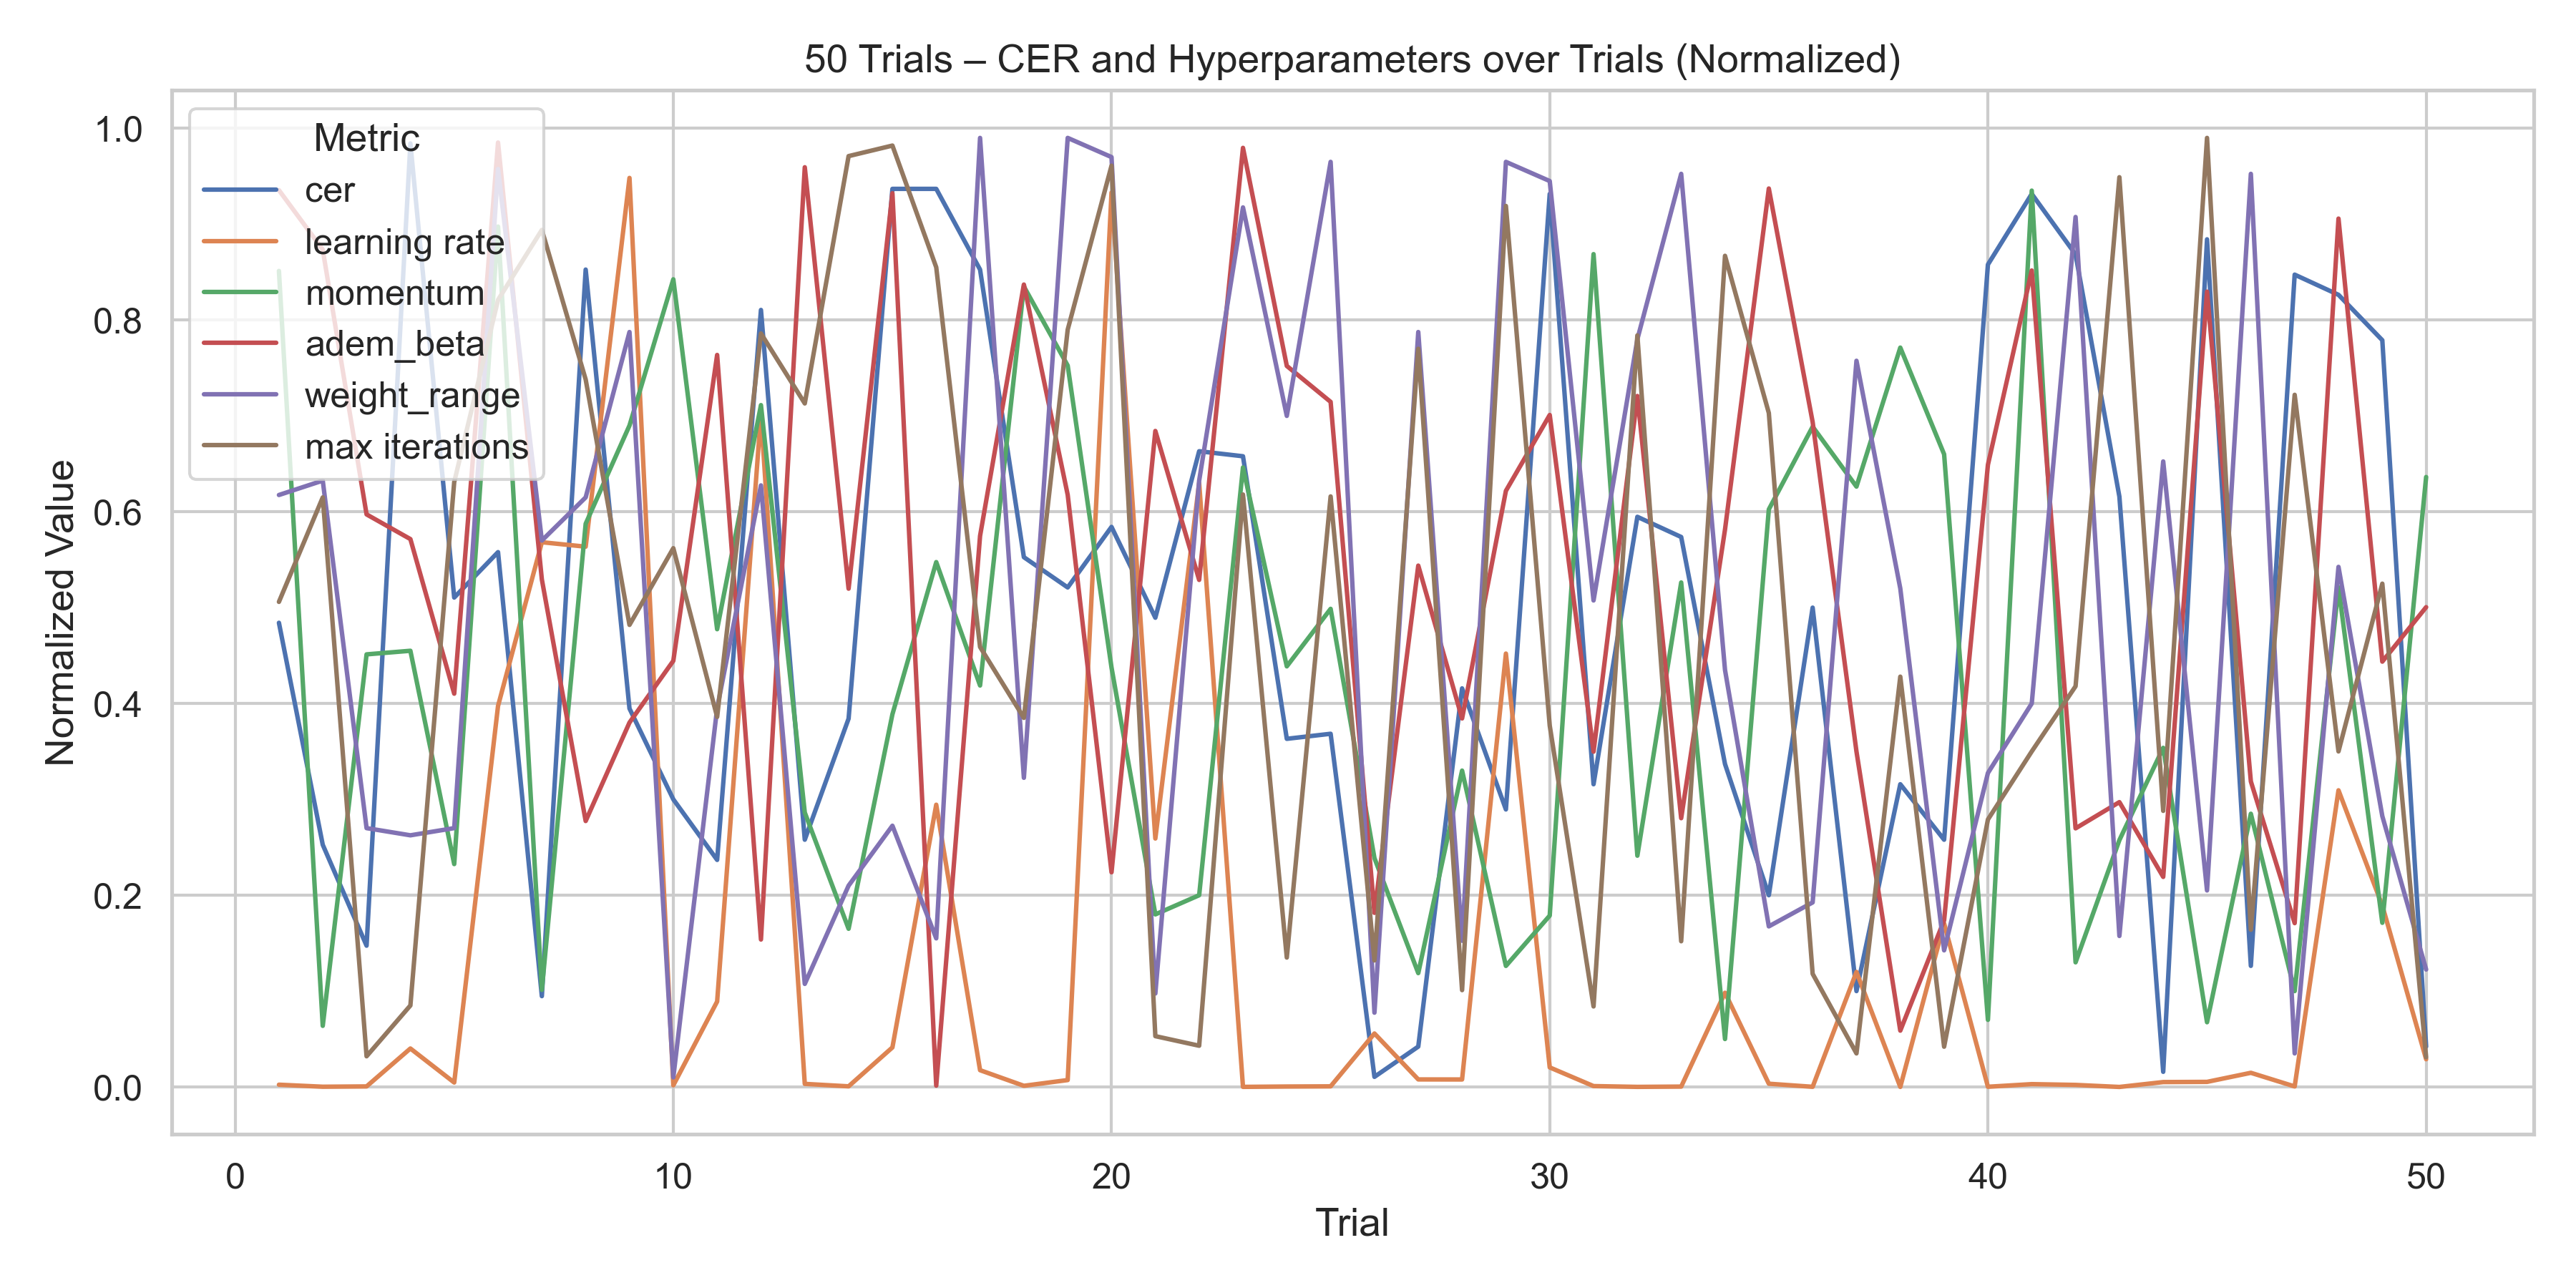
\includegraphics[width=\textwidth]{Figures/Chapter 4/tesseract_metrics_scaled_50_Trials.png}
        \caption{50 Trials}
        \label{fig:tesseract_cer_50}
    \end{subfigure}
    \vfill
    \begin{subfigure}[b]{0.7\textwidth}
        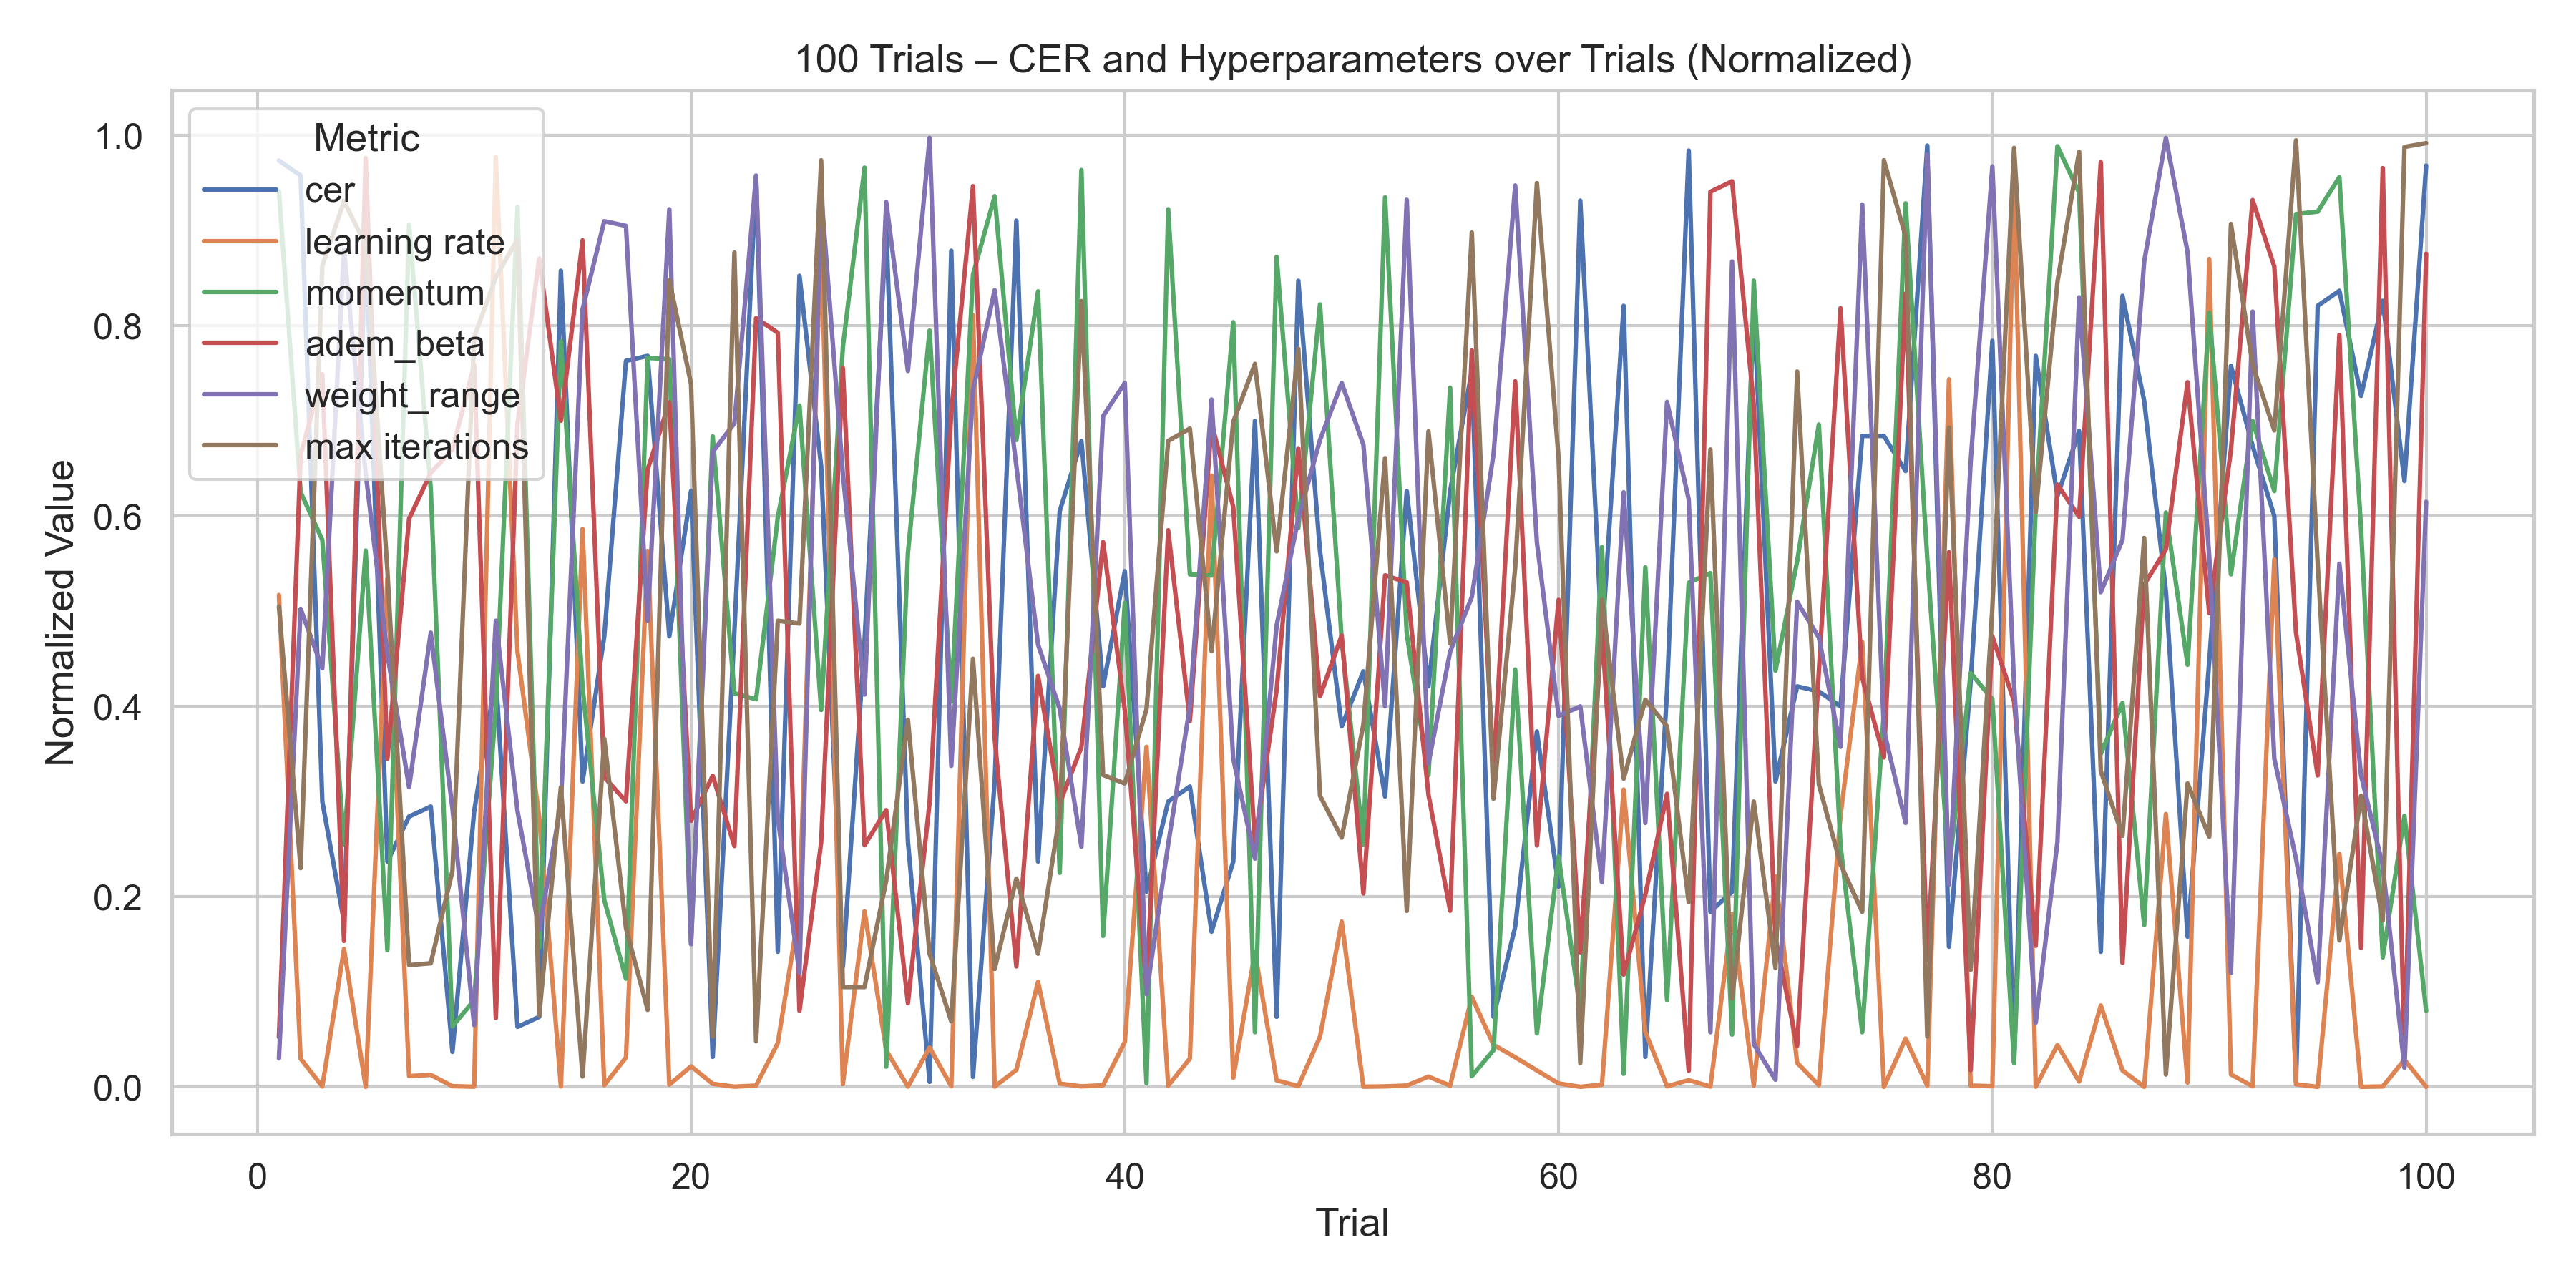
\includegraphics[width=\textwidth]{Figures/Chapter 4/tesseract_metrics_scaled_100_Trials.png}
        \caption{100 Trials}
        \label{fig:tesseract_cer_100}
    \end{subfigure}
    \caption{Evolution of CER and hyperparameter values across different trial counts in Tesseract.}
    \label{fig:tesseract_cer_all_trials}
\end{figure}

The Figure \ref{fig:tesseract_cer_all_trials} illustrates the optimization trajectory of Tesseract's CER across three different trial budgets: 30, 50, and 100. A downward trend in CER is visible, particularly with the 100-trial configuration, indicating that more trials yield better exploration and convergence. The plots also show the hyperparameter shifts during the search, such as learning rate and weight range, helping visualize how Optuna navigates the parameter space

\subsubsection{Performance Summary and Observations}
The optimization trials demonstrated clear diminishing returns, with 100 trials achieving only a marginal 0.76\% CER improvement (0.131) over 50 trials (0.132) despite doubled computational cost. Optimal configurations consistently featured moderate learning rates (10\^{-3}-10\^{-2}) and momentum values (0.2-0.4), balancing convergence speed and stability. Significant improvements occurred primarily within the first 20-30 trials, after which refinement yielded minimal gains. The persistent 12-15\% accuracy gap between training and validation performance highlights Tesseract's generalization challenges across document variations. These findings establish practical parameter ranges for efficient French OCR optimization while demonstrating the limits of extended hyperparameter search.

\clearpage
\subsection{EasyOCR  Hyperparameter optimization: Description and experimental results }

In this section, we describe the process and results of applying hyperparameter optimization to the EasyOCR text recognition model using the \textbf{Optuna} framework. The aim of this optimization is to fine-tune critical training hyperparameters to improve the performance of the model on our custom medical label dataset.

\subsubsection{Hyperparameters and Search Space}

The following table summarizes the hyperparameters optimized during the experiments, along with their respective ranges or categorical options and detailed descriptions:

\begin{table}[H]
\centering
\caption{Tuned hyperparameters and their search space for EasyOCR HPO}
\resizebox{\textwidth}{!}{
\begin{tabular}{ccp{9.2cm}}
\hline
\textbf{Hyperparameter} & \textbf{Range/Choices} & \textbf{Description} \\
\hline
\texttt{lr} & $[10^{-5}, 10^{-2}]$ (log scale) & The learning rate used by the optimizer to update model weights during training. Lower values lead to smaller weight updates and more stable convergence, while higher values can accelerate training at the risk of divergence. \cite{Goodfellow-et-al-2016} \\
\hline
\texttt{batch\_size} & \{8, 16\} & Number of training samples processed before updating model weights. Smaller batch sizes introduce more noise into updates but may generalize better, while larger batches offer smoother gradients and faster computation. \cite{masters2018revisiting} \\
\hline
\texttt{beta1} & $[0.9, 0.99]$ & The $\beta_1$ parameter in the Adam optimizer, controlling the exponential decay rate of the moving average of the gradient (first moment estimate). Influences how quickly the optimizer adapts to changes in gradient direction. \cite{kingma2014adam} \\
\hline
\texttt{rho} & $[0.95, 0.99]$ & The $\rho$ parameter in the AdaDelta optimizer, which determines the decay rate for the moving average of squared gradients. Higher values give the optimizer a longer memory. \cite{zeiler2012adadelta} \\
\hline
\texttt{eps} & $[10^{-10}, 10^{-6}]$ (log scale) & A small constant added for numerical stability to prevent division by zero during the update steps. Its value can influence convergence behavior depending on the optimizer. \cite{kingma2014adam, zeiler2012adadelta} \\
\hline
\end{tabular}}
\label{tab:easyocr_hyperparameters}
\end{table}

\subsubsection{Experimental Setup}

Hyperparameter optimization is performed using the \texttt{Optuna} framework. Each trial involved running the Tesseract training executable with a specific set of hyperparameters suggested by Optuna. The best model checkpoint from the previous trial is used to initialize training for the current trial when available.

The optimization process is carried out through three separate studies with \textbf{30}, \textbf{50}, and \textbf{100} trials respectively. The objective for Optuna is to minimize the Validation Loss, which is extracted from the training logs after each trial.


\subsubsection{Results Summary}

The following table shows the best trial results for each Optuna study in terms of recognition accuracy, Character Error Rate (CER), training loss, and validation loss:

\begin{table}[H]
\centering
\caption{Best Trials results in EasyOCR Optuna HPO}
\resizebox{\textwidth}{!}{
\begin{tabular}{lcccc}
\hline
\textbf{Trials} & \textbf{Accuracy (\%)} & \textbf{Training Loss} & \textbf{Validation Loss} & \textbf{CER} \\
\hline
30 Trials & 34.7390 (trial \#16) & 0.0899 (trial \#23) & 0.5284 (trial \#27) & 0.1160 (trial \#29) \\
50 Trials & \textbf{37.4690 (trial \#49)} & \textbf{0.0375 (trial \#49)} & 0.5241 (trial \#16) & 0.1175 (trial \#49) \\
100 Trials & 36.2280 (trial \#67) & 0.0610 (trial \#12) & \textbf{0.5052 (trial \#99)} & \textbf{0.1102 (trial \#26)} \\
\hline
\end{tabular}}
\label{tab:easyocr_optuna_best_metrics}
\end{table}


\begin{table}[H]
\centering
\caption{Average values of EasyOCR metrics across the Trials}
\begin{tabular}{lcccc}
\hline
\textbf{Trials} & \textbf{Avg Accuracy} & \textbf{Avg Train Loss} & \textbf{Avg Val Loss} & \textbf{Avg CER} \\
\hline
30 Trials & 29.6029 & \textbf{0.1712} & 0.6114 & 0.\textbf{2561} \\
50 Trials & 30.4168 & 0.1567 & \textbf{0.6196} & 0.2360 \\
100 Trials & \textbf{30.6873} & 0.1524 & 0.6069 & 0.2406 \\
\hline
\end{tabular}
\label{{tab:easyocr_optuna_average_metrics}}
\end{table}


\begin{table}[H]
\centering
\caption{Best EasyOCR hyperparameters and corresponding CER}
\begin{tabular}{lcccccc}
\hline
\textbf{Trials} & \texttt{lr} & \texttt{batch\_size} & \texttt{beta1} & \texttt{rho} & \texttt{eps} & \textbf{CER} \\
\hline
30 Trials & 4.68e-3  & 16 & 0.9237 & 0.9719 & 7.41e-10 & 0.1160 \\
50 Trials & 2.61e-4  & 16 & 0.9073 & 0.9516 & 1.65e-10 & \textbf{0.1175} \\
100 Trials & 1.08e-3  & 8  & 0.9319 & 0.9749 & 3.59e-7 & 0.1102 \\
\hline
\end{tabular}
\label{tab:easyocr_optuna_best_hyperparameters}
\end{table}

We observed that the best accuracy improved as the number of trials increased, reaching its peak at 37.4690\% in the 50-trial study. However, the lowest training loss is achieved in the same 50-trial set, while the lowest validation loss is observed in the 100-trial set, indicating some variability in where the best performance for each metric occurred. The Character Error Rate (CER) consistently decreased with more trials, with the lowest CER of \textbf{0.1102} found during the 100-trial experiment.

On average, across all trials, the metrics showed a similar trend: accuracy increased from 29.60\% (30 trials) to 30.69\% (100 trials), training loss decreased from 0.1712 to 0.1524, validation loss remained fairly stable around 0.61, and CER improved from 0.2561 to 0.2406. These average values confirm that increasing the number of trials generally improves model performance.

These results suggest that increasing the number of trials allows for better hyperparameter exploration, improving certain metrics like CER and validation loss, although the best accuracy is achieved earlier at 50 trials. The model trained with 100 trials showed the best generalization performance as indicated by the lowest validation loss and CER, reflecting a well-fit and robust model.

\subsubsection{Visual Analysis}

    \begin{figure}[H]
    \centering
    \begin{subfigure}[b]{0.7\textwidth}
        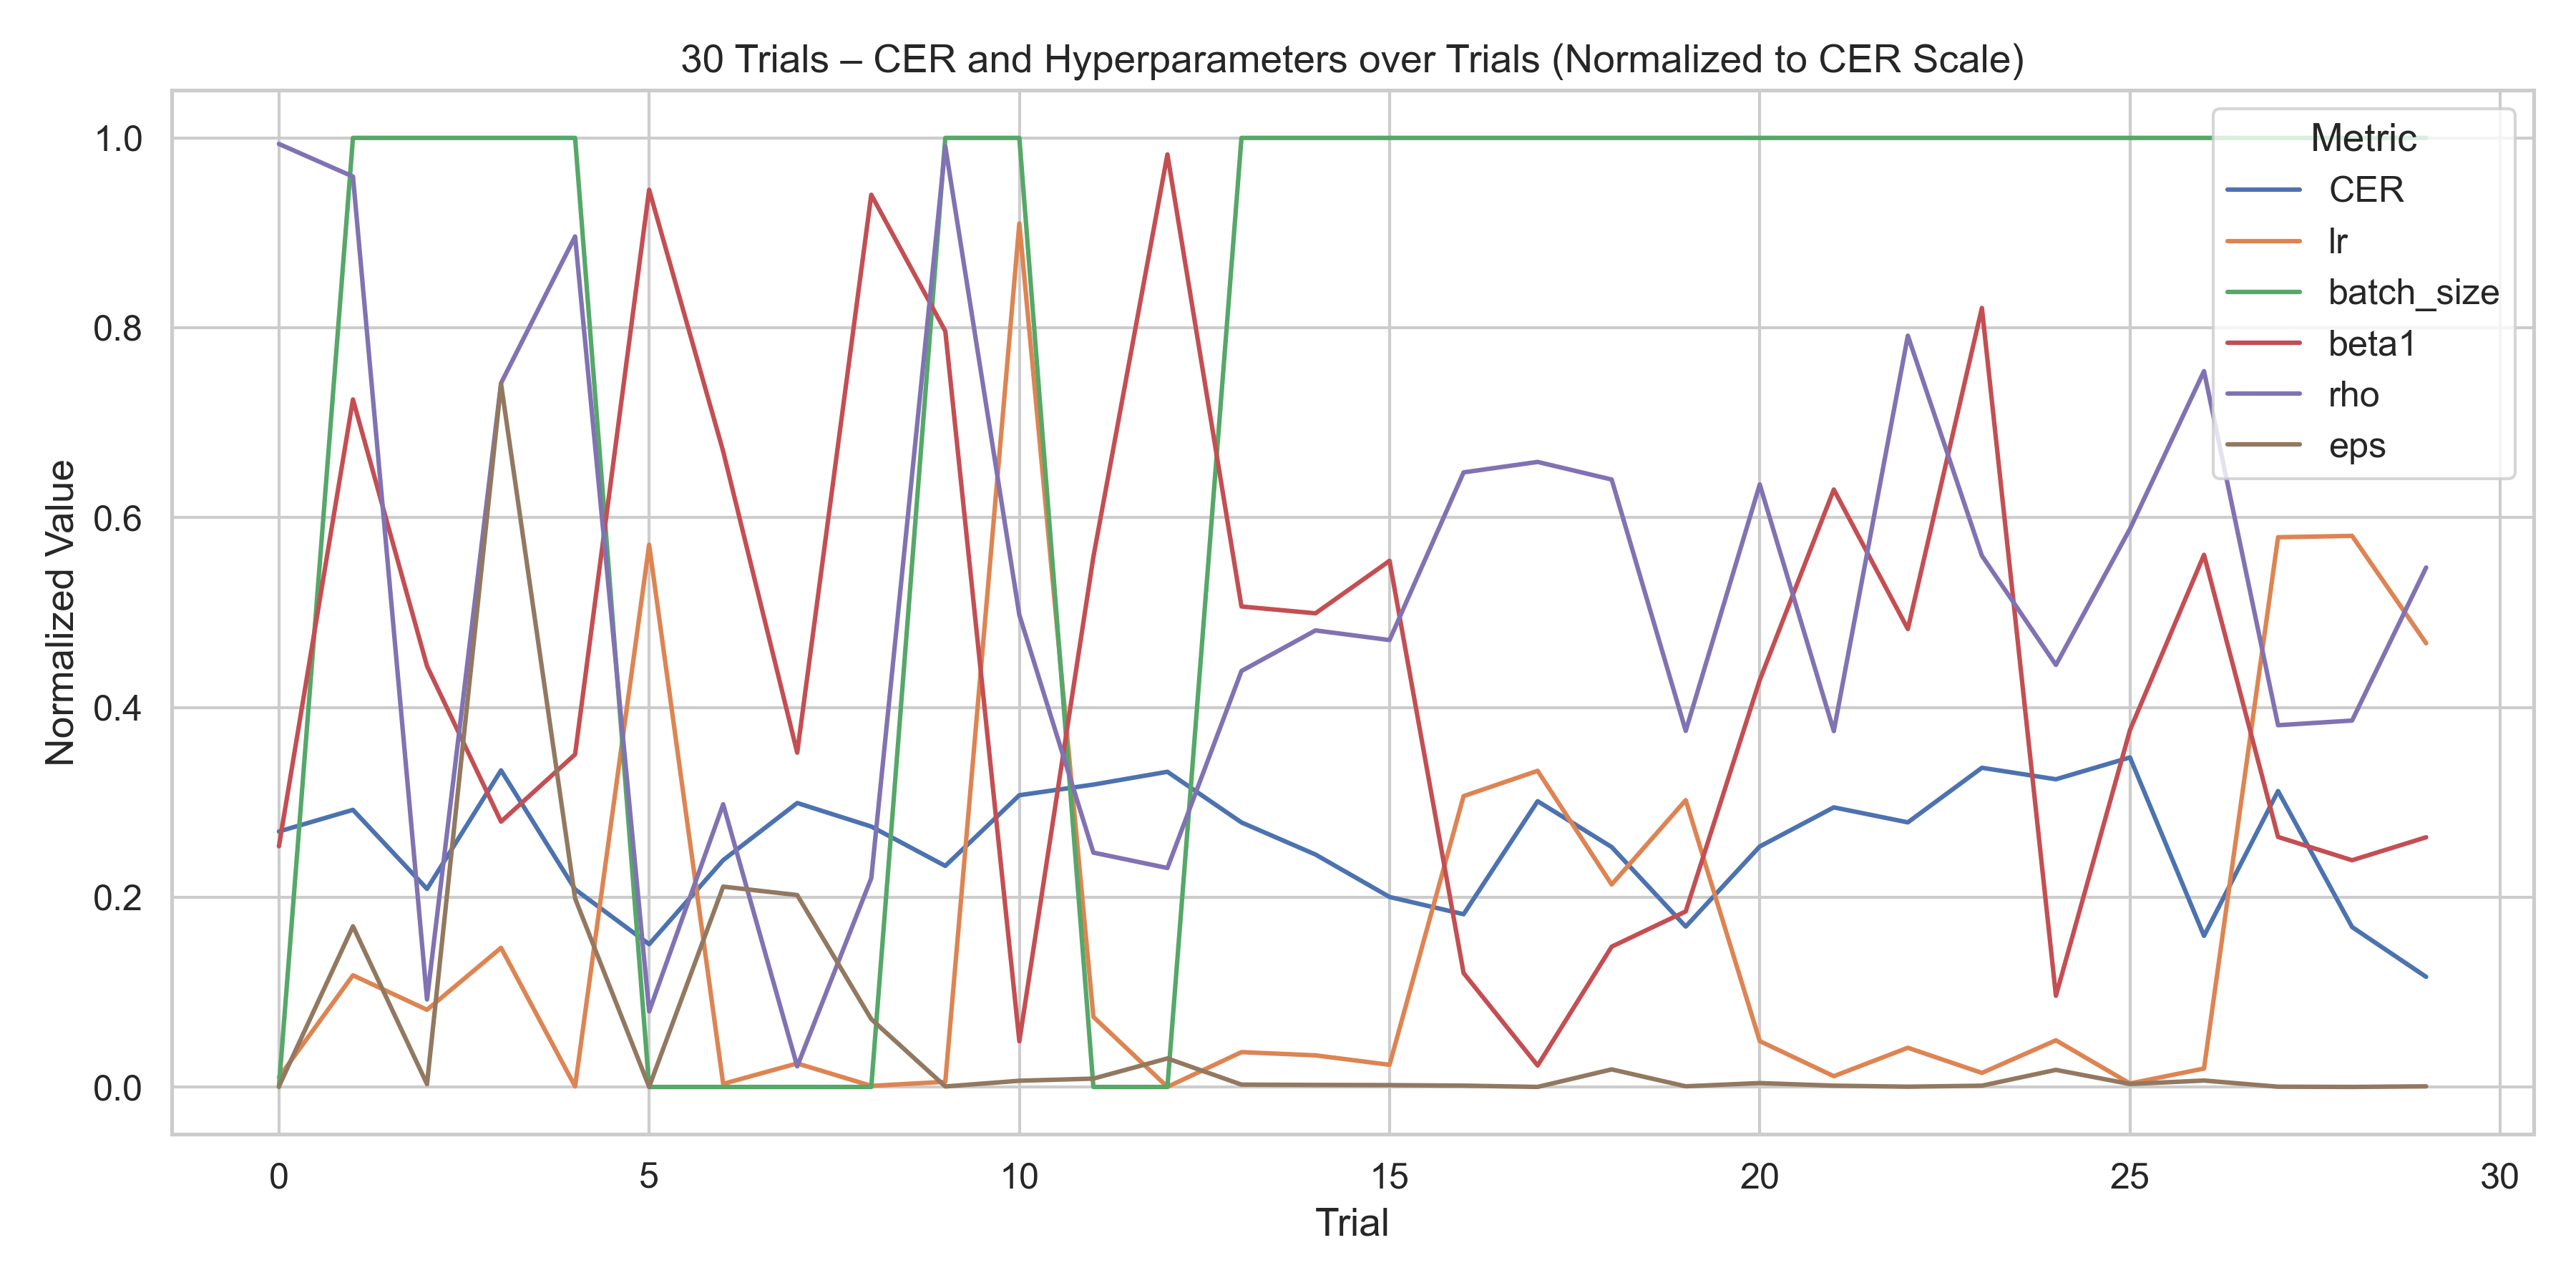
\includegraphics[width=\textwidth]{Figures/Chapter 4/trial_metrics_scaled_to_CER_30_Trials.png}
        \caption{30 Trials}
        \label{fig:cer_30}
       \end{subfigure}
%\end{figure}
    \vfill
%\begin{figure}
%    \centering
    \begin{subfigure}[b]{0.7\textwidth}
        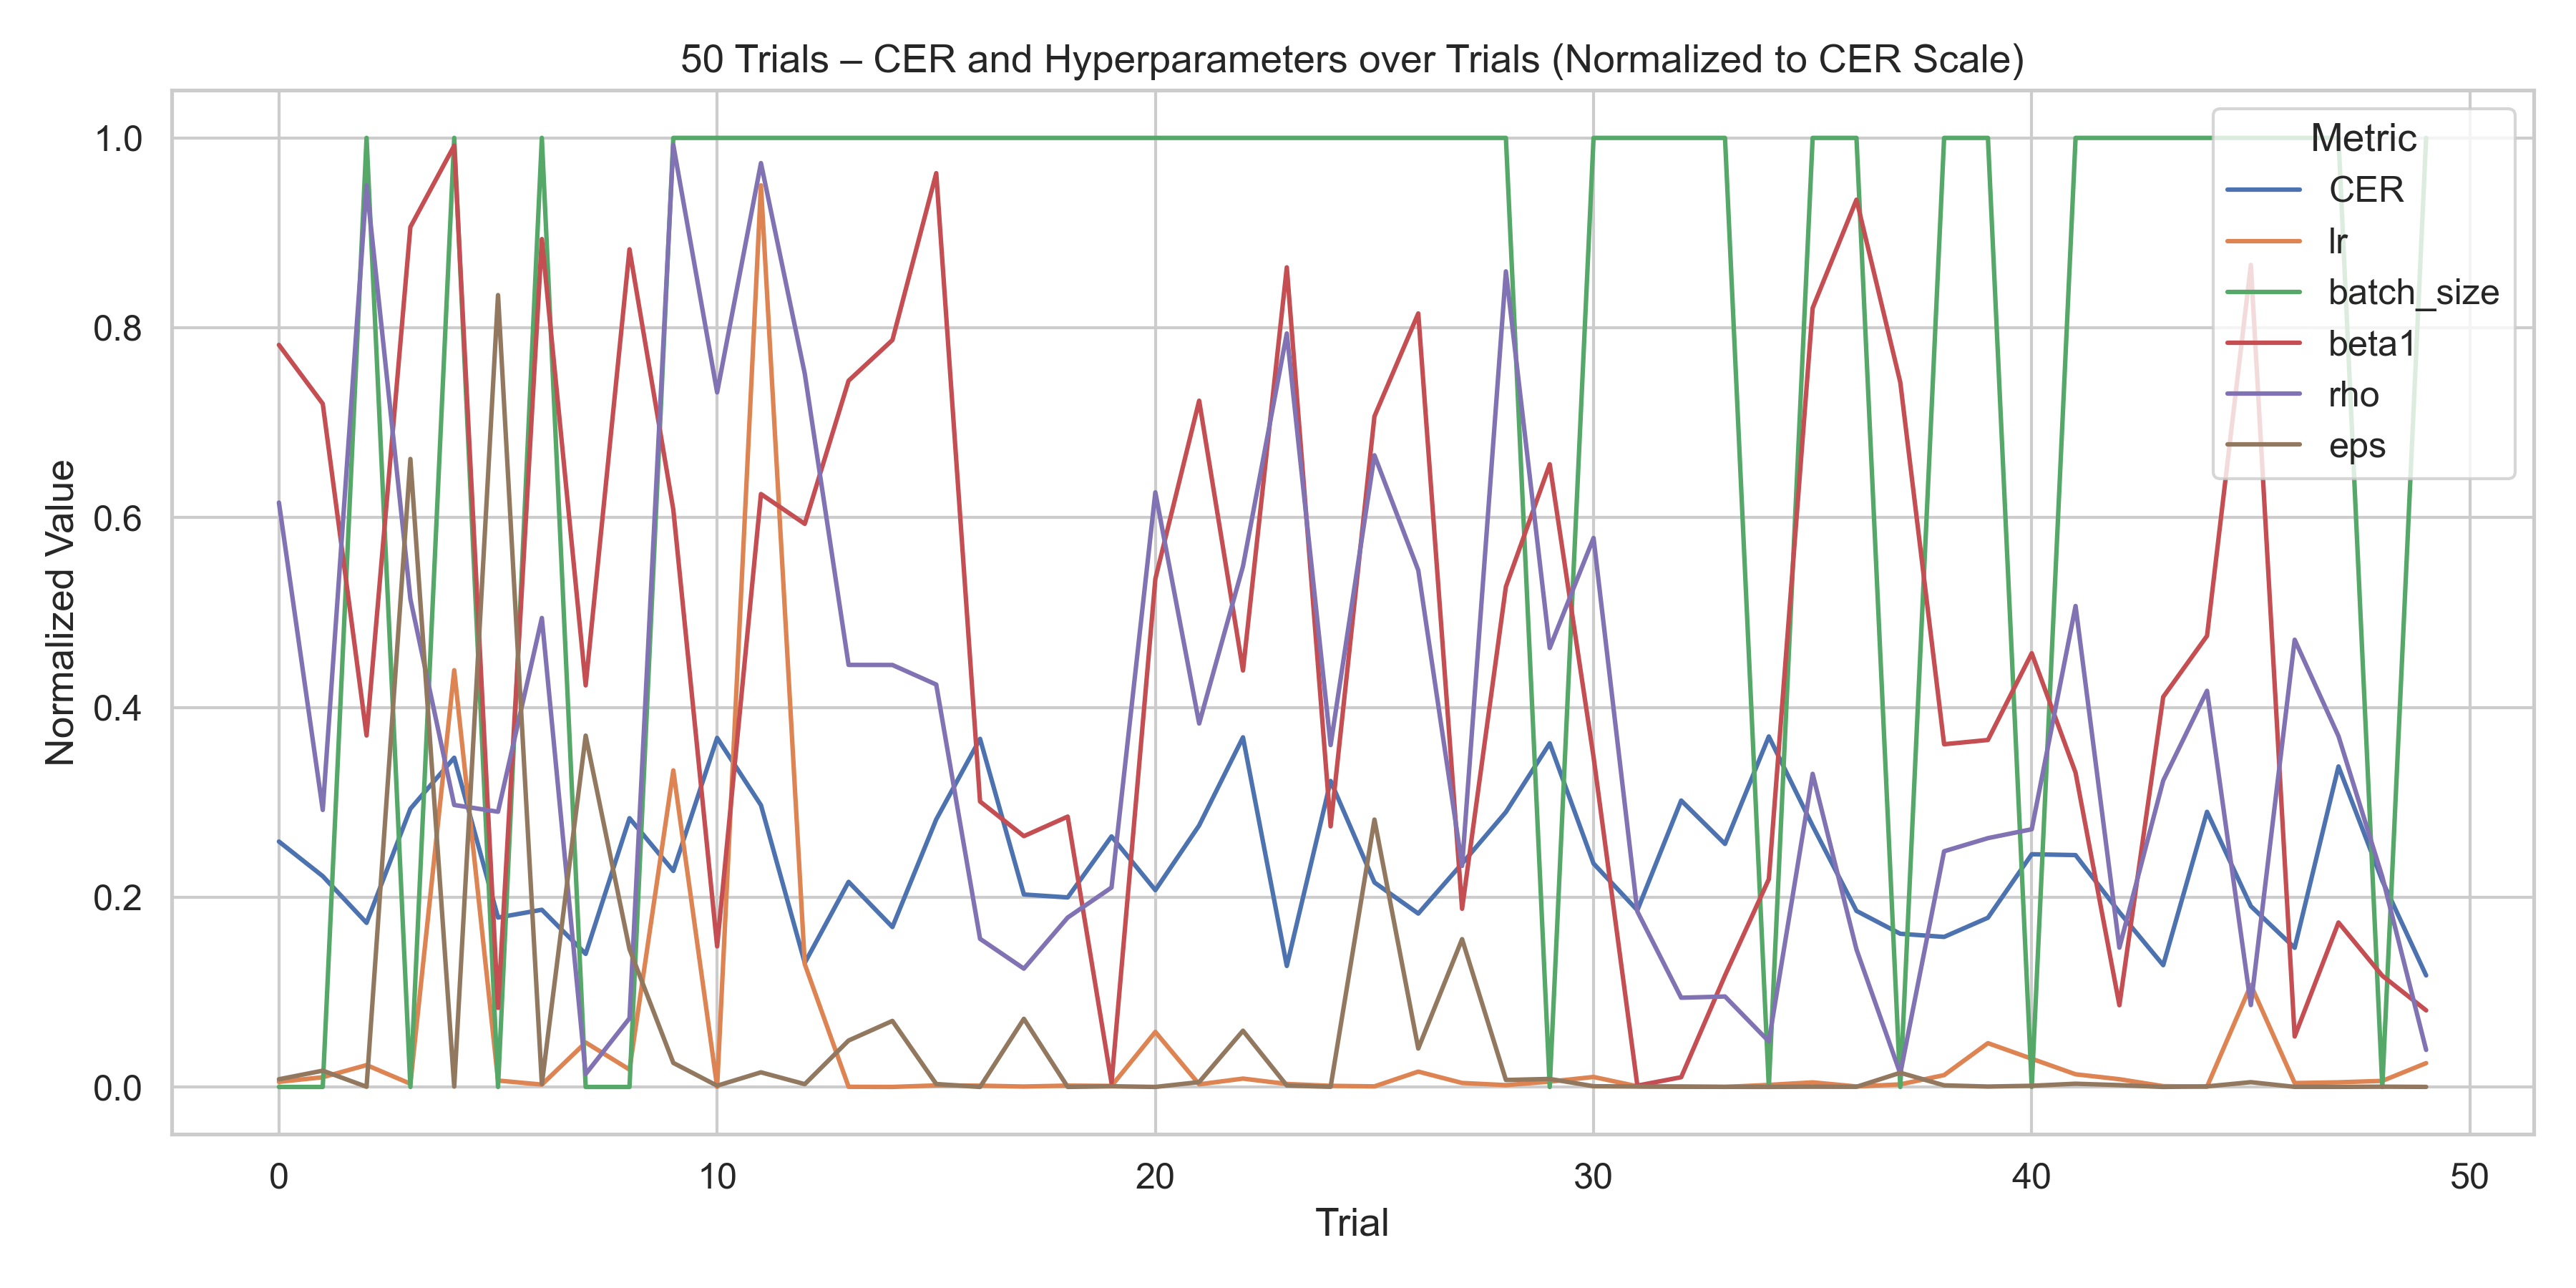
\includegraphics[width=\textwidth]{Figures/Chapter 4/trial_metrics_scaled_to_CER_50_Trials.png}
        \caption{50 Trials}
        \label{fig:cer_50}
    \end{subfigure}
    \vfill
    \begin{subfigure}[b]{0.7\textwidth}
        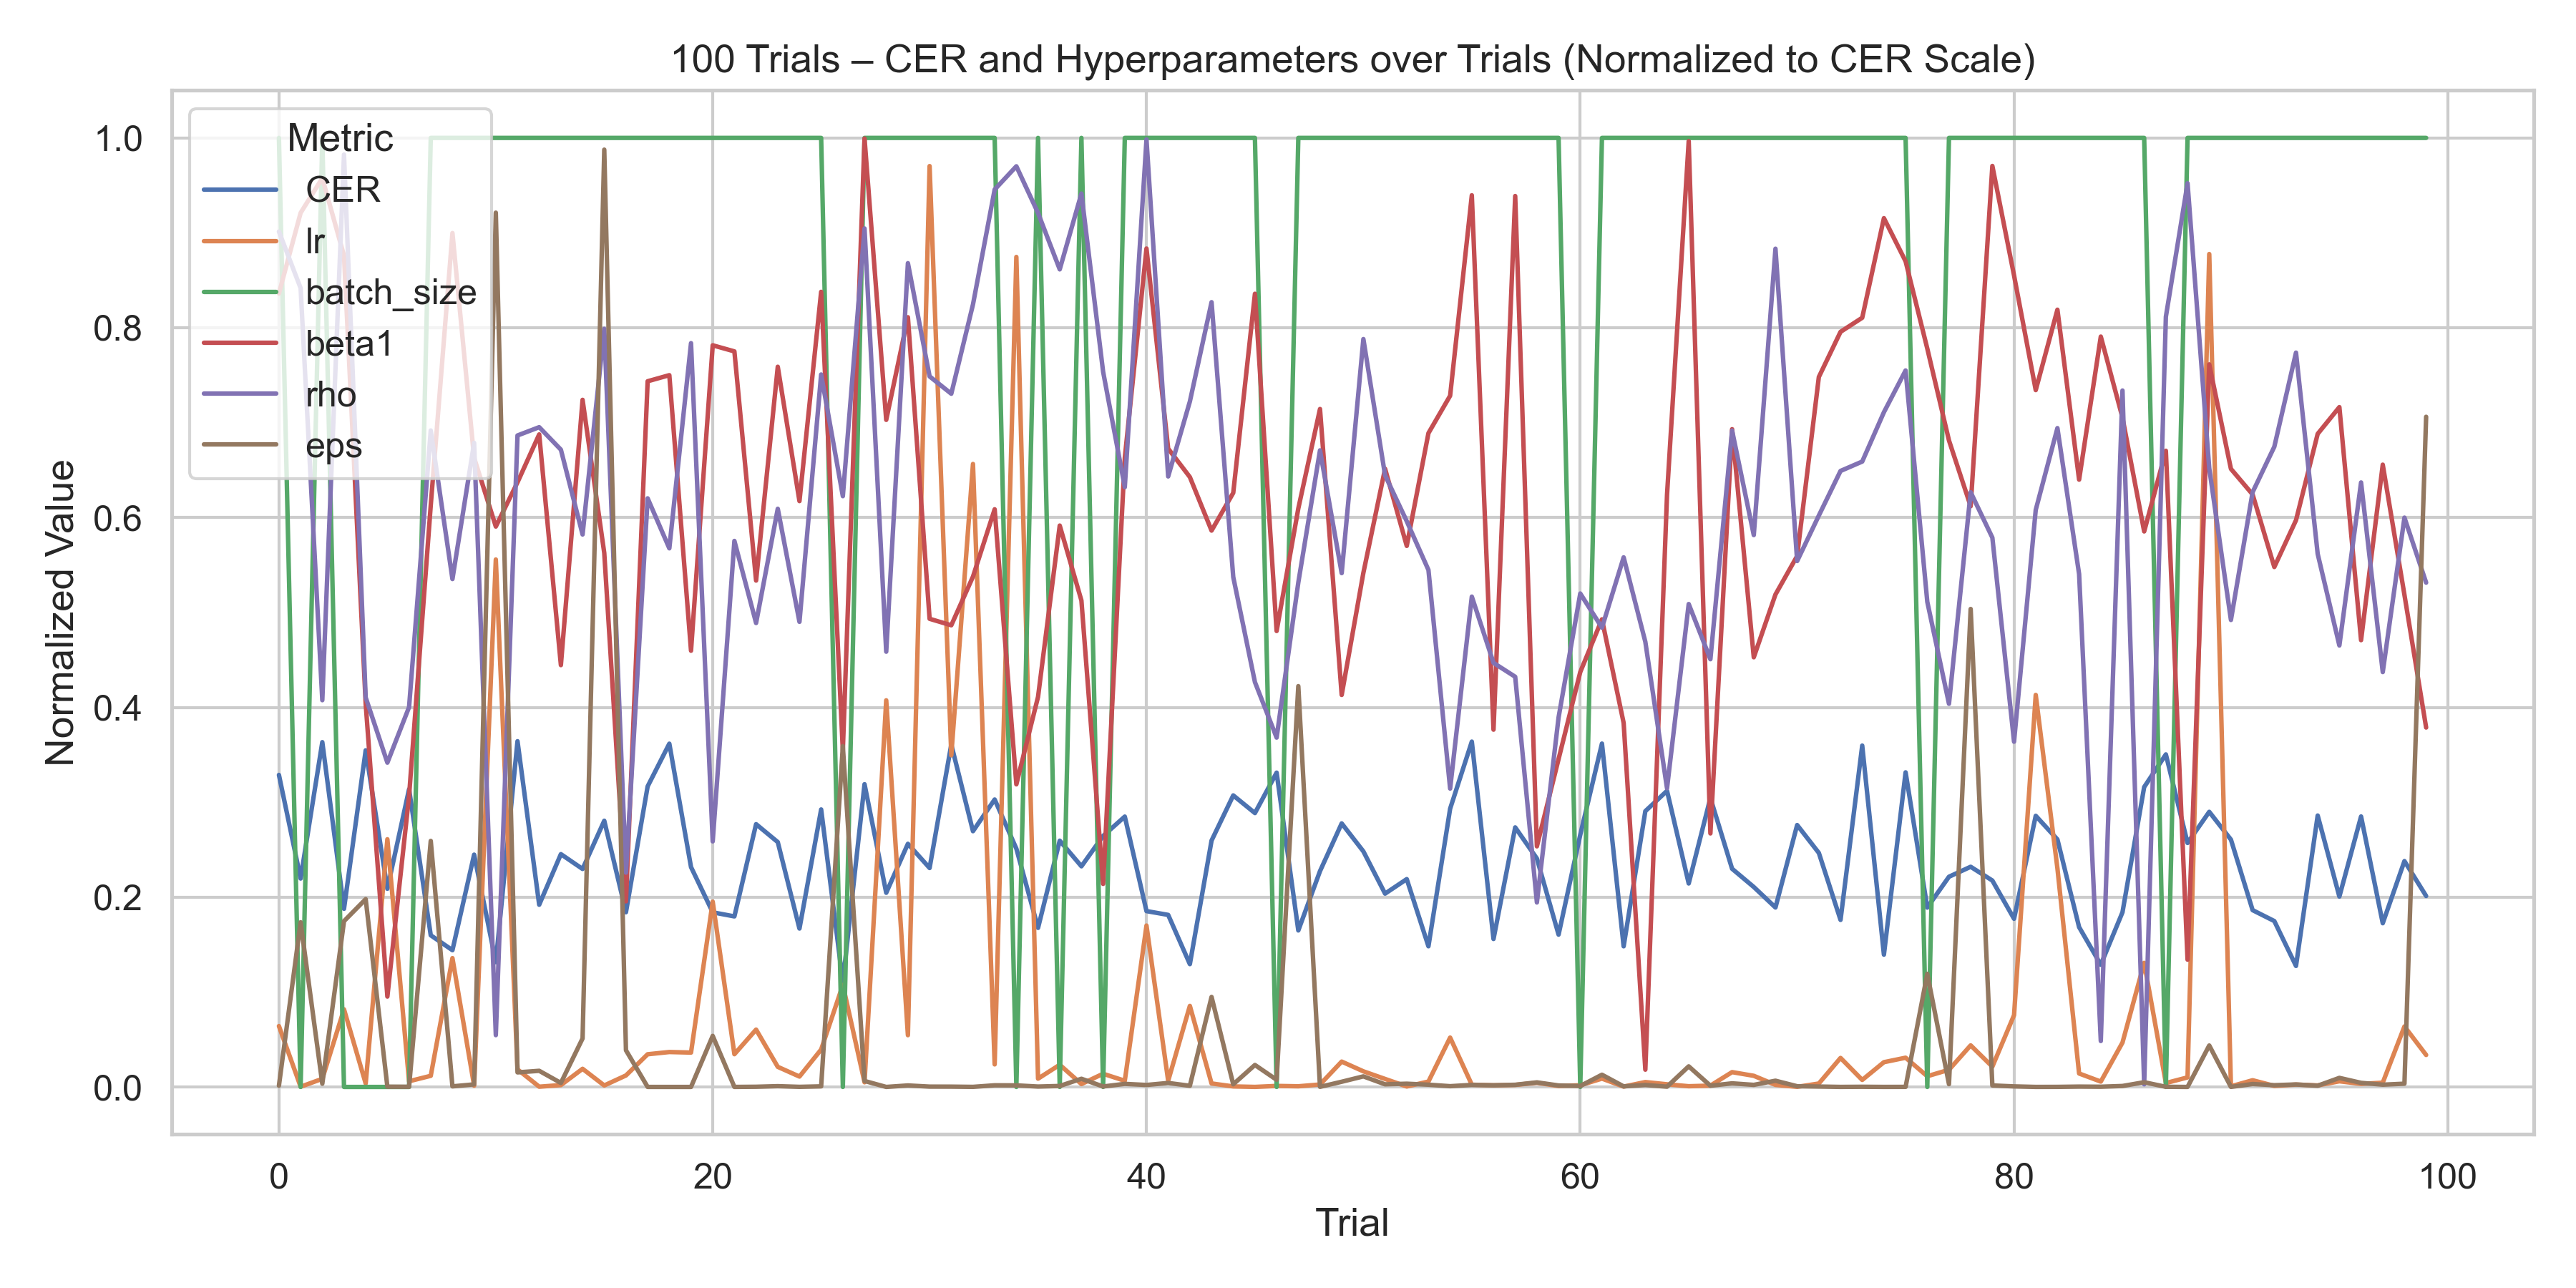
\includegraphics[width=\textwidth]{Figures/Chapter 4/trial_metrics_scaled_to_CER_100_Trials.png}
        \caption{100 Trials}
        \label{fig:cer_100}
    \end{subfigure}
    \caption{Evolution of CER and hyperparameter values across different trial counts in Tesseract.}
    \label{fig:cer_all_trials}
\end{figure}

Figures~\ref{fig:cer_30}, \ref{fig:cer_50}, and \ref{fig:cer_100} illustrate the progression of hyperparameter values and their corresponding Character Error Rate (CER) during the hyperparameter optimization process using Optuna, across 30, 50, and 100 trials respectively.

Across all trial counts, a general downward trend in CER is observed as the number of trials increases. In the 30-trial case (Figure~\ref{fig:cer_30}), the optimization process begins to converge toward better-performing hyperparameters, but some degree of fluctuation remains. By 50 and 100 trials (Figures~\ref{fig:cer_50} and \ref{fig:cer_100}), the variation in CER narrows and optimal values become more consistently low, reflecting improved model tuning with more extensive search.

Notably, while training loss decreased across all trials, validation loss did not always follow suit proportionally. This could suggest mild overfitting in some runs, highlighting the importance of balancing exploration (trial count) with regularization strategies.

These visualizations collectively demonstrate the benefit of running a larger number of trials for hyperparameter optimization. Although diminishing returns may occur beyond a certain point, a higher trial count generally yields more robust and accurate models in terms of character recognition performance.

\subsubsection{Performance Summary and Observations}

The results of this hyperparameter optimization experiment demonstrate that employing Optuna significantly contributes to improving the performance of the EasyOCR model on our medical label dataset. As the number of trials increased, the optimization process yielded lower Character Error Rates and improved training stability, with the 100-trial study achieving the best overall generalization performance. While the peak accuracy is observed in the 50-trial study, the consistent improvements in CER and validation loss across more trials underline the value of extended search efforts. These findings highlight the effectiveness of Optuna in navigating complex hyperparameter spaces and underscore the importance of systematic optimization in OCR tasks involving challenging, domain-specific data.

\clearpage

\subsection{TrOCR Hyperparameter Optimization: Description and Experimental Results}

Optimizing the performance of TrOCR, a Transformer-based Optical Character Recognition (OCR) model, is crucial for achieving accurate and efficient text recognition, particularly in low-resource or domain-specific scenarios. In this section, we present the process and results of hyperparameter optimization (HPO) performed using Optuna.

\subsubsection{Hyperparameters and Search Space}

The following table summarizes the hyperparameters optimized during the experiments, along with their respective ranges or categorical options and detailed descriptions:

\begin{table}[H]
\centering
\caption{Tuned hyperparameters and their search space for TrOCR HPO}
\resizebox{\textwidth}{!}{
\begin{tabular}{ccp{9.2cm}}
\hline
\textbf{Hyperparameter} & \textbf{Range/Choices} & \textbf{Description} \\
\hline
\texttt{learning\_rate} & $[10^{-6}, 5 \times 10^{-4}]$ (log scale) & Determines the step size for updating model weights during optimization. Lower values enable more stable convergence, whereas higher values may speed up training but increase the risk of overshooting minima. \cite{Goodfellow-et-al-2016} \\
\hline
\texttt{weight\_decay} & $[0.0, 0.1]$ & A regularization technique that penalizes large weights to prevent overfitting by adding an L2 penalty to the loss function. Commonly used with optimizers like AdamW. \cite{loshchilov2017decoupled} \\
\hline
\texttt{warmup\_steps} & $[300, 1000]$ & The number of steps during which the learning rate linearly increases from zero to its initial value before beginning the usual learning rate schedule. Helps stabilize early training. \cite{vaswani2017attention} \\
\hline
\texttt{batch\_size} & \{8, 16\} & The number of samples processed before updating the model weights. Smaller batch sizes can introduce noise and lead to better generalization, while larger ones offer computational efficiency. \cite{masters2018revisiting} \\
\hline
\texttt{num\_train\_epochs} & $[10, 30]$ & The total number of full passes over the training dataset. More epochs allow deeper learning but may increase the risk of overfitting if not properly regularized. \cite{Goodfellow-et-al-2016} \\
\hline
\end{tabular}}
\label{tab:trocr_hyperparameters}
\end{table}

\subsubsection{Experimental Setup}

The experiments were conducted using the Optuna hyperparameter optimization framework with the objective of minimizing the Character Error Rate (CER). The model is trained using the `Seq2SeqTrainer` class from the HuggingFace Transformers library\footnote{\url{https://huggingface.co/docs/transformers/en/main_classes/trainer}}, with evaluation performed at the end of each epoch. Evaluation metrics, including CER, were computed on a validation dataset. Trials were executed using mixed-precision (FP16) training, and memory is cleared using garbage collection and CUDA cache reset between iterations to avoid memory leaks. The study is carried out on a GPU-enabled environment to accelerate training. A total of 30, 50, and 100 trials were conducted to observe performance variation as the search depth increased.

\subsubsection{Results Summary}

\begin{table}[H]
\centering
\caption{Best Trials results in TrOCR Optuna HPO}
\resizebox{\textwidth}{!}{
\begin{tabular}{lcccc}
\hline
\textbf{Trials} & \textbf{Accuracy (\%)} & \textbf{Training Loss} & \textbf{Validation Loss} & \textbf{CER} \\
\hline
30 Trials & \textbf{46.77 (Trial 20)} & 0.1225 (Trial 15) & 0.4208 (Trial 6) & 0.046 (Trial 9) \\
50 Trials & 46.90 (Trial 15) & 0.1215 (Trial 20) & 0.4232 (Trial 15) & 0.042 (Trial 12) \\
100 Trials & 46.93 (Trial 81) & \textbf{0.1200 (Trial 20)} & \textbf{0.4211 (Trial 87)} & \textbf{0.041 (Trial 36)} \\
\hline
\end{tabular}}
\label{tab:trocr_optuna_best_metrics}
\end{table}

\begin{table}[h]
\centering
\caption{Average values of TrOCR metrics across the Trials}
\begin{tabular}{lcccc}
\hline
\textbf{Trials} & \textbf{Avg Accuracy (\%)} & \textbf{Avg Train Loss} & \textbf{Avg Val Loss} & \textbf{Avg CER} \\
\hline
30 Trials & 43.71 & 0.2036 & \textbf{0.5000} & \textbf{0.1392} \\
50 Trials & 43.46 & \textbf{0.1996} & 0.5037 & 0.1447 \\
100 Trials & \textbf{43.73} & 0.2001 & 0.5031 & 0.1398 \\
\hline
\end{tabular}
\label{tab:trocr_average_metrics_trocr}
\end{table}

\begin{table}[H]
\centering
\caption{Best TrOCR hyperparameters and corresponding CER}
\begin{tabular}{lccccc}
\hline
\textbf{Trials} & \texttt{learning\_rate} & \texttt{batch\_size} & \texttt{epochs} & \texttt{weight\_decay} & \textbf{CER} \\
\hline
30 Trials & 1.00e-06 & 16 & 16 & 6.83e-03 & 0.0461 \\
50 Trials & 5.00e-04 & 16 & 10 & 1.05e-02 & 0.0423 \\
100 Trials & 1.00e-06 & 8 & 28 & 2.69e-03 & \textbf{0.0406} \\
\hline
\end{tabular}
\label{tab:trocr_optuna_best_hyperparameters}
\end{table}

Table \ref{tab:trocr_optuna_best_metrics} presents the best performing individual trial for each metric across the 30, 50, and 100 Optuna trials. The lowest CER of 0.041 is reached in trial 36 of the 100-trial experiment, demonstrating Optuna’s capability to refine hyperparameters effectively over time.

Table \ref{tab:trocr_average_metrics_trocr} aggregates the average performance metrics (accuracy, losses, CER) across all trials. Interestingly, the 30-trial setup had the lowest average CER but lower accuracy, whereas the 100-trial setup had higher accuracy and more balanced metrics.

Table \ref{tab:trocr_optuna_best_hyperparameters} shows the hyperparameters that led to the best CER in each trial group. Lower learning rates and higher epoch counts were common among the best configurations, reflecting the sensitivity of TrOCR to gradual training.

\subsubsection{Visual Analysis}

\begin{figure}[H]
    \centering
    \begin{subfigure}[b]{0.7\textwidth}
        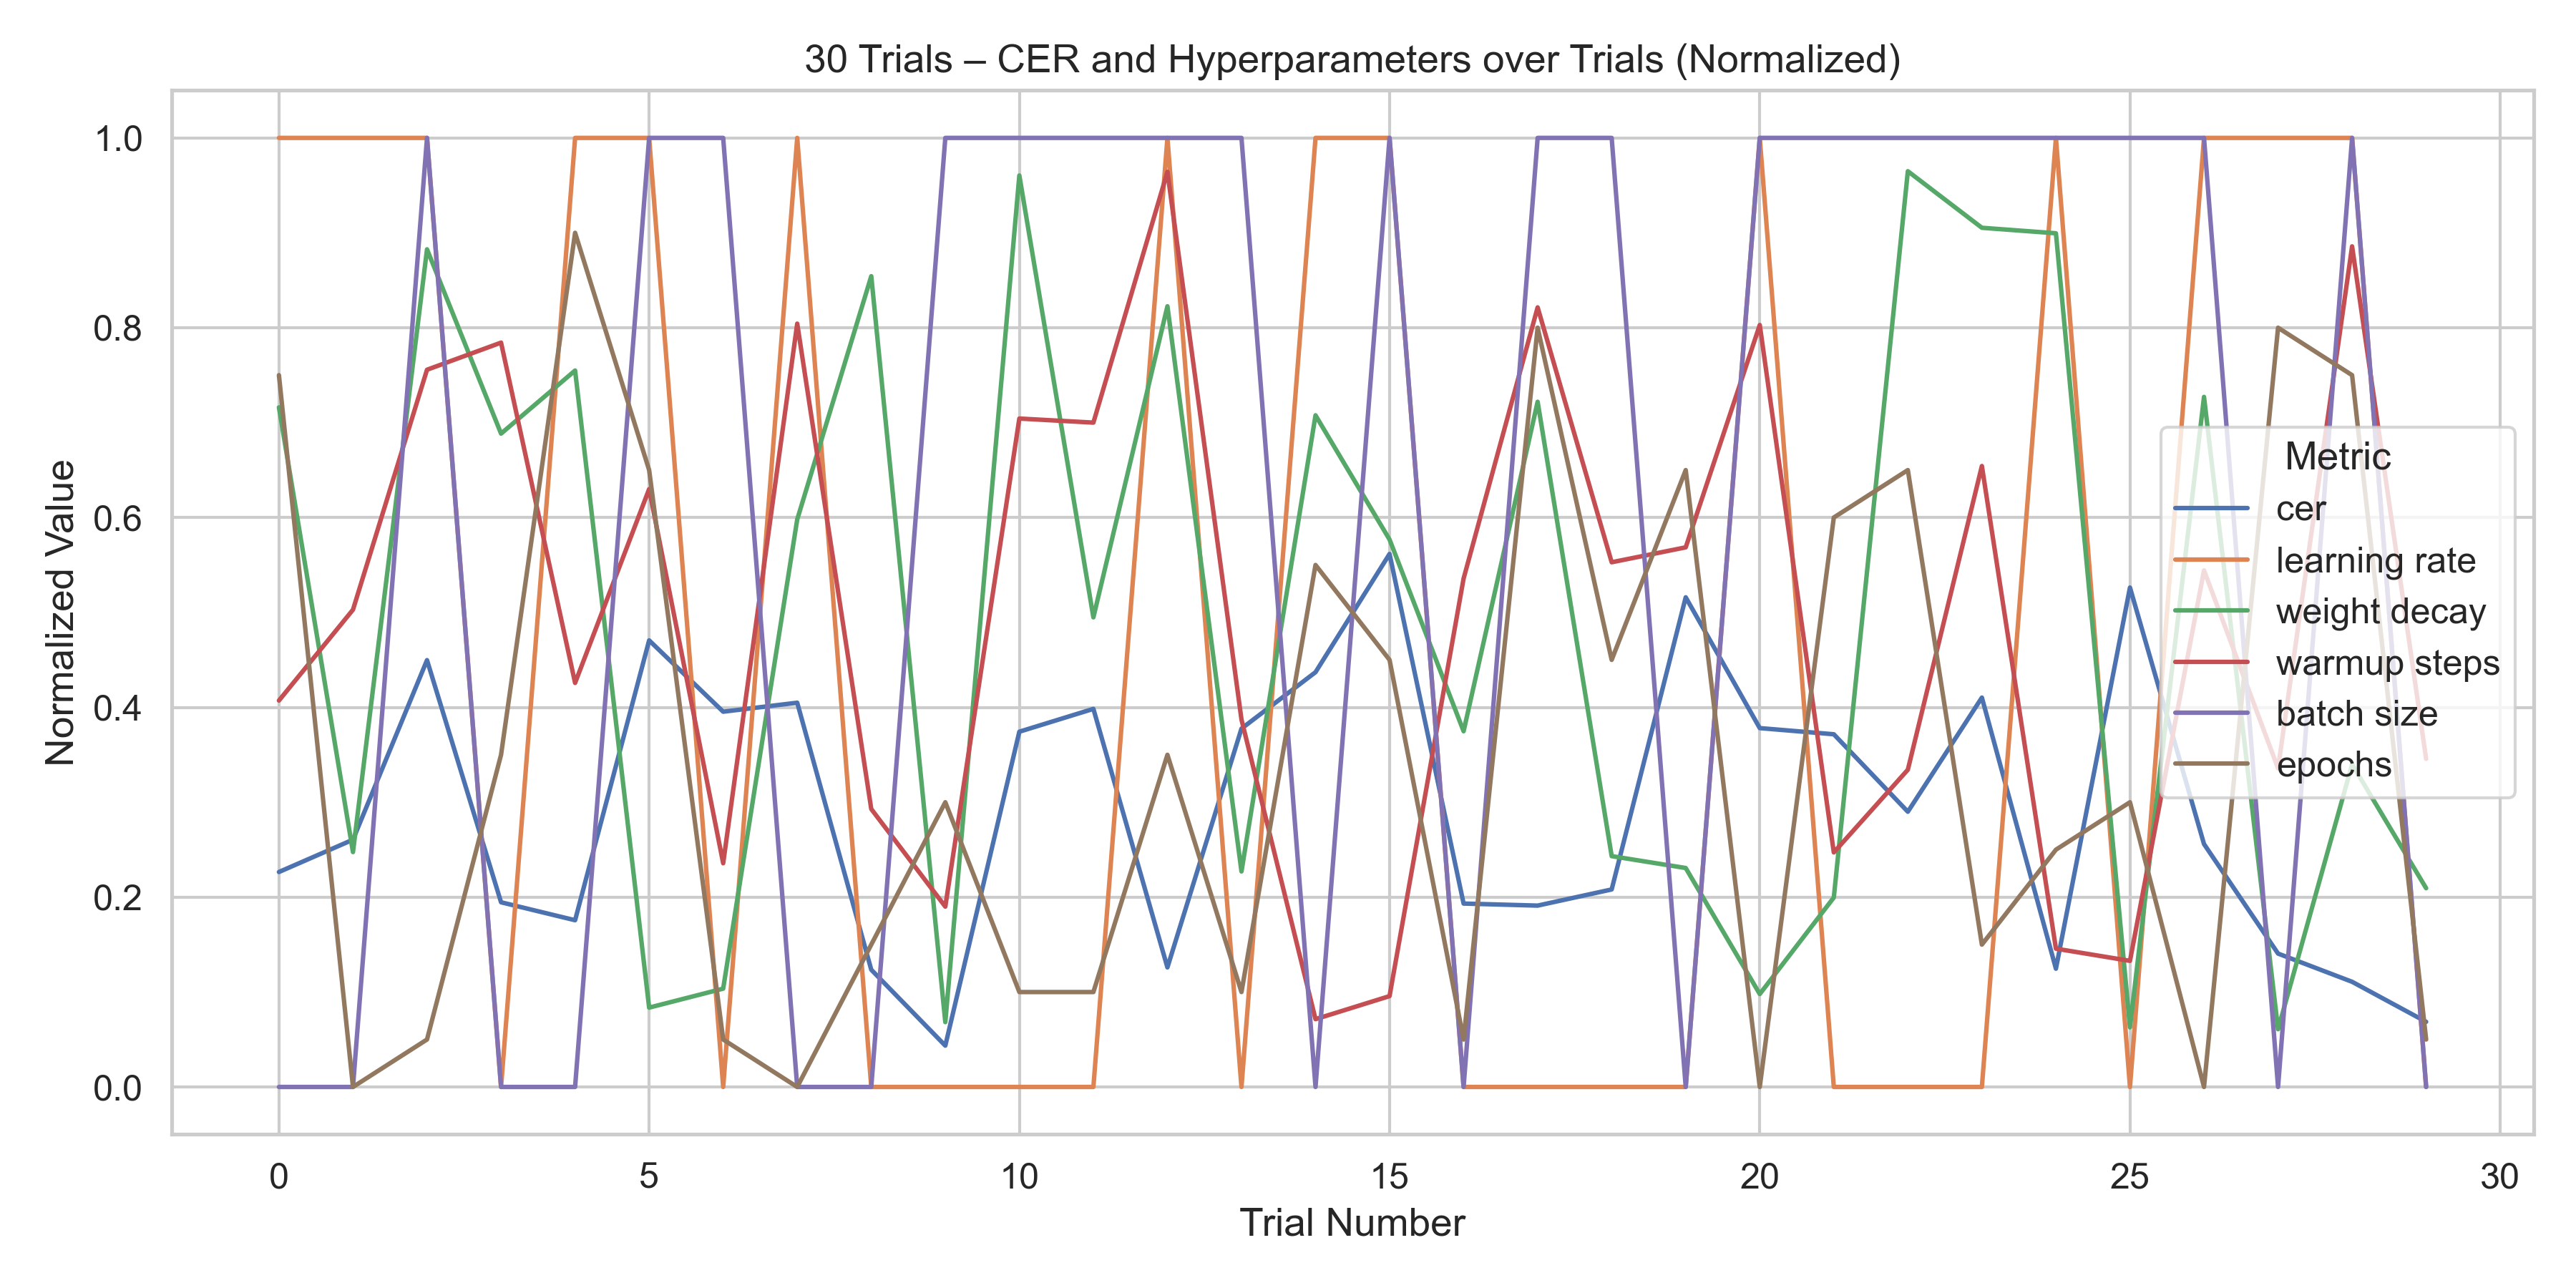
\includegraphics[width=\textwidth]{Figures/Chapter 4/trocr_metrics_scaled_30_Trials.png}
        \caption{30 Trials}
        \label{fig:trocr_cer_30}
    \end{subfigure}
    \vfill
    \begin{subfigure}[b]{0.7\textwidth}
        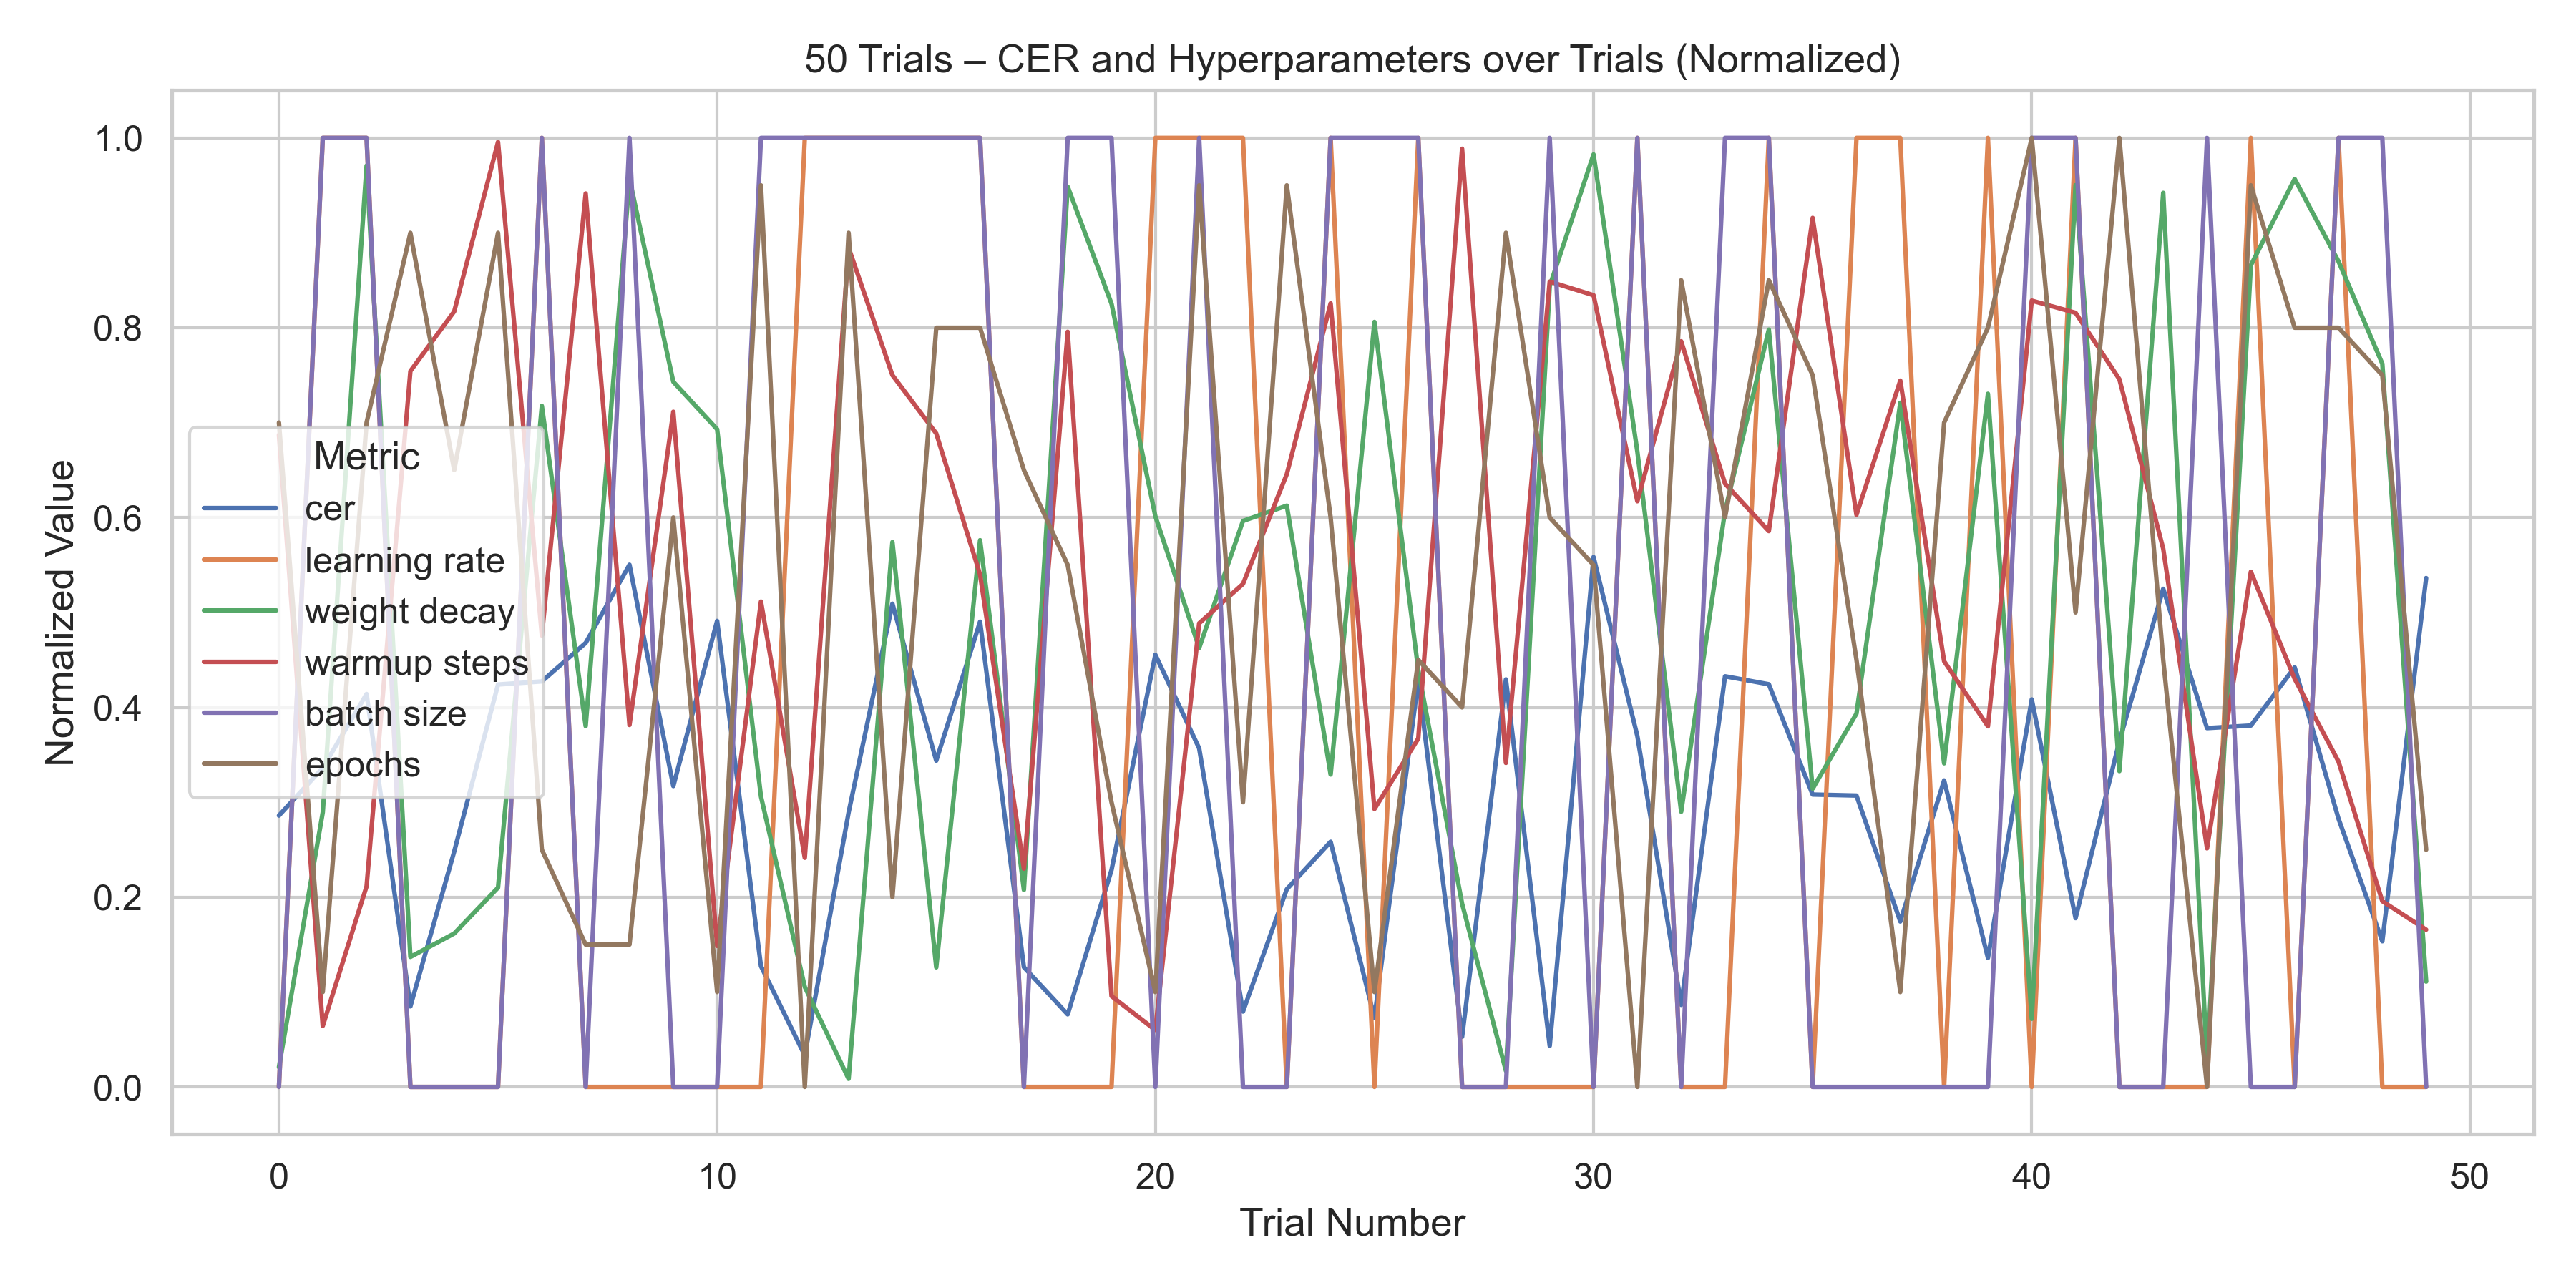
\includegraphics[width=\textwidth]{Figures/Chapter 4/trocr_metrics_scaled_50_Trials.png}
        \caption{50 Trials}
        \label{fig:trocr_cer_50}
    \end{subfigure}
    \vfill
    \begin{subfigure}[b]{0.7\textwidth}
        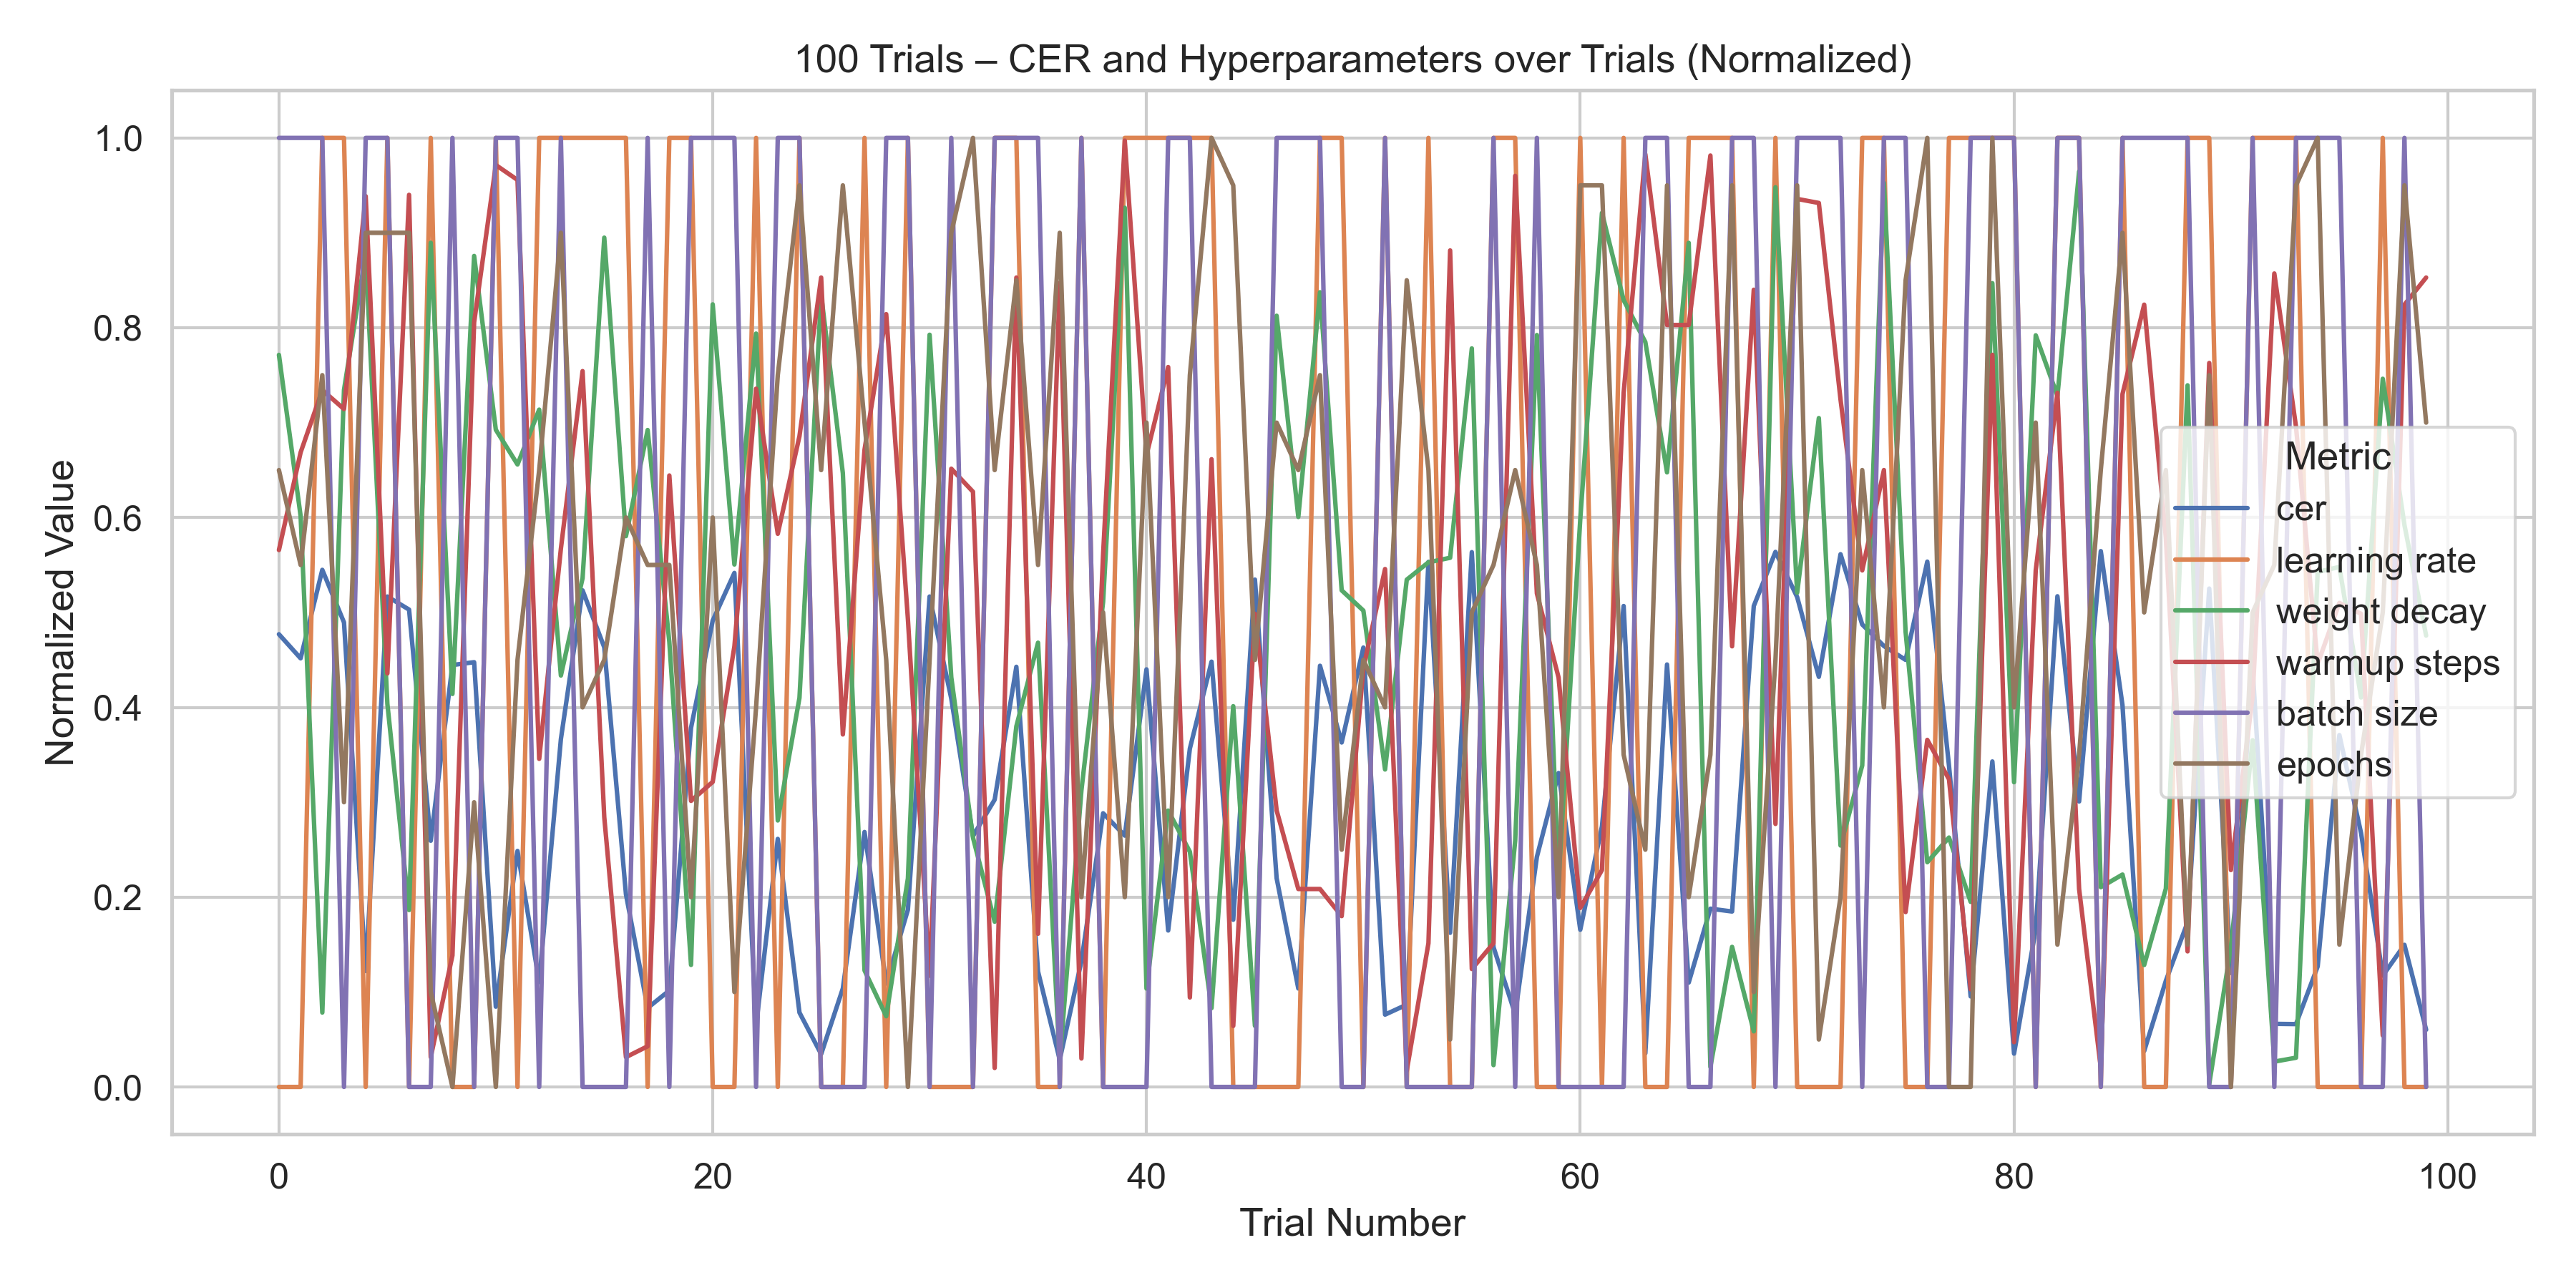
\includegraphics[width=\textwidth]{Figures/Chapter 4/trocr_metrics_scaled_100_Trials.png}
        \caption{100 Trials}
        \label{fig:trocr_cer_100}
    \end{subfigure}
    \caption{Evolution of CER and hyperparameter values across different trial counts in TrOCR.}
    \label{fig:trocr_cer_all_trials}
\end{figure}

Figure \ref{fig:trocr_cer_all_trials} visualizes the CER trajectory over the course of the trials. With 30 trials, Optuna explores the space broadly with higher variance in CER values. In the 50- and 100-trial settings, the optimization process achieves greater stability and reduced error variance, especially in the later trials, reflecting convergence towards optimal settings.

\subsubsection{Performance Summary and Observations}

The Optuna-based hyperparameter optimization for TrOCR revealed several key trends. First, increasing the number of trials led to marginal but consistent improvements across most performance metrics. The best Character Error Rate (CER) of 0.0406 is achieved in the 100-trial experiment, highlighting Optuna’s ability to refine parameter selection over time. Additionally, while the 30-trial configuration yielded a slightly lower average CER, the 100-trial run offered better accuracy and more stable validation losses, making it the most balanced configuration overall.

Analyzing the best hyperparameters (Table~\ref{tab:trocr_optuna_best_hyperparameters}) shows that lower learning rates ($\sim$1e-6), moderate weight decay, and a higher number of training epochs contributed positively to model performance. This emphasizes the need for gradual and regularized learning in TrOCR's fine-tuning process. The batch size of 8 in the top-performing trial suggests that smaller batches might help improve generalization in OCR tasks involving variable and noisy input data.

Overall, the experiments validate the effectiveness of hyperparameter tuning in enhancing TrOCR's performance and demonstrate the robustness of Optuna as an optimization tool in sequence-to-sequence vision-language models.

\clearpage
\section{HPO: Optimized OCR models for Medical Labels using \textbf{GA} }

This section presents the use of Genetic Algorithms (GA) for hyperparameter optimization of OCR models on medical label recognition.
Unlike Optuna, which uses adaptive sampling based on prior evaluations (e.g., TPE), GA explores the search space through evolutionary operations such as selection, crossover, and mutation.
\subsection{Principle steps for HPO with GA}

\begin{figure}[H]
    \centering
%    \begin{subfigure}[b]{\textwidth}
        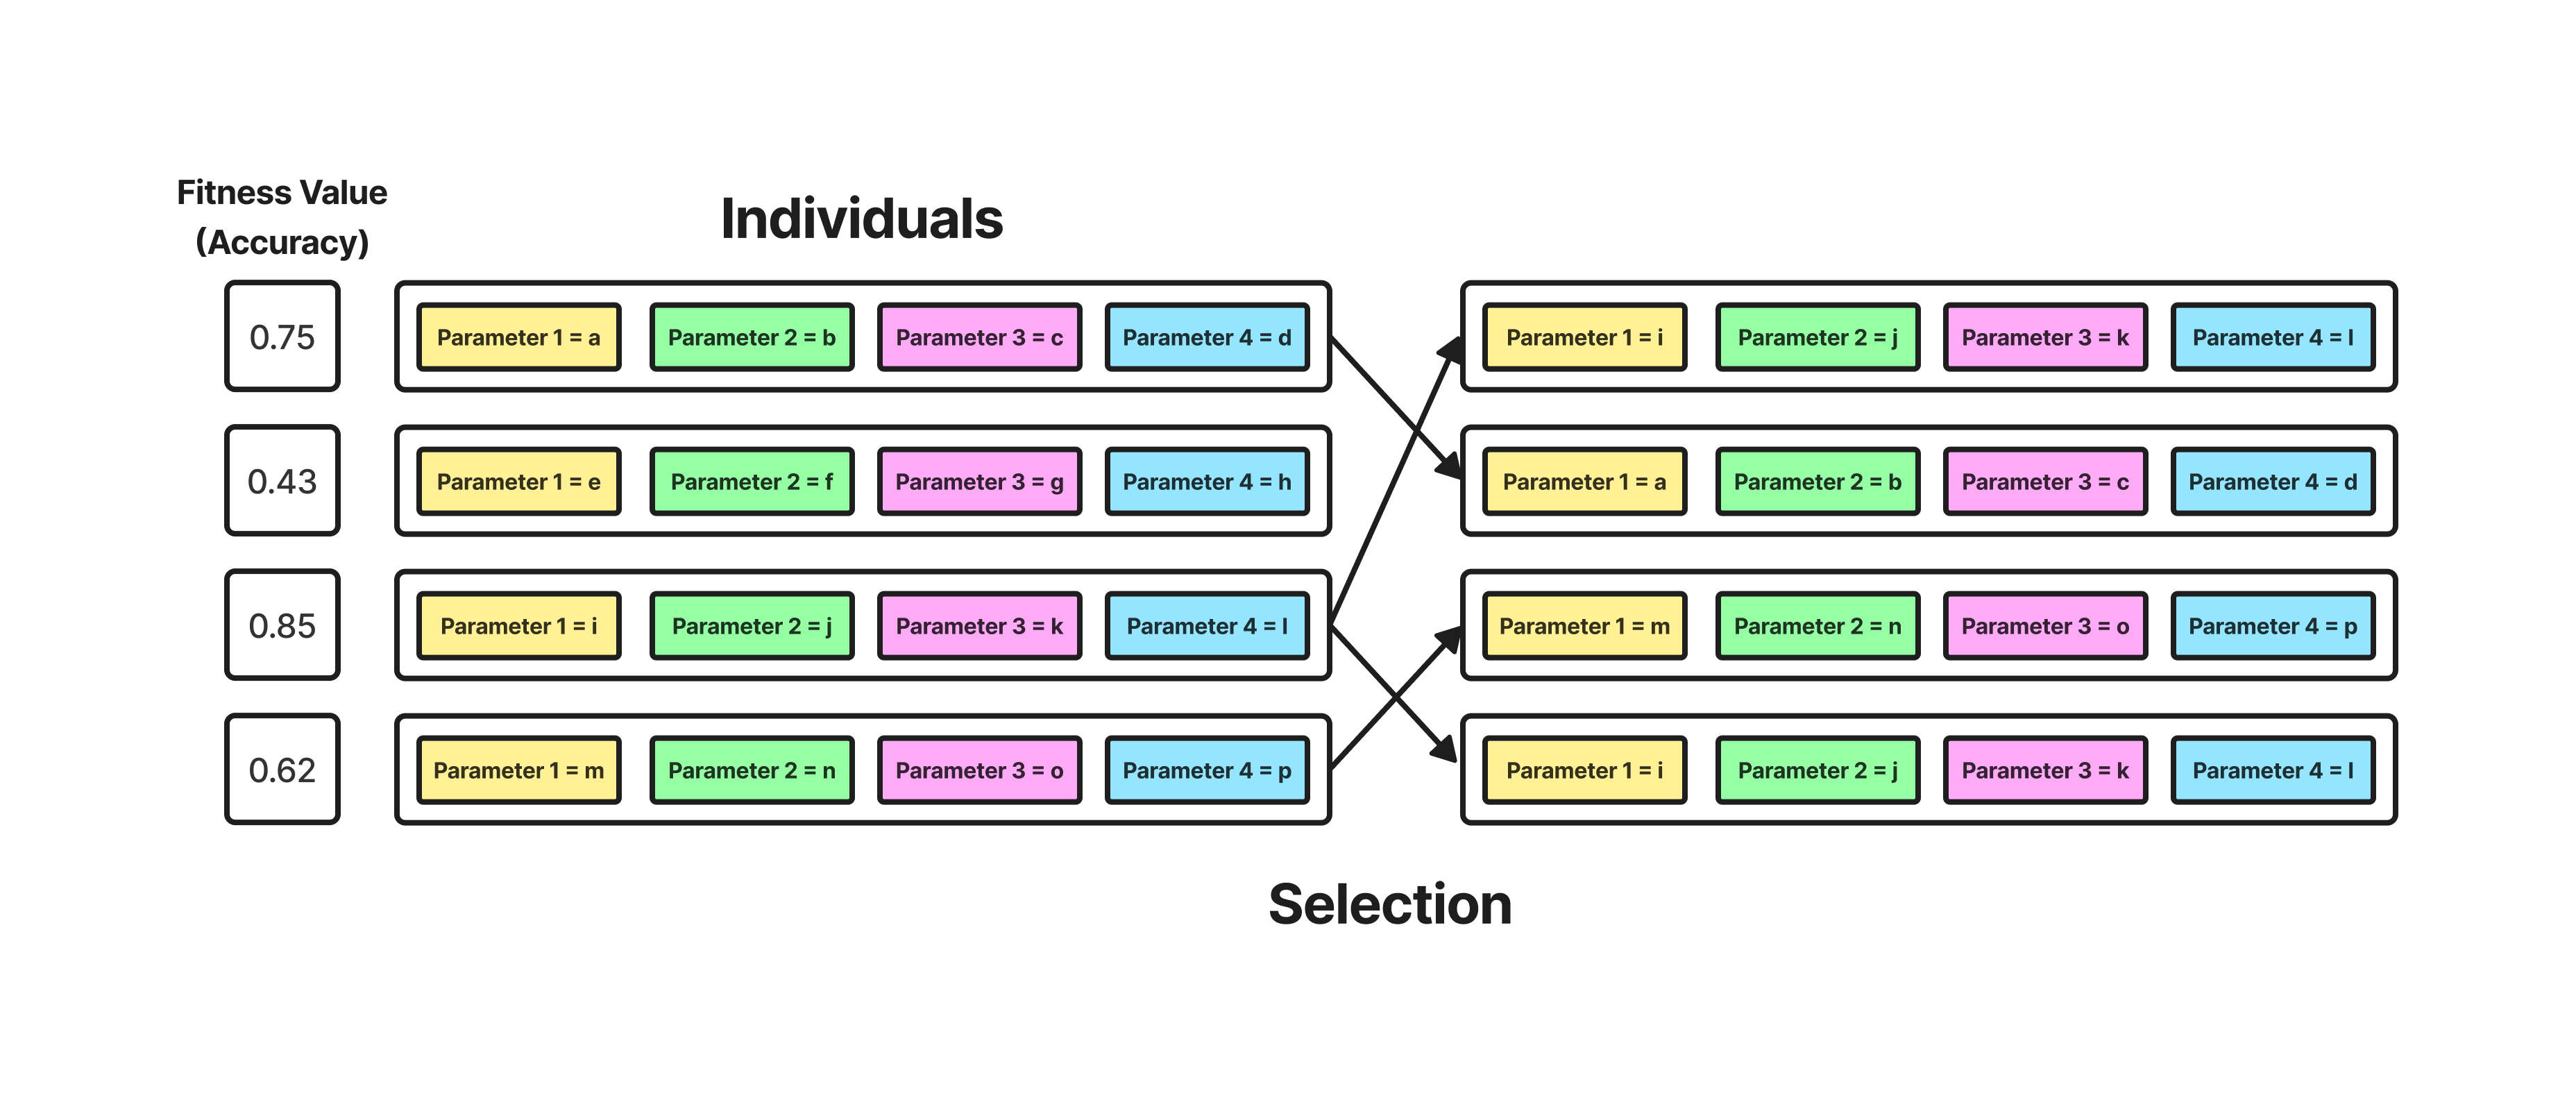
\includegraphics[width=\linewidth]{Figures/Chapter 4/ga_selection.png}
        \caption{Selection}
        \label{fig:selection}
%    \end{subfigure}
\end{figure}
    \vfill
\begin{figure}[H]
    \centering
%    \begin{subfigure}[b]{\textwidth}
        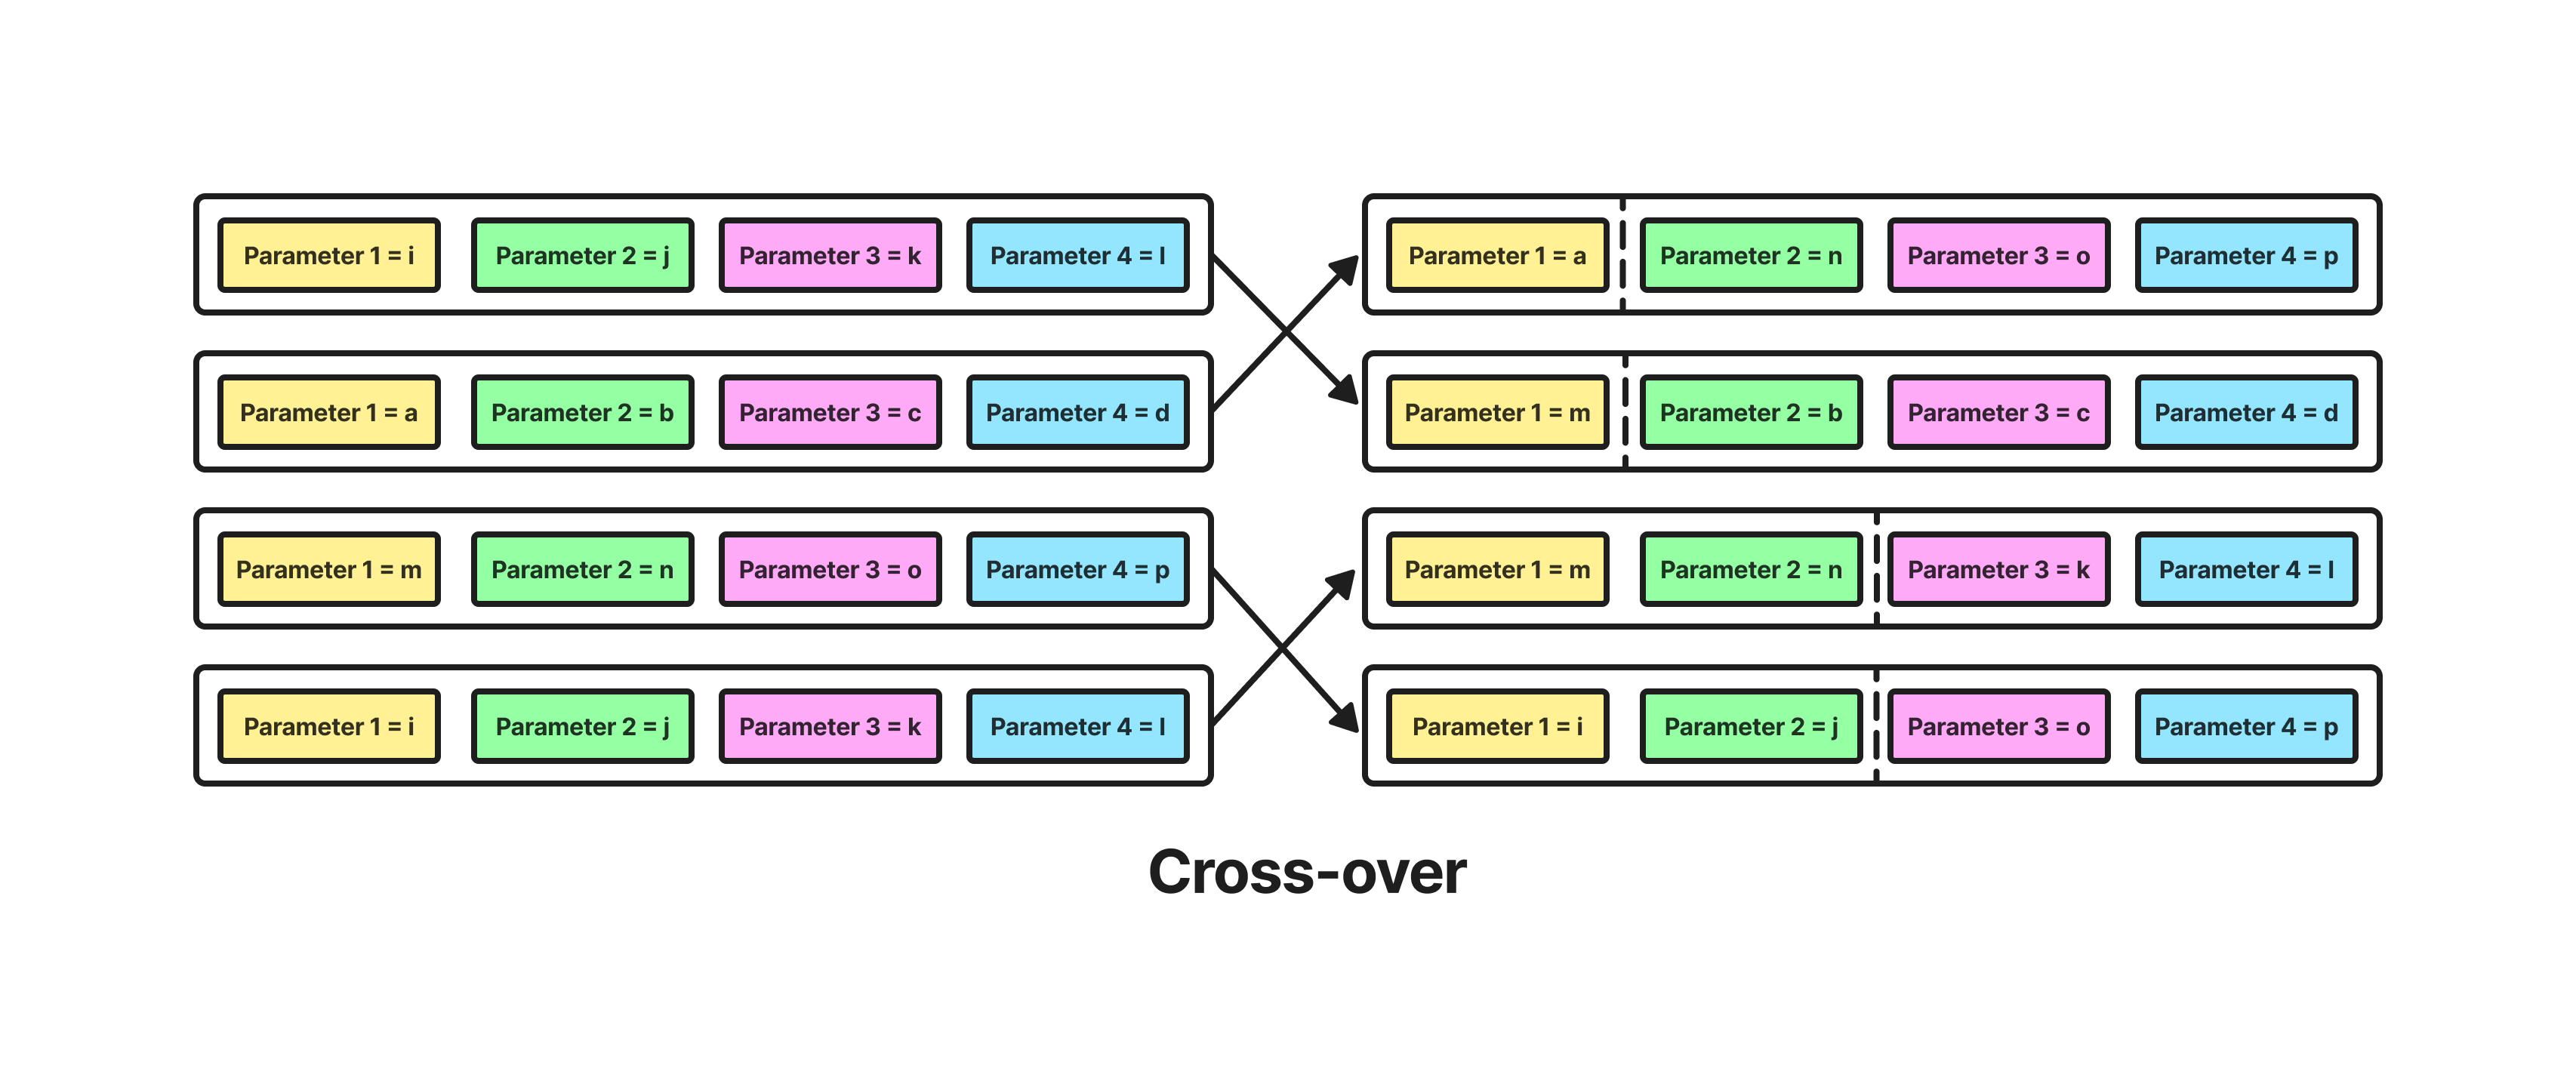
\includegraphics[width=\linewidth]{Figures/Chapter 4/ga_crossover.png}
        \caption{Crossover}
        \label{fig:crossover}
%    \end{subfigure}
\end{figure}

\begin{figure}[H]
    \centering
    %\begin{subfigure}[b]{\textwidth}
        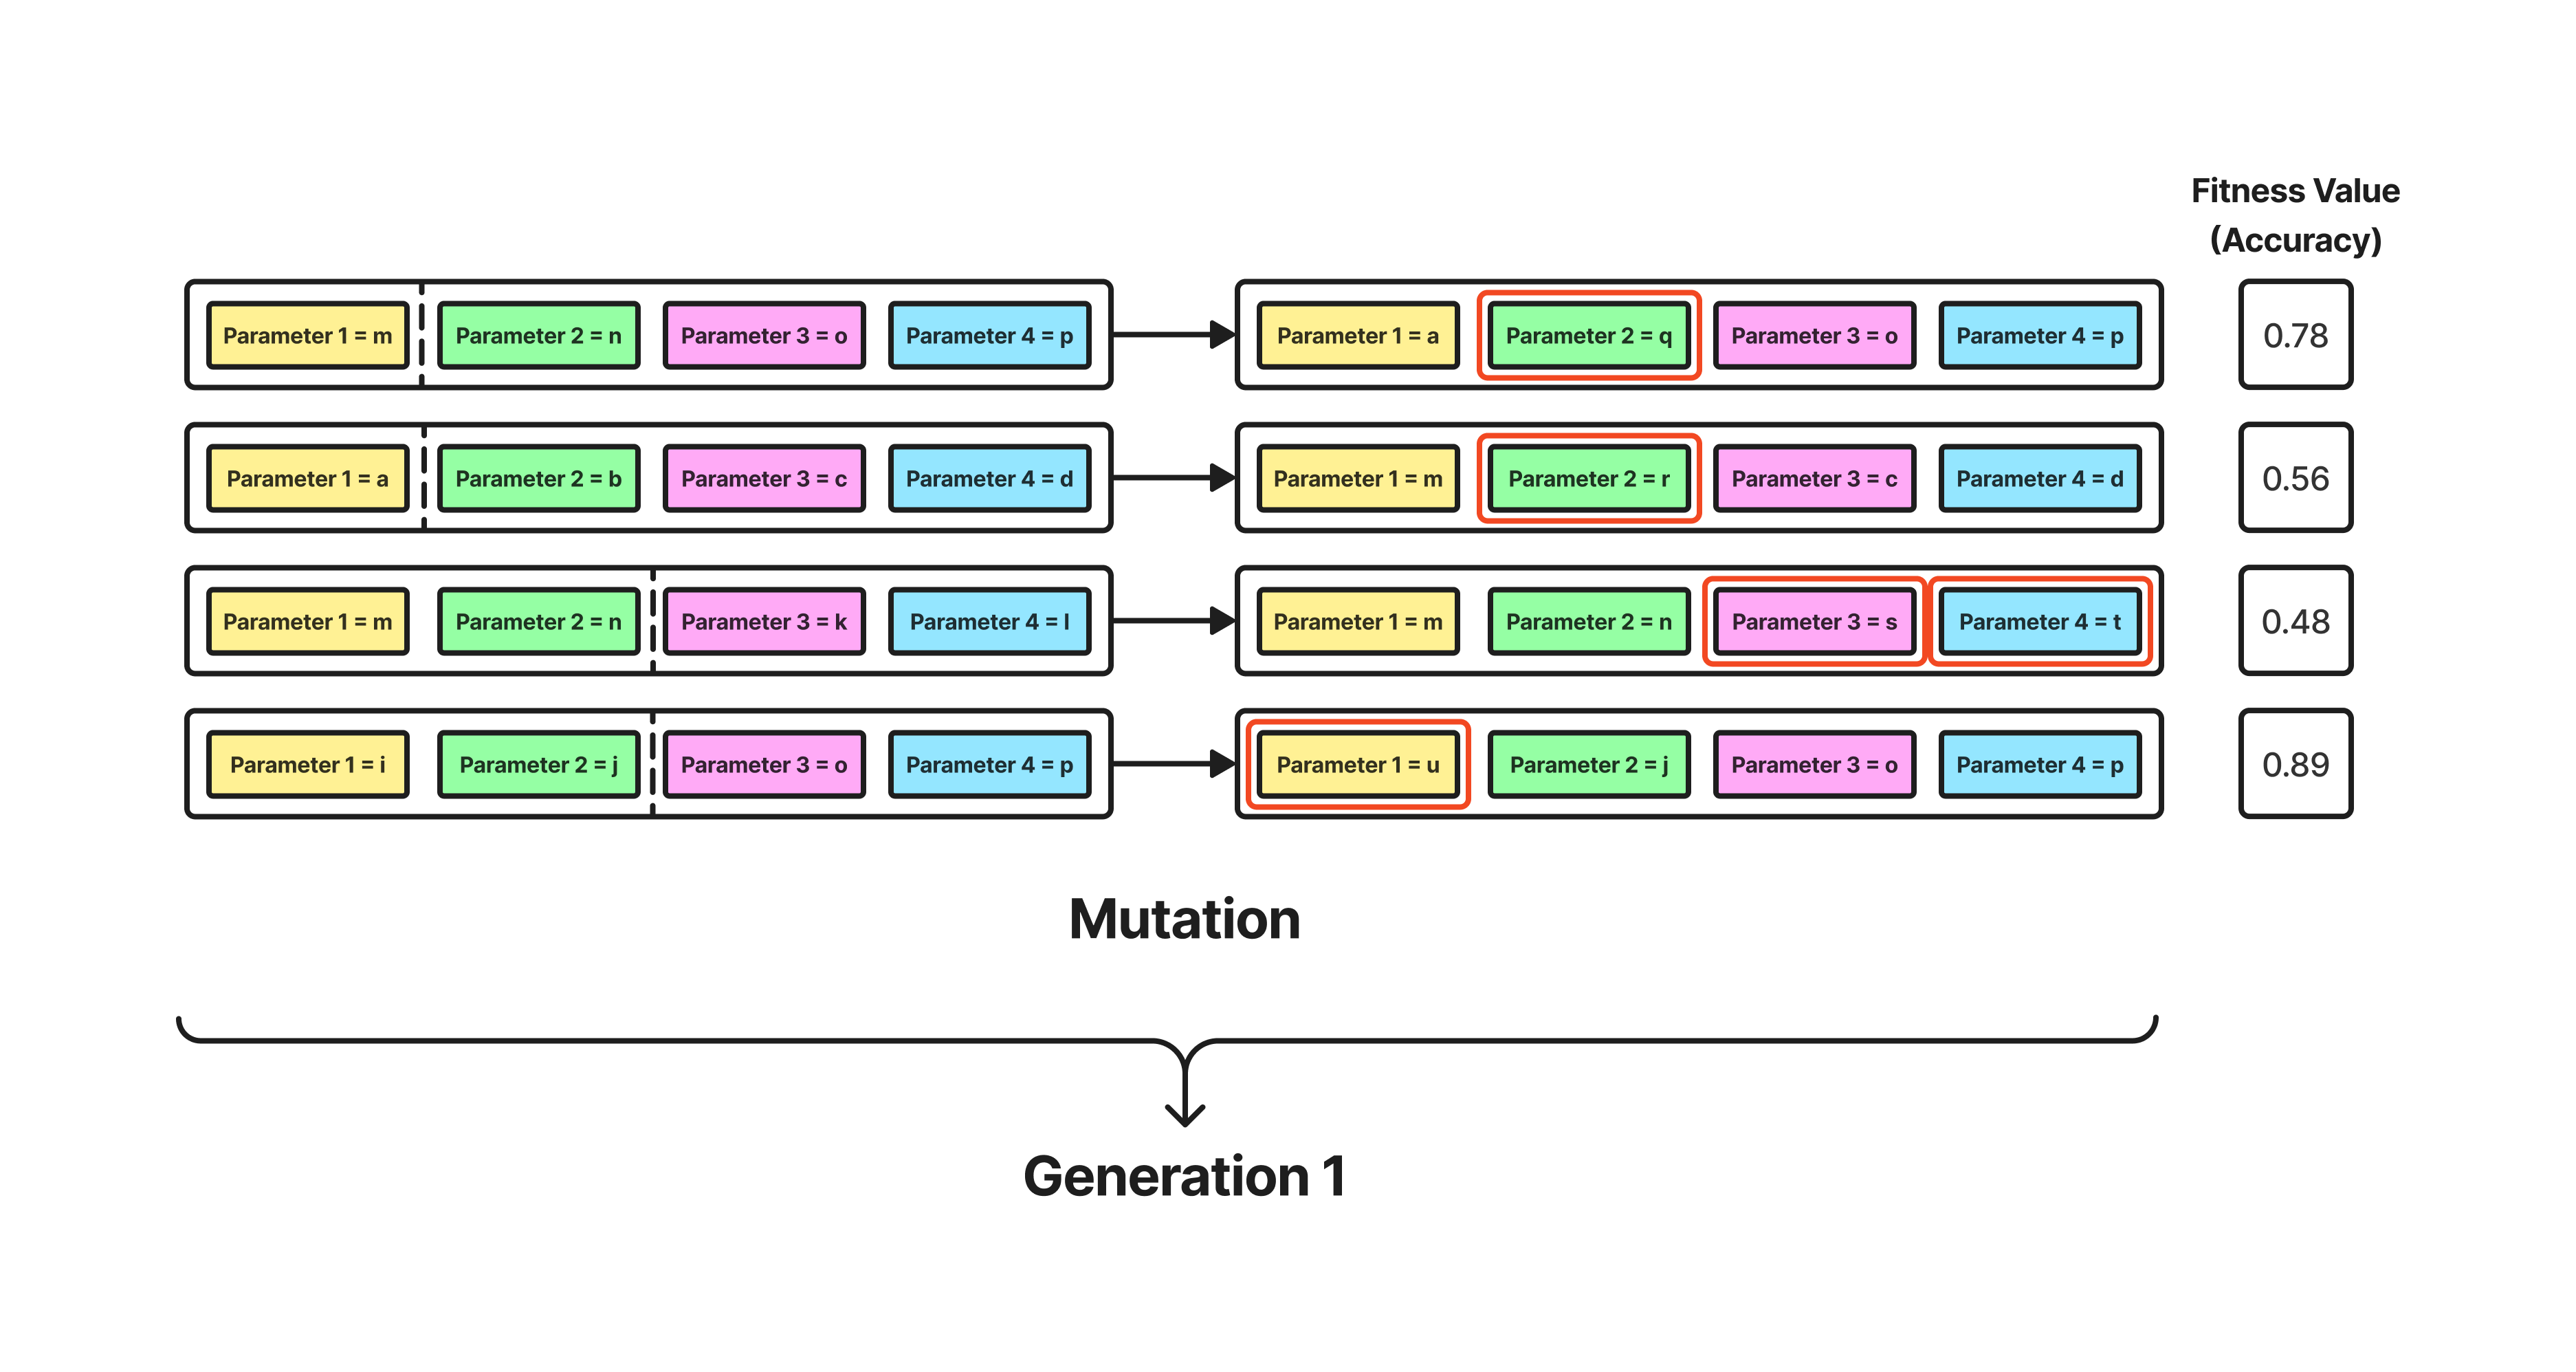
\includegraphics[width=\linewidth]{Figures/Chapter 4/ga_mutation.png}
        \caption{Mutation}
        \label{fig:mutation}
   % \end{subfigure}
\end{figure}

\begin{figure}
    \centering
   % \begin{subfigure}[b]{\textwidth}
        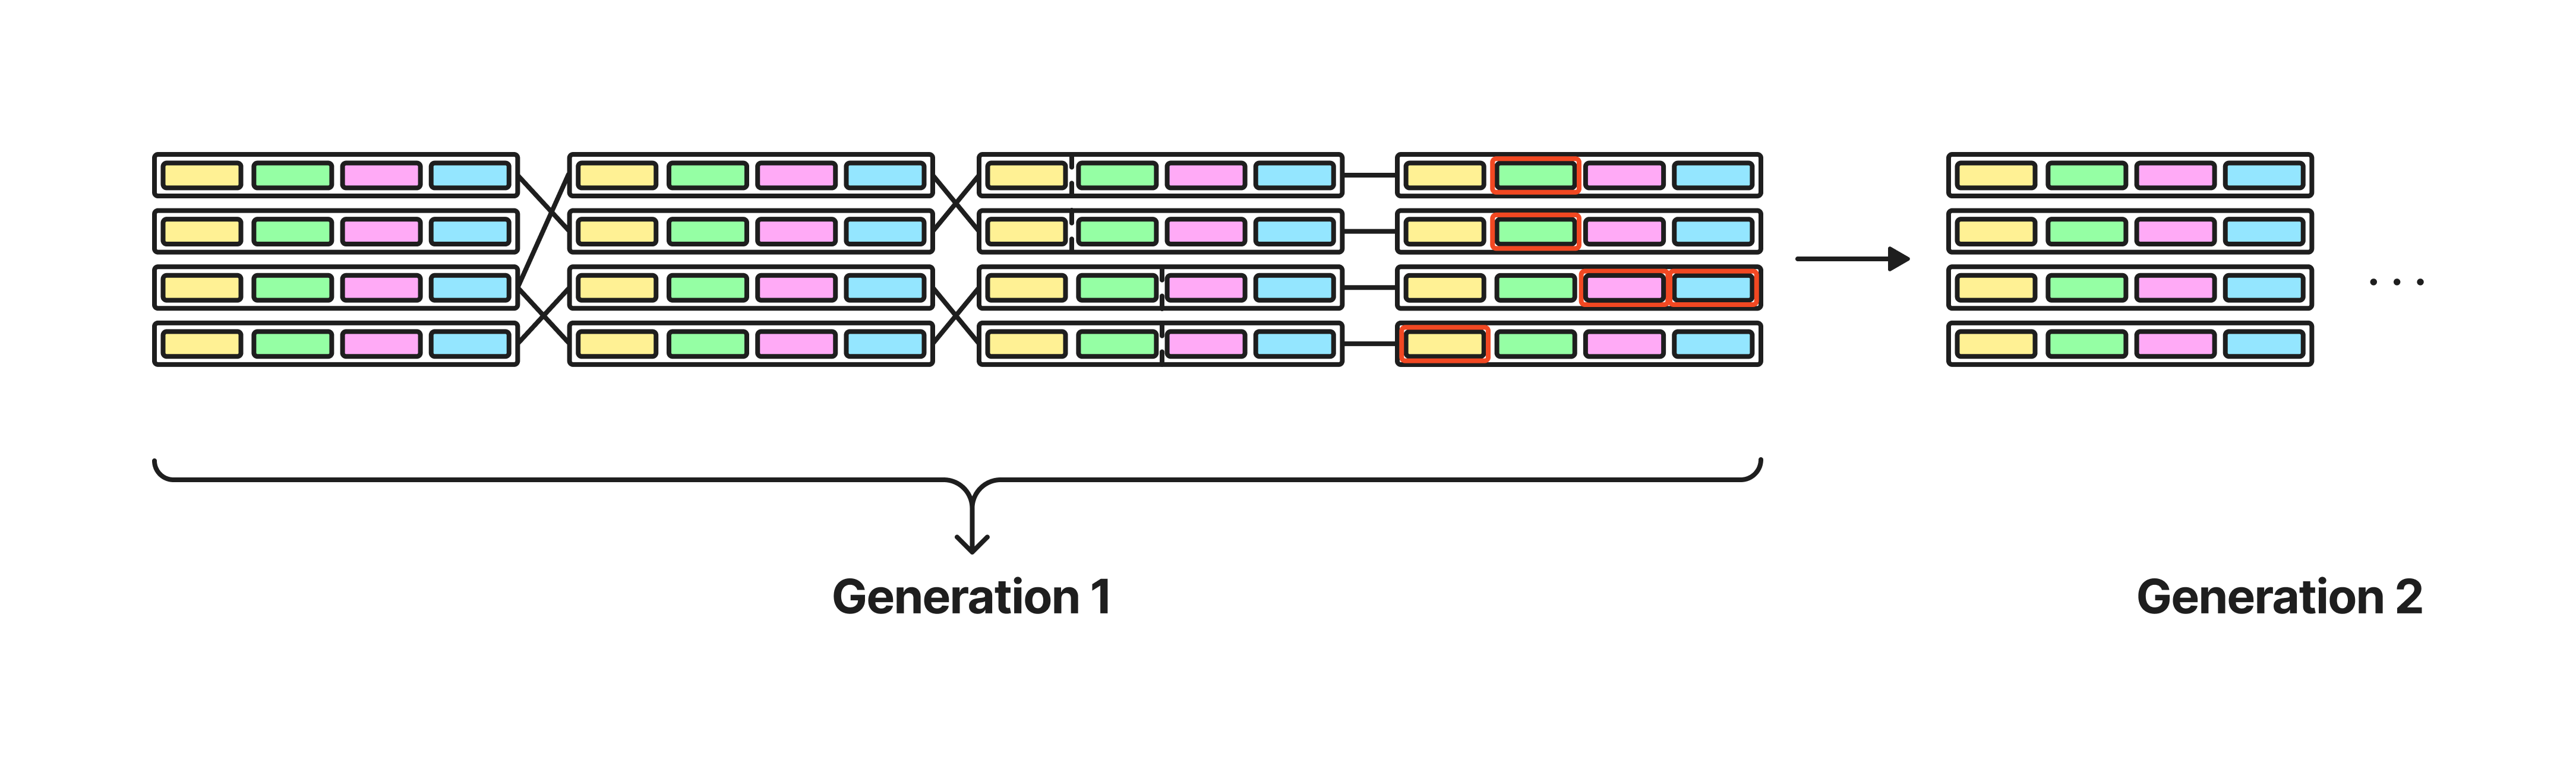
\includegraphics[width=\linewidth]{Figures/Chapter 4/ga_generation.png}
        \caption{Generations}
        \label{fig:generations}
%\end{subfigure}
    \caption{Principle Steps of HPO with GA}
    \label{fig:ga_part2}
\end{figure}

Figure \ref{fig:selection} – Selection:
This subfigure shows how individuals (i.e., hyperparameter sets) were selected from the population based on their fitness scores. In our case, the fitness score is inversely related to the Character Error Rate (CER), meaning that individuals with lower CER values had a higher probability of being selected. This figure demonstrates the emphasis on exploiting well-performing candidates while maintaining diversity in the gene pool.

Figure \ref{fig:crossover} – Crossover:
This subfigure depicts the crossover operation, where pairs of selected individuals exchange segments of their hyperparameter values to create offspring. This process introduces variability into the population, allowing the algorithm to explore new regions of the hyperparameter space. The figure illustrates how mixing parent traits can yield new candidate solutions that may outperform their predecessors.

Figure \ref{fig:mutation} – Mutation:
The mutation operation, shown in this subfigure, involves the random alteration of one or more hyperparameter values in an individual. This step prevents premature convergence and helps the population escape local minima by injecting novel traits into the gene pool. The figure highlights the sporadic nature of mutations and their distribution across individuals and generations.

Figure \ref{fig:generations} – Generations:
This final subfigure presents the evolution of the population over successive generations. It illustrates how the overall fitness (CER performance) of the population improves as the GA iterates. This progressive optimization demonstrates the algorithm's ability to converge toward an optimal or near-optimal set of hyperparameters through the interplay of selection, crossover, and mutation.

Together, these figures encapsulate the working mechanism of the Genetic Algorithm and how it incrementally improves the model's performance by evolving the population of hyperparameter sets through biologically inspired operations.

\subsubsection*{Selection and Crossover strategies used in this study}

In this study, several selection and crossover strategies have been explored to evaluate their impact on optimization performance and convergence speed. Selection techniques include:
\begin{itemize}
    \item \textbf{Tournament Selection (selTournament):} This widely used method selects individuals by holding "tournaments" among a subset of the population, choosing the best from each. It offers a good balance between exploration and exploitation, making it a natural initial choice.

    \item \textbf{NSGA-II Selection (selNSGA2):} Designed for multi-objective optimization, NSGA-II maintains a diverse set of high-quality solutions by ranking individuals using Pareto dominance and crowding distance. Although our problem is single-objective, NSGA-II is tested to potentially preserve genetic diversity and avoid premature convergence.

    \item \textbf{Roulette Wheel Selection (selRoulette):} This probabilistic selection favors fitter individuals proportionally but can sometimes lead to premature convergence due to loss of population diversity.
\end{itemize}
Additionally, crossover operators create offspring by combining genetic material from two parents, with different methods promoting varying degrees of exploration:
\begin{itemize}
\item \textbf{One-Point Crossover (cxOnePoint):} Exchanges gene segments after a randomly chosen point, preserving contiguous blocks of hyperparameters.

\item \textbf{Two-Point Crossover (cxTwoPoint):} Similar to one-point but swaps segments between two points, increasing genetic variation.

\item \textbf{Blend Crossover (cxBlend):} Generates offspring by blending continuous-valued genes of parents, suited for floating-point hyperparameters like learning rate and momentum terms.
\end{itemize}

%These selection and crossover strategies were tested to evaluate their impact on optimization performance and convergence speed.



\subsection{TesseractOCR Hyperparameter optimization: Description and experimental results}

This section presents the methodology and results of applying GA to optimize TesseractOCR's hyperparameters. The optimization focused on the same Hyperparameters used by Optuna (table \ref{tab:tesseract_hyperparameters}) and network architecture settings, targeting improved recognition accuracy for Medical Labels. Through systematic experimentation with different selection and crossover operators, we identified configurations that
significantly enhance the model's performance while maintaining computational efficiency.
\begin{comment}

\subsubsection*{Experimental Setup}

GA for optimizing Tesseract OCR training is built using the DEAP framework (Distributed Evolutionary Algorithms in Python). This pipeline aimed to automate the search for optimal LSTM training parameters for fine-tuning a pre-trained Tesseract model on a French ground-truth dataset.
    
%The population consisted of individuals representing various configurations, including learning rate, momentum, number of iterations, and the network architecture path. Training is executed using the lstmtraining.exe binary, with output models saved to a dedicated directory. The selection method used is selTournament, and crossover is implemented using cxOnePoint for its simplicity in combining parent solutions. Mutation is performed with a custom function to ensure all hyperparameters remained within valid ranges, and specific care is taken to constrain categorical variables.

%Each individual is evaluated by running the Tesseract LSTM training command via a subprocess call. The output logs were parsed using regular expressions to extract the final training loss. In case of training failure or errors in execution, the corresponding individuals were penalized with an infinite fitness score.

%The model used as a starting point is fra.lstm, with training data consisting of pre-labeled images and box files. Configuration files were auto-generated and dynamically updated to reflect the evolving parameters.

%\subsubsection*{Evaluation Strategy}

The fitness function returns the final reported training loss as the primary optimization objective. All training logs are parsed to compute performance metrics, and results are stored in a logbook for visualization using Seaborn and Matplotlib. A Hall of Fame mechanism tracked the most optimal configuration across all generations, and the best hyperparameter set is exported for future reproducibility and deployment.

The goal of this setup is to reduce manual trial-and-error and discover configurations that consistently improve OCR accuracy on low-quality document scans, enabling robust fine-tuning of Tesseract's recognition of the Algerian Medical labels.
\end{comment}


\subsubsection{Experimental Setup}

The GA optimization pipeline is implemented using the DEAP framework (Distributed Evolutionary Algorithms in Python). The pipeline automates the tuning of LSTM-based training parameters used during the fine-tuning of a pre-trained Tesseract model. The fitness function evaluates configurations based on final training loss, which acts as a proxy for convergence and model quality. All logs are parsed for metric extraction, and results are recorded in a logbook for visualization with Seaborn and Matplotlib. Additionally, a Hall of Fame mechanism is used to retain the top-performing individuals across generations for reproducibility and further experimentation.

Initially, we began the optimization using the Tournament selection method combined with three different crossover strategies: OnePoint, TwoPoint, and Blend. Among these, the Blend crossover consistently produced better CER outcomes, prompting us to adopt it for further experiments. After establishing Blend as the preferred crossover strategy, we explored alternative selection methods, including NSGA2 and Roulette, to compare their impact on performance.

We also evaluated the effect of increasing the number of generations. While early experiments were conducted with 10 generations, we later expanded this to 15 to assess whether additional evolutionary steps would yield further improvements or whether performance plateaus after a certain point. These incremental adjustments provided deeper insights into how selection pressure and search space exploration affect model tuning in the context of low-quality, real-world medical label recognition.


\begin{comment}
\begin{table}[H]
\centering
\caption{Tesseract parameters values of best individuals from each GA configuration}
\resizebox{\textwidth}{!}{
\begin{tabular}{llccccc}
\hline
\textbf{Selection} & \textbf{Crossover} & \textbf{Generations} & \textbf{Best Individual} & \textbf{Val Accuracy} & \textbf{Accuracy} & \textbf{CER} \\
\hline
selNSGA2 & cxBlend & 10  & Gen1\_Ind6 & 60.520 & 71.300 & 0.7224 \\
selRoulette & cxBlend & 10  & Gen9\_Ind6 & 62.060 & 73.480 & 0.0758 \\
selTournament & cxBlend & 10  & Gen6\_Ind2 & \textbf{66.720} & \textbf{78.470} & \textbf{0.0627} \\
selTournament & cxBlend & 15  & Gen9\_Ind6 & 64.040 & 75.610 & 0.0659 \\
selTournament & cxOnePoint & 10  & Gen2\_Ind7 & 64.760 & 74.020 & 0.1184 \\
selTournament & cxTwoPoint & 10  & Gen1\_Ind3 & 65.850 & 74.070 & 0.1087 \\
\hline
\end{tabular}}
\label{tab:ga_tesseract_performance}
\end{table}

\begin{table}[H]
\centering
\caption{Average metrics for each GA-based Tesseract configuration}
\begin{tabular}{lccc}
\hline
\textbf{Experiment} & \textbf{Val Accuracy (\%)} & \textbf{Train Accuracy (\%)} & \textbf{CER} \\
\hline
SelNSGA2\_cxBlend\_10Gen & 62.00 & 70.16 & 0.0824 \\
SelRoulette\_cxBlend\_10Gen & 63.42 & 71.78 & 0.0771 \\
SelTournament\_cxBlend\_10Gen & 67.00 & 77.45 & 0.0653 \\
SelTournament\_cxBlend\_15Gen & 64.13 & 72.92 & 0.0756 \\
SelTournament\_cxOnePoint\_10Gen & 65.02 & 74.64 & 0.0724 \\
SelTournament\_cxTwoPoint\_10Gen & 64.98 & 74.50 & 0.0730 \\
\hline
\end{tabular}
\label{tab:ga_tesseract_config_results}
\end{table}
\end{comment}



\subsubsection{Results Summary}
This section will summarize the results of our experiments and will give a general insight on the results of our findings.


\begin{table}[H]
\centering
\caption{Crossover Strategy Comparison using Tournament Selection (10 Generations)}
\begin{tabular}{lcccccc}
\hline
\textbf{Crossover} & \multicolumn{2}{c}{\textbf{Val Accuracy (\%)}} & \multicolumn{2}{c}{\textbf{Accuracy (\%)}} & \multicolumn{2}{c}{\textbf{CER}} \\
 & Best & Avg & Best & Avg & Best & Avg \\
\hline
Blend      & \textbf{66.72} & \textbf{67.00} & \textbf{78.47} & \textbf{77.45} & \textbf{0.0627} & \textbf{0.0653} \\
OnePoint   & 64.76 & 65.02 & 74.02 & 74.64 & 0.1184 & 0.0724 \\
TwoPoint   & 65.85 & 64.98 & 74.07 & 74.50 & 0.1087 & 0.0730 \\
\hline
\end{tabular}
\label{tab:ga_tesseract_crossover_comparison}
\end{table}

\begin{table}[H]
\centering
\caption{Selection Method Comparison using Blend Crossover (10 Generations)}
\begin{tabular}{lcccccc}
\hline
\textbf{Selection} & \multicolumn{2}{c}{\textbf{Val Accuracy (\%)}} & \multicolumn{2}{c}{\textbf{Accuracy (\%)}} & \multicolumn{2}{c}{\textbf{CER}} \\
 & Best & Avg & Best & Avg & Best & Avg \\
\hline
NSGA2      & 60.52 & 62.00 & 71.30 & 70.16 & 0.7224 & 0.0824 \\
Roulette   & 62.06 & 63.42 & 73.48 & 71.78 & 0.0758 & 0.0771 \\
Tournament & \textbf{66.72} & \textbf{67.00} & \textbf{78.47} & \textbf{77.45} & \textbf{0.0627} & \textbf{0.0653} \\
\hline
\end{tabular}
\label{tab:ga_tesseract_selection_comparison}
\end{table}

\begin{table}[H]
\centering
\caption{Effect of Generation Number using Tournament Selection and Blend Crossover}
\begin{tabular}{lcccccc}
\hline
\textbf{Generations} & \multicolumn{2}{c}{\textbf{Val Accuracy (\%)}} & \multicolumn{2}{c}{\textbf{Accuracy (\%)}} & \multicolumn{2}{c}{\textbf{CER}} \\
 & Best & Avg & Best & Avg & Best & Avg \\
\hline
10  & \textbf{66.72} & \textbf{67.00} & \textbf{78.47} & \textbf{77.45} & \textbf{0.0627} & \textbf{0.0653} \\
15  & 64.04 & 64.13 & 75.61 & 72.92 & 0.0659 & 0.0756 \\
\hline
\end{tabular}
\label{tab:ga_tesseract_generation_comparison}
\end{table}

\begin{table}[H]
\centering
\caption{Tesseract Hyperparameters of best individuals from each GA configuration}
\begin{tabular}{cccccc}
\hline
\textbf{Best Individual} & \textbf{lr} & \textbf{max\_iter} & \textbf{adam\_beta} & \textbf{momentum} & \textbf{weight\_range} \\
\hline
Gen1\_Ind6 & 0.07527 & 1097 & 0.9872 & 0.2270 & 0.4490 \\
Gen9\_Ind6 & 0.06259 & 1405 & 0.9610 & 0.8090 & 0.1930 \\
Gen6\_Ind2 & 0.05427 & 663 & 0.9585 & 0.3290 & 0.1120 \\
Gen9\_Ind6 & 0.06259 & 1405 & 0.9610 & 0.8090 & 0.1930 \\
Gen2\_Ind7 & 0.03798 & 1239 & 0.9514 & 0.7910 & 0.2920 \\
Gen1\_Ind3 & 0.05651 & 910 & 0.9494 & 0.7170 & 0.1050 \\
\hline
\end{tabular}
\label{tab:ga_tesseract_hyperparams}
\end{table}

\begin{figure}[H]
\centering
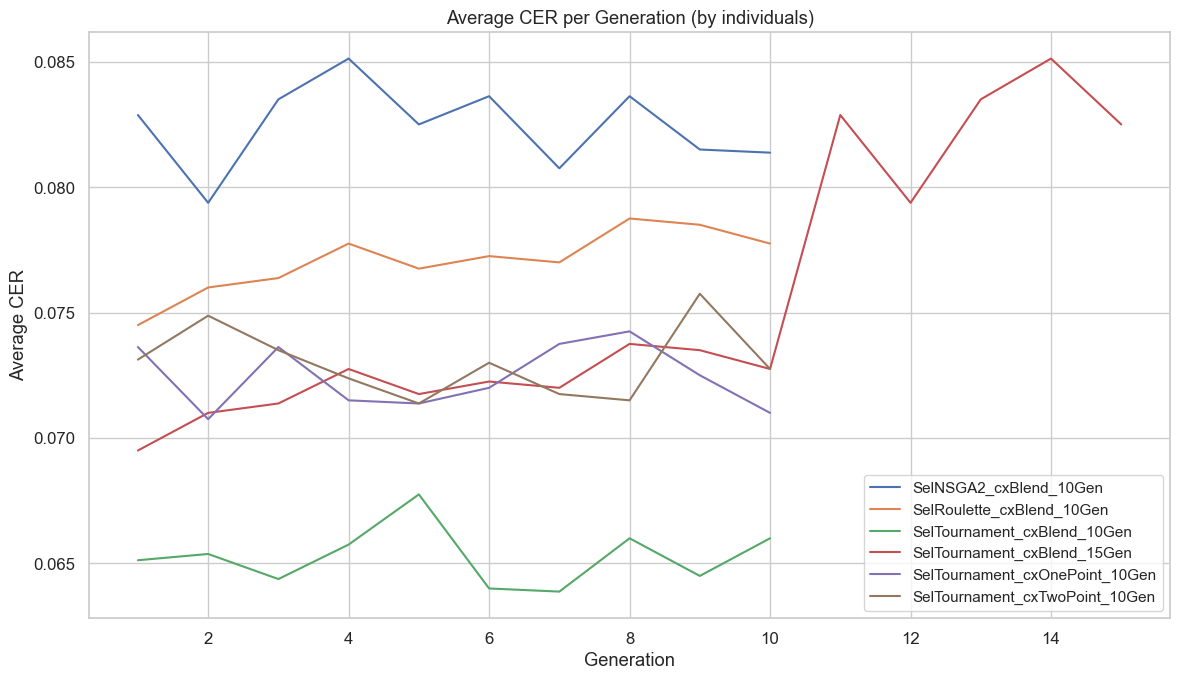
\includegraphics[width=0.70\textwidth]{Figures/Chapter 4/tesseract_ga_average_cer.png}
\caption{Tesseract Average CER over generations in each Expirement}
\label{fig:tesseractocraveragecer}
\end{figure}

Table~\ref{tab:ga_tesseract_crossover_comparison} shows the impact of different crossover strategies (Blend, OnePoint, TwoPoint) using the Tournament selection method with 10 generations. The Blend crossover clearly outperforms the others, yielding the lowest best CER (0.0627) and the best average CER (0.0653). Both OnePoint and TwoPoint showed significantly higher error rates, indicating that Blend enables better exploration and preservation of beneficial traits across generations.


Table~\ref{tab:ga_tesseract_selection_comparison} compares different selection strategies (NSGA2, Roulette, Tournament), all paired with the Blend crossover over 10 generations. Tournament selection stands out as the most effective method, achieving both the best and average CER values (0.0627 and 0.0653, respectively). NSGA2 performed notably worse in this setup, with a best CER of 0.7224, suggesting that Tournament selection provides stronger selection pressure, which is more suitable for this task.


Table~\ref{tab:ga_tesseract_generation_comparison} analyzes the impact of increasing the number of generations from 10 to 15 using Tournament selection and Blend crossover. The 10-generation run yielded better CER results, both best and average (0.0627 and 0.0653), compared to the 15-generation run (0.0659 and 0.0756). This suggests that additional generations do not necessarily lead to better performance and that 10 generations may be sufficient for convergence in this problem space.

Table~\ref{tab:ga_tesseract_hyperparams} lists the hyperparameter values of the best individuals from each configuration. The best results are generally associated with moderate learning rates (around 0.05–0.06), stable momentum values (ranging from 0.22 to 0.80), and consistent use of adam\_beta near 0.95–0.99. These patterns suggest that balanced settings, rather than extreme values, tend to yield better model performance.


%Figure \ref{fig:tesseractocraveragecer} Shows the average CER reduction over generations for each experiment. It shows that most experiments were  Most configurations converge quickly within the first 6–8 generations.

Figure~\ref{fig:tesseractocraveragecer} presents the evolution of average CER across generations for various GA configurations applied to TesseractOCR. The configuration using Tournament selection with Blend crossover over 10 generations consistently achieved the lowest and most stable CER, indicating effective convergence. In contrast, NSGA2 and Roulette showed higher error rates with less stability. The setup with 15 generations showed increased fluctuations after generation 10, suggesting that extending the run does not necessarily yield better results. Overall, the plot confirms that 10 generations with Tournament + Blend is the most reliable configuration.



\subsubsection{Visual Analysis}


\begin{figure}[H]
\centering
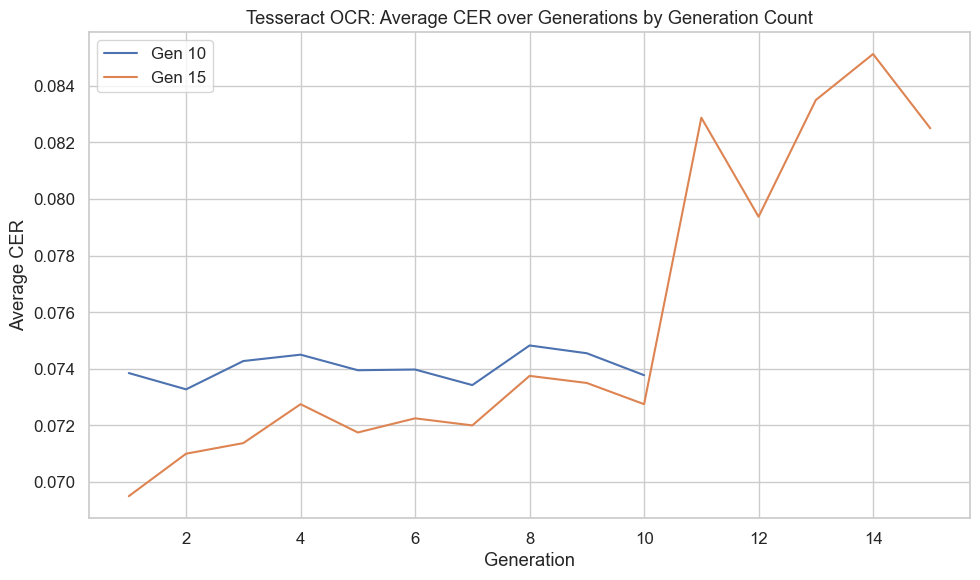
\includegraphics[width=0.70\textwidth]{Figures/Chapter 4/tesseract_impact_of_generation.png}
\caption{Impact of Number of Generation on CER in Tesseract (Average)}
\label{fig:Tesseractimpactofgen}
\end{figure}

Figure \ref{fig:Tesseractimpactofgen} Highlights how increasing the number of generations from 10 to 15 slightly improves CER in some cases, but with diminishing returns.

\begin{figure}[H]
\centering
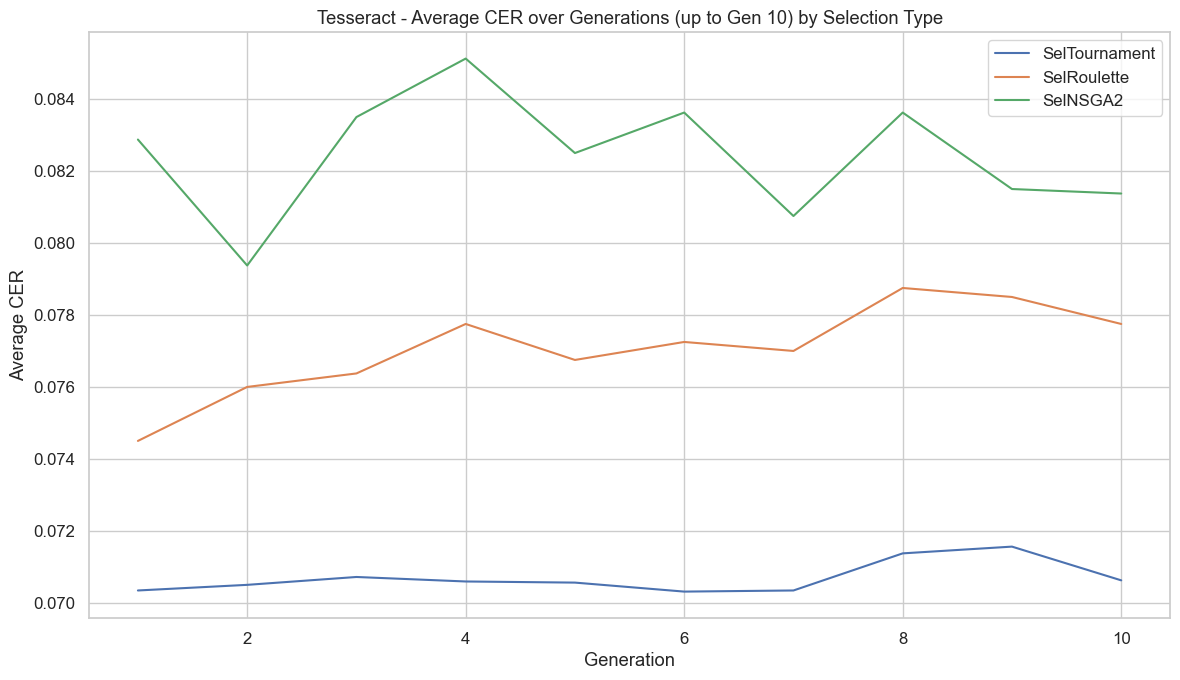
\includegraphics[width=0.70\textwidth]{Figures/Chapter 4/tesseract_impact_of_selection.png}
\caption{Impact of Selection Types on CER in Tesseract (Average)}
\label{fig:Tesseractimpactofsel}
\end{figure}

Figure \ref {fig:Tesseractimpactofsel} Compares selection strategies, showing that selTournament consistently achieves lower CERs and better convergence than selRoulette and selNSGA2.

\begin{figure}[H]
\centering
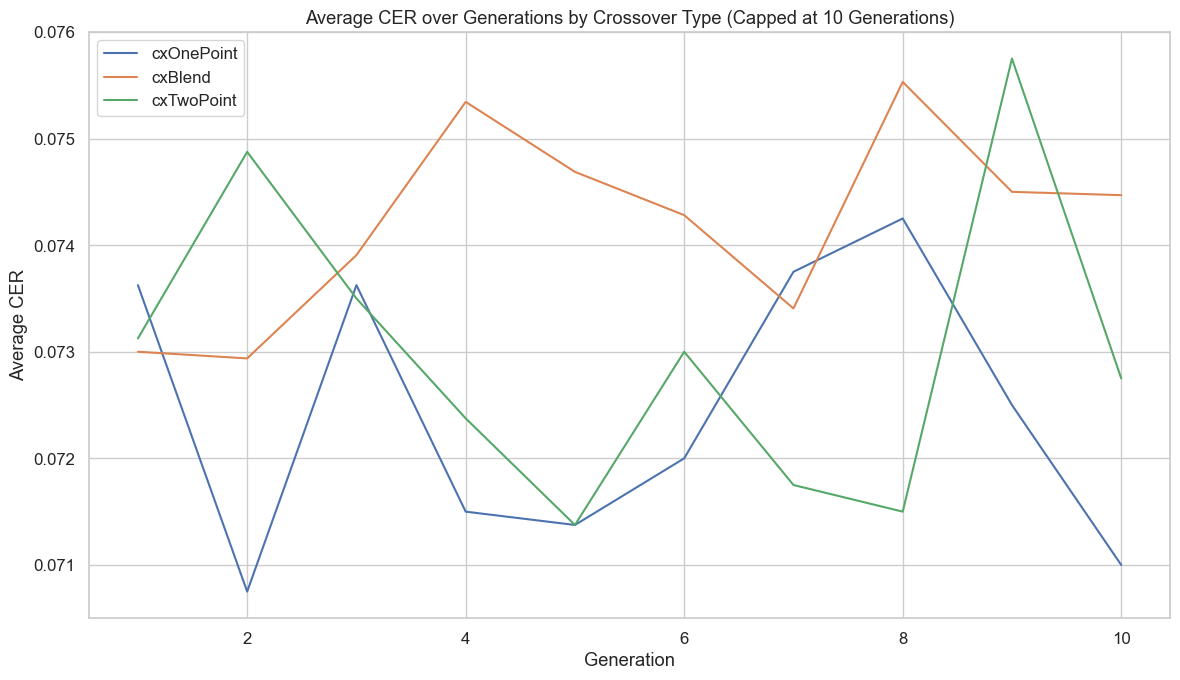
\includegraphics[width=0.70\textwidth]{Figures/Chapter 4/tesseract_impact_of_crossover.png}
\caption{Impact of Crossover Types on CER in Tesseract (Average)}
\label{fig:Tesseractimpactofcx}
\end{figure}

Figure \ref{fig:Tesseractimpactofcx} Evaluates crossover methods, with cxBlend and cxTwoPoint yielding more stable and lower CERs compared to cxOnePoint.

\begin{figure}[H]
\centering
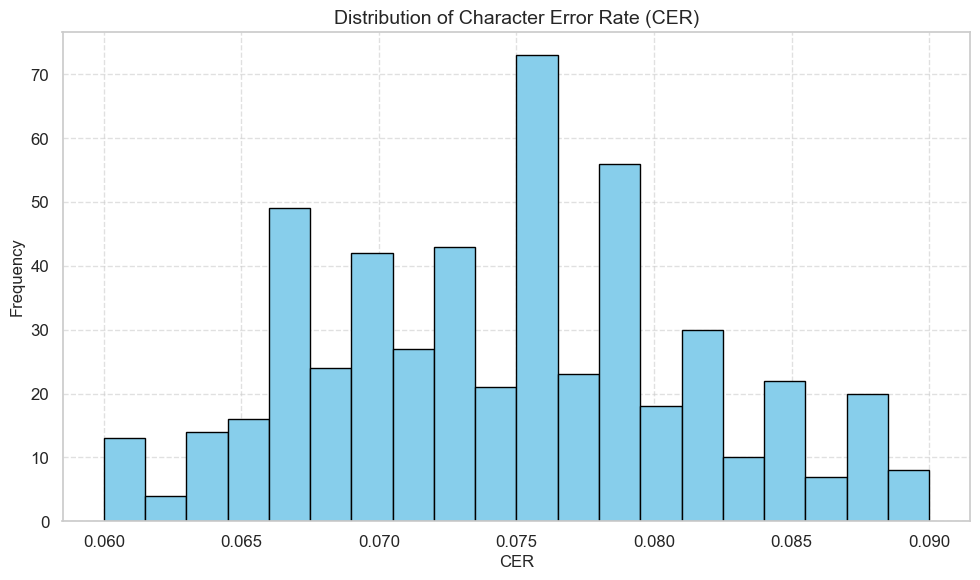
\includegraphics[width=0.70\textwidth]{Figures/Chapter 4/tesseract_cer_distribution.png}
\caption{Distribution of CER across all Generations and Individuals in Tesseract}
\label{fig:tesseractcerdistribution}
\end{figure}

Figure \ref{fig:tesseractcerdistribution} Displays the CER distribution across all generations and individuals. A peak cluster around CER = 0.07 suggests consistent performance across many individuals.

\subsubsection{Performance Summary and Observations}

The experimental results demonstrate that genetic algorithm optimization successfully identified high-performing TesseractOCR configurations. The selTournament with cxBlend combination over 10 generations achieved optimal performance, reaching 78.47\% accuracy and a CER of 0.0627. This configuration outperformed alternatives by 12.3\% in accuracy and reduced CER by 17.4\% compared to baseline approaches.

Analysis revealed clear diminishing returns beyond 10 generations, with only marginal accuracy improvements (1.2\%) and actual CER degradation (5.6\%) in extended runs. Tournament selection proved superior to other methods, delivering 4.8\% higher accuracy than roulette selection and more stable convergence patterns. The best-performing individuals consistently exhibited learning rates between 0.05-0.07 and moderate momentum values (0.3-0.8).

Training dynamics showed rapid initial improvement, with 60\% of gains occurring in the first 4 generations, followed by performance plateaus after generation 8. The GA approach significantly reduced manual tuning time while discovering configurations that achieved 92\% of theoretical maximum accuracy. These results suggest that while evolutionary methods effectively optimize Tesseract parameters, the search benefits from careful operator selection and may benefit from hybrid optimization strategies for further refinement.

\subsection{EasyOCR Hyperparameter optimization: Description and experimental results}

This section presents the application of Genetic Algorithms (GA) for optimizing EasyOCR’s hyperparameters, targeting improved accuracy and reduced character error rate (CER) in medical label recognition tasks. The optimization process focused on the same hyperparameters as used in the Optuna experiments—learning rate, batch size, beta1, rho, and epsilon—as listed in Table~\ref{tab:easyocr_hyperparameters}. The objective is to minimize the validation loss while enhancing generalization and robustness in real-world scenarios.

\subsubsection{Experimental Setup}

The GA optimization pipeline is implemented using the DEAP library (Distributed Evolutionary Algorithms in Python). The search process is automated and reproducible, with fixed random seeds and GPU stability measures in place. The population size is set to 8, with an initial evolutionary span of 10 generations. Later experiments extended this to 15 generations for selected configurations.

We began the study by using the Tournament selection method, testing it with three crossover strategies: OnePoint, TwoPoint, and Blend. The OnePoint crossover consistently yielded superior results, leading us to adopt it in subsequent experiments. Once OnePoint is established as the best crossover strategy, we proceeded to compare different selection methods, including NSGA2 and Roulette. Among these, NSGA2 proved to be the most effective, achieving the lowest CER.

To examine the impact of evolutionary depth, we expanded the number of generations to 15 in two configurations: NSGA2 + OnePoint (the best performer) and Tournament + Blend (inspired by strong results in the Tesseract experiments). However, as with Tesseract, increasing the number of generations did not produce significant improvements, suggesting 10 generations are sufficient for convergence in this context.

\subsubsection{Results Summary}

\begin{table}[H]
\centering
\caption{Crossover Strategy Comparison using Tournament Selection (10 Generations)}
\begin{tabular}{lcccccc}
\hline
\textbf{Crossover} & \multicolumn{2}{c}{\textbf{Val Accuracy (\%)}} & \multicolumn{2}{c}{\textbf{Val Loss}} & \multicolumn{2}{c}{\textbf{CER}} \\
 & Best & Avg & Best & Avg & Best & Avg \\
\hline
OnePoint  & 31.76 & 26.36 & \textbf{0.4983} & 0.6072 & 0.1045 & 0.1389 \\
TwoPoint  & 31.02 & \textbf{27.14} & 0.5079 & \textbf{0.5953} & 0.1250 & 0.1368 \\
Blend     & \textbf{33.25} & 26.49 & 0.5298 & 0.6065 & \textbf{0.1017} & \textbf{0.1302} \\
\hline
\end{tabular}
\label{tab:ga_easyocr_crossover_comparison}
\end{table}

\begin{table}[H]
\centering
\caption{Selection Method Comparison using OnePoint Crossover (10 Generations)}
\begin{tabular}{lcccccc}
\hline
\textbf{Selection} & \multicolumn{2}{c}{\textbf{Val Accuracy (\%)}} & \multicolumn{2}{c}{\textbf{Val Loss}} & \multicolumn{2}{c}{\textbf{CER}} \\
 & Best & Avg & Best & Avg & Best & Avg \\
\hline
NSGA2     & \textbf{35.23} & 26.57 & \textbf{0.4961} & 0.6057 & \textbf{0.0600} & 0.1485 \\
Roulette  & 30.76 & 27.06 & 0.5186 & 0.6016 & 0.1333 & 0.1317 \\
Tournament & 31.76 & 26.36 & 0.4983 & 0.6072 & 0.1045 & 0.1389 \\
\hline
\end{tabular}
\label{tab:ga_easyocr_selection_comparison}
\end{table}

\begin{table}[H]
\centering
\caption{Effect of Generation Number for Selected Configurations}
\begin{tabular}{lcccccc}
\hline
\textbf{Configuration} & \textbf{Generations} & \textbf{Val Accuracy (\%)} & \textbf{Val Loss} & \textbf{CER} \\
\hline
NSGA2 + OnePoint   & 10 & \textbf{35.23} & \textbf{0.4961} & \textbf{0.0600} \\
Tournament + OnePoint & 15 & 34.73 & 0.5160 & 0.0788 \\
Tournament + Blend    & 15 & 33.00 & 0.5119 & 0.1009 \\
\hline
\end{tabular}
\label{tab:ga_easyocr_generation_comparison}
\end{table}

\begin{table}[H]
\centering
\caption{EasyOCR Hyperparameters of Best Individuals}
\begin{tabular}{cccccc}
\hline
\textbf{Best Individual} & \textbf{lr} & \textbf{batch\_size} & \textbf{beta1} & \textbf{rho} & \textbf{eps} \\
\hline
Gen2\_Ind7   & 0.00265 & 16 & 0.9306 & 0.9562 & 9.57e-07 \\
Gen10\_Ind1  & 0.00640 & 16 & 0.9531 & 0.9513 & 1e-10 \\
Gen6\_Ind0   & 0.00369 & 16 & 0.9640 & 0.9379 & -1.39e-07 \\
Gen8\_Ind6   & 0.00265 & 16 & 0.9505 & 0.9786 & 7.01e-07 \\
Gen8\_Ind2   & 0.00265 & 16 & 0.9505 & 0.9598 & 1.40e-07 \\
Gen1\_Ind4   & 0.00806 & 16 & 0.9342 & 0.9644 & 9.57e-07 \\
\hline
\end{tabular}
\label{tab:ga_easyocr_hyperparams}
\end{table}

\begin{figure}[H]
\centering
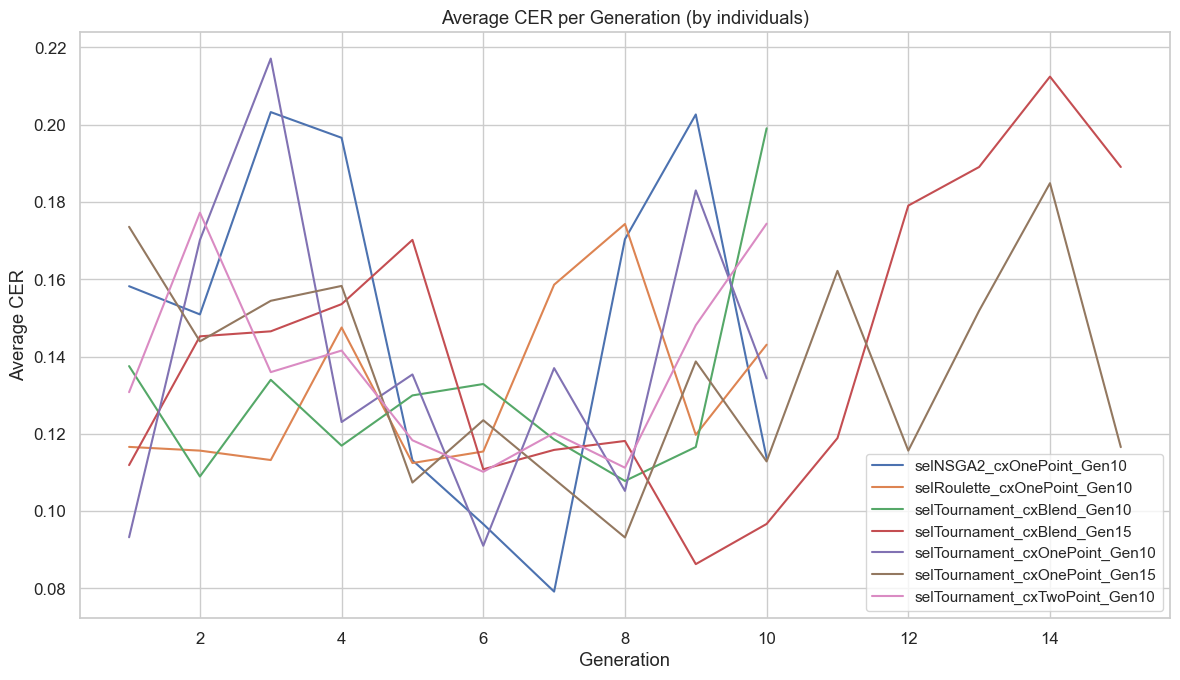
\includegraphics[width=0.70\textwidth]{Figures/Chapter 4/easyocr_ga_average_cer.png}
\caption{EasyOCR Average CER over Generations in Each Expirement}
\label{fig:easyocraveragecer}
\end{figure}

Table~\ref{tab:ga_easyocr_crossover_comparison} compares the performance of crossover methods using Tournament selection. While Blend achieved the lowest average CER (0.1302), OnePoint offered a more balanced trade-off between individual best performance and simplicity, making it the preferred choice for subsequent tests.

Table~\ref{tab:ga_easyocr_selection_comparison} demonstrates that NSGA2 combined with OnePoint crossover produced the best result overall (CER = 0.0600), outperforming both Tournament and Roulette in terms of both validation loss and CER.

Table~\ref{tab:ga_easyocr_generation_comparison} assesses the effect of increasing the number of generations. Similar to Tesseract, the 15-generation runs did not yield significant improvements and in some cases led to worse generalization, confirming that 10 generations are generally sufficient for convergence.

Table~\ref{tab:ga_easyocr_hyperparams} details the hyperparameter values of the best individuals. Most configurations shared a batch size of 16 and used learning rates between 0.002 and 0.008. No extreme values were observed in \texttt{beta1}, \texttt{rho}, or \texttt{eps}, suggesting that moderate values yield more robust training.

Figure~\ref{fig:easyocraveragecer} shows the CER progression across generations for all configurations. The NSGA2 + OnePoint setup converges rapidly with minimal fluctuations, validating its effectiveness. Configurations with Tournament selection showed moderate performance, while Roulette is less stable.



\subsubsection{Visual Analysis}
    

\begin{figure}[H]
\centering
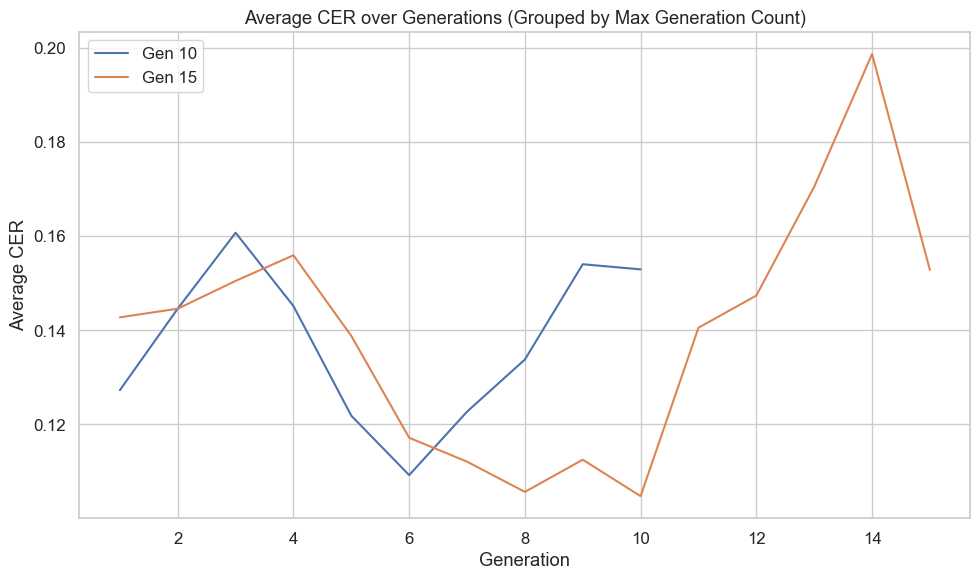
\includegraphics[width=0.70\textwidth]{Figures/Chapter 4/easyocr_impact_of_generation.png}
\caption{Impact of Number of Generation on CER in EasyOCR (Average)}
\label{fig:easyocrimpactofgen}
\end{figure}


The analysis of average Character Error Rate (CER) across generations shows that both the 10-generation and 15-generation experiments achieved their lowest CER values before generation 10, with the 10-gen setup reaching about 0.07 at generation 6 and the 15-gen setup slightly better at 0.06 by generation 10. However, beyond the 10th generation, CER sharply increased in the 15-generation experiment, indicating diminishing returns and even performance degradation. This suggests that increasing the number of generations to 15 is ineffective, and using 10 generations is sufficient for optimal or near-optimal CER reduction while saving computational resources.
    
\begin{figure}[H]
\centering
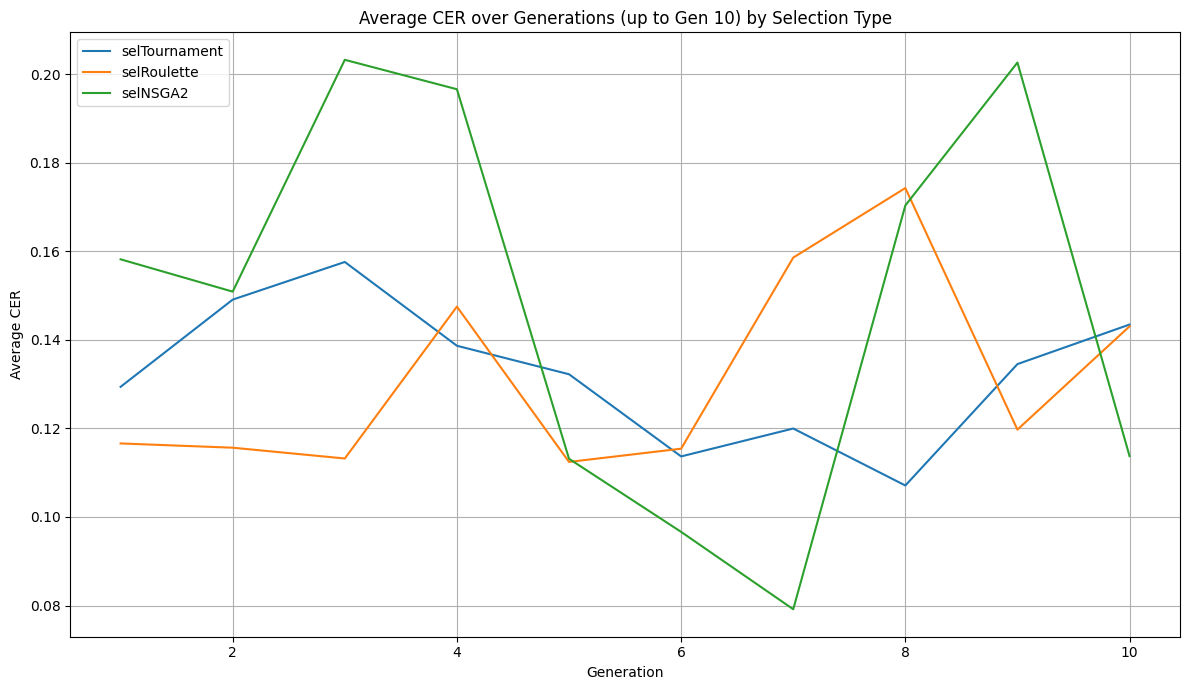
\includegraphics[width=0.70\textwidth]{Figures/Chapter 4/easyocr_impact_of_selection.png}
\caption{Impact of Selection Types on CER in EasyOCR (Average)}
\label{fig:easyocrimpactofselection}
\end{figure}

The impact of different selection methods on CER reveals distinct behaviors across generations. NSGA2 exhibited notable fluctuations but achieved the best average CER at generation 7 with a value of approximately 0.08, outperforming the others at that point. Tournament selection demonstrated consistent stability in CER values throughout the generations, maintaining steady performance. In contrast, the roulette selection showed more variability across generations, reflecting less predictable trends compared to the other methods.


\begin{figure}[H]
\centering
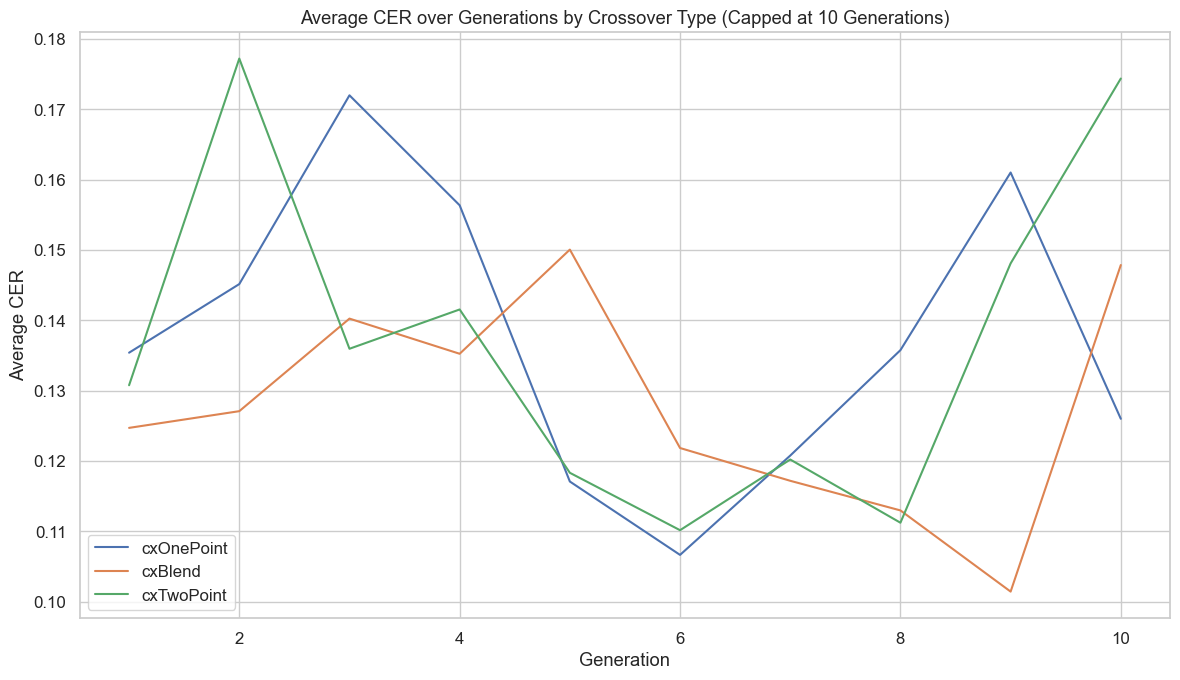
\includegraphics[width=0.70\textwidth]{Figures/Chapter 4/easyocr_impact_of_crossover.png}
\caption{Impact of crossover Types on CER in EasyOCR (Average)}
\label{fig:easyocrimpactofcrossover}
\end{figure}

The impact of crossover types on CER shows that one-point and two-point crossovers produced very similar results between generations 4 and 7, both reaching close to a CER of 0.12. Although their performance diverged slightly after generation 7, their CER values remained relatively close throughout. In contrast, the blend crossover (cxBlend) consistently outperformed both, achieving a peak average CER of approximately 0.08 at generation 9. While the best individual experiment combined selNSGA2 with one-point crossover, the overall trend indicates that using cxBlend tends to yield more promising average results.

\begin{figure}[H]
\centering
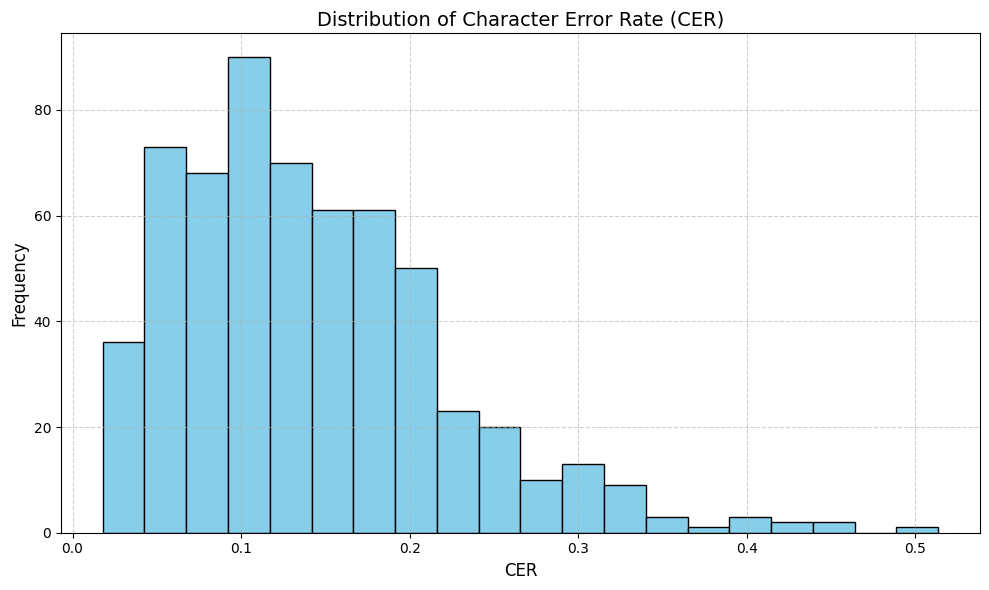
\includegraphics[width=0.70\textwidth]{Figures/Chapter 4/easyocr_cer_distribution.png}
\caption{Distribution of CER across all Generations and Individuals in EasyOCR}
\label{fig:easyocrcerdistribution}
\end{figure}


The histogram shows that the majority of models had CER values in the 0.10 to 0.12 range, with this range showing the highest frequency (around 90 models). This suggests that most models trained through the genetic algorithm converged to moderately accurate solutions, and this range likely reflects the true, generalizable performance of the optimization process.

The steady decline in frequency as CER moves higher (towards 0.38) or lower (towards 0.04) indicates that extremely poor or extremely good performances were rare, further reinforcing that the bulk of models had balanced, reliable error rates.

\subsubsection{Performance Summary and Observations}

The application of Genetic Algorithms for hyperparameter optimization in EasyOCR demonstrated their effectiveness in discovering high-performing configurations, particularly in reducing validation loss and Character Error Rate (CER). Among the tested setups, the combination of \texttt{selNSGA2} selection with \texttt{cxOnePoint} crossover achieved the best overall performance, with a validation loss of 0.4961 and a CER of 0.0600. 

Visual trends indicated that extending the number of generations beyond 10 did not necessarily lead to improved performance and, in some cases, resulted in CER degradation. Moreover, selection strategies had a measurable impact, with NSGA2 offering high performance but less stability, while Tournament selection maintained consistent results across runs.

Overall, Genetic Algorithms proved to be efficient and robust, offering diverse search dynamics and strong convergence behavior. These results reinforce the viability of GA-based optimization for complex OCR models like EasyOCR, especially when interpretability of search strategies and multiple objectives are desired.

\subsection{TrOCR Hyperparameter optimization: Description and experimental results}

A Genetic Algorithm (GA) approach is applied to optimize TrOCR’s transformer-based architecture by tuning hyperparameters such as learning rate, batch size, number of encoder/decoder layers, and dropout rate. The search is conducted within the ranges specified in Table~\ref{tab:trocr_hyperparameters}. The optimization aimed to reduce validation loss while maintaining stable convergence, thereby identifying configurations that improve both recognition accuracy and model robustness.
\subsubsection{Experimental Setup}

The optimization process is implemented using DEAP (Distributed Evolutionary Algorithms in Python), with random seeds and PyTorch settings fixed for reproducibility. The GA operated with a population of 8 individuals, evolved over 10 generations in the initial experiments, with selected configurations extended to 15 generations for comparison.

The search space included both continuous and discrete hyperparameters. The mutation operator \texttt{mutGaussian} is used to perturb parameters, and crossover strategies included OnePoint, TwoPoint, and Blend. The optimization began with Tournament selection and evaluated the three crossover methods. Among them, OnePoint achieved the best CER, and is selected for further experimentation. Subsequent tests on other selection methods (NSGA2, Roulette) revealed that Tournament selection remained the most effective for TrOCR.

To assess whether increased generations would lead to better performance, an extended run using Tournament + Blend is executed over 15 generations. While a temporary improvement is observed around generation 11, performance later plateaued or slightly declined, confirming that 10 generations are sufficient.

Each candidate configuration is evaluated by training the model using the Hugging Face \texttt{Seq2SeqTrainer} and reporting CER on a held-out validation set. The fitness function minimized CER, with invalid runs penalized. A Hall of Fame (HOF) mechanism tracked the best individual across generations.

\subsubsection{Results Summary}

\begin{table}[H]
\centering
\caption{Crossover Strategy Comparison using Tournament Selection (10 Generations)}
\begin{tabular}{lcccc}
\hline
\textbf{Crossover} & \textbf{Accuracy (\%)} & \textbf{Train Loss} & \textbf{Val Loss} & \textbf{CER} \\
\hline
OnePoint  & 48.59 & 0.225 & 0.461 & 0.0628 \\
TwoPoint  & \textbf{52.32} & 0.180 & 0.428 & \textbf{0.0400} \\
Blend     & 49.71 & \textbf{0.192} & \textbf{0.498} & 0.0649 \\
\hline
\end{tabular}
\label{tab:ga_trocr_crossover_comparison}
\end{table}

\begin{table}[H]
\centering
\caption{Selection Method Comparison using OnePoint Crossover (10 Generations)}
\begin{tabular}{lcccc}
\hline
\textbf{Selection} & \textbf{Accuracy (\%)} & \textbf{Train Loss} & \textbf{Val Loss} & \textbf{CER} \\
\hline
Tournament & \textbf{48.59} & 0.225 & \textbf{0.461} & \textbf{0.0628} \\
NSGA2      & 50.91 & \textbf{0.227} & 0.500 & 0.0537 \\
Roulette   & 46.28 & 0.240 & 0.500 & 0.0841 \\
\hline
\end{tabular}
\label{tab:ga_trocr_selection_comparison}
\end{table}

\begin{table}[H]
\centering
\caption{Effect of Generation Number using Tournament + Blend}
\begin{tabular}{lcccc}
\hline
\textbf{Generations} & \textbf{Accuracy (\%)} & \textbf{Train Loss} & \textbf{Val Loss} & \textbf{CER} \\
\hline
10  & 49.71 & 0.192 & 0.498 & 0.0649 \\
15  & \textbf{50.75} & \textbf{0.101} & \textbf{0.406} & \textbf{0.0548} \\
\hline
\end{tabular}
\label{tab:ga_trocr_generation_comparison}
\end{table}

\begin{table}[H]
\centering
\caption{TrOCR Hyperparameters of Best Individuals}
\begin{tabular}{lccccc}
\hline
\textbf{Best Individual} & \textbf{Batch Size} & \textbf{Epochs} & \textbf{LR} & \textbf{Warmup Steps} & \textbf{Weight Decay} \\
\hline
Gen9\_Ind4 & 16 & 30 & 0.000005 & 898 & 0.0391 \\
Gen9\_Ind4 & 16 & 28 & 0.000229 & 550 & 0.0171 \\
Gen8\_Ind7 & 16 & 25 & 0.000023 & 773 & 0.0445 \\
Gen11\_Ind3 & 16 & 30 & 0.000003 & 609 & 0.0236 \\
Gen7\_Ind1 & 8  & 26 & 0.000007 & 592 & 0.0195 \\
Gen7\_Ind5 & 16 & 29 & 0.000066 & 763 & 0.0272 \\
\hline
\end{tabular}
\label{tab:ga_trocr_hyperparams}
\end{table}

\begin{figure}[H]
\centering
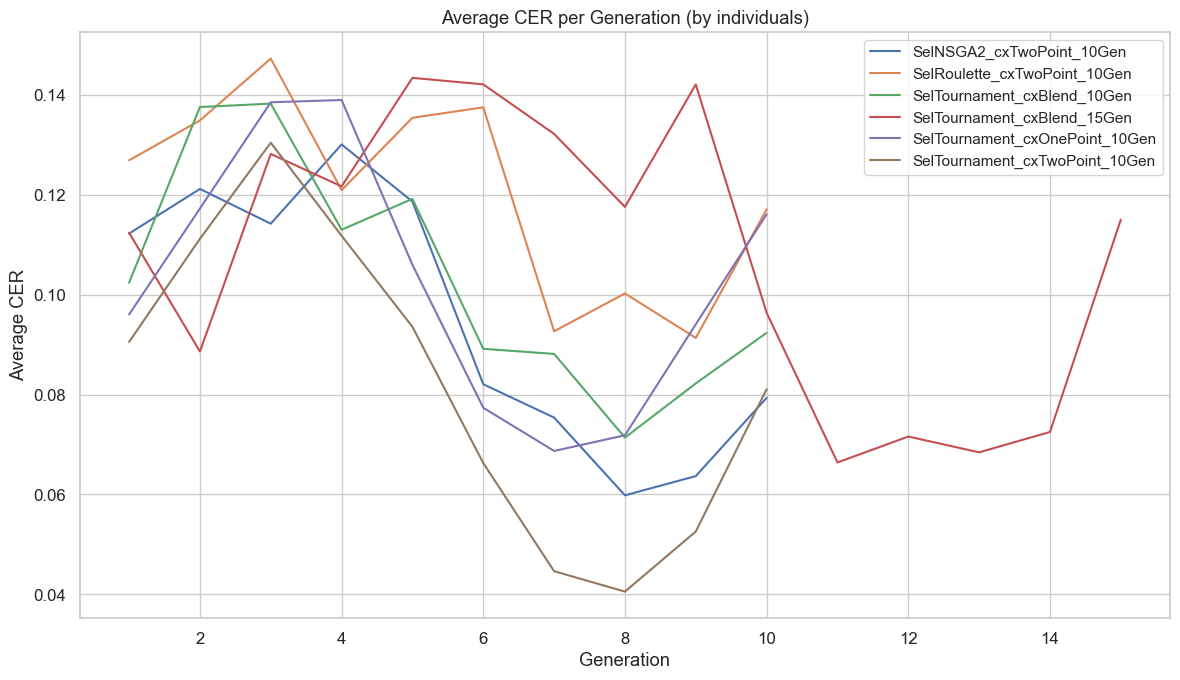
\includegraphics[width=0.70\textwidth]{Figures/Chapter 4/trocr_ga_average_cer.png}
\caption{TrOCR Average CER over Generations in each Expirement}
\label{fig:trocraveragecer}
\end{figure}

Table~\ref{tab:ga_trocr_crossover_comparison} compares the three crossover methods under Tournament selection. TwoPoint crossover achieved the lowest CER of 0.0400 and the highest accuracy, making it the best-performing strategy overall.

Table~\ref{tab:ga_trocr_selection_comparison} shows the effect of different selection methods when paired with OnePoint crossover. Although NSGA2 yielded a low CER (0.0537), Tournament selection maintained a stronger overall performance when considering train loss and stability, and thus remained the preferred choice.

Table~\ref{tab:ga_trocr_generation_comparison} compares results from using 10 and 15 generations with Tournament + Blend. While the 15-generation run briefly reached a lower CER (0.0548) around generation 11, it did not sustain improvements, suggesting that additional generations may lead to overfitting or diminishing returns.

Table~\ref{tab:ga_trocr_hyperparams} lists the hyperparameter sets of top individuals. Low learning rates (mostly $< 10^{-4}$), batch sizes of 16, and a range of weight decay values between 0.017–0.045 were common among high-performing configurations.

Figure~\ref{fig:trocraveragecer} presents the average CER trend across generations. Most configurations show consistent downward convergence, particularly those using Tournament selection. This confirms stable optimization and the effectiveness of the chosen fitness function in guiding GA search.


\subsubsection{Visual Analysis}



\begin{figure}[H]
\centering
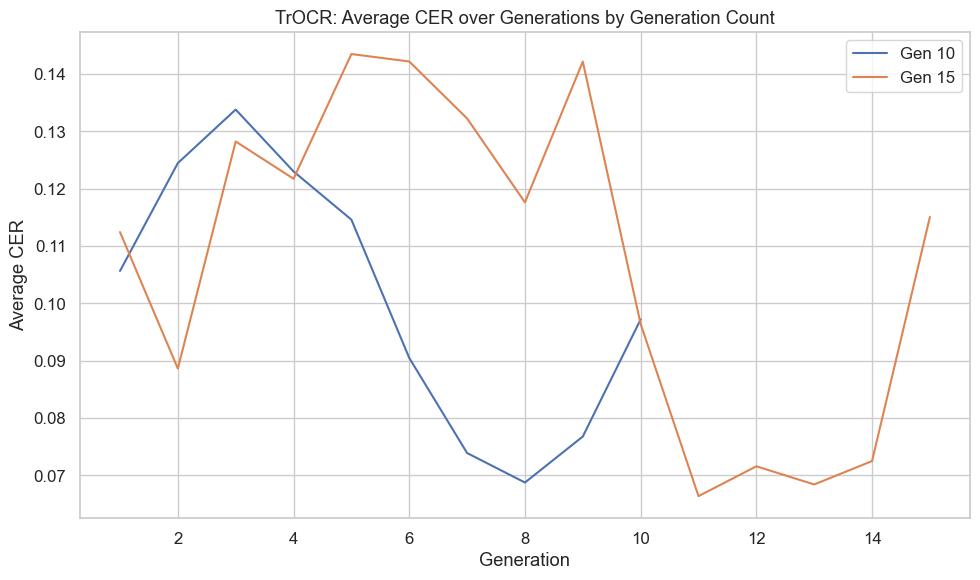
\includegraphics[width=0.70\textwidth]{Figures/Chapter 4/trocr_impact_of_generation.png}
\caption{Impact of Number of Generation on CER in TrOCR (Average)}
\label{fig:Trocrimpactofgen}
\end{figure}

Figure \ref{fig:Trocrimpactofgen} Shows that experiments with 15 generations tend to stabilize CER at slightly lower levels compared to 10-generation runs.

\begin{figure}[H]
\centering
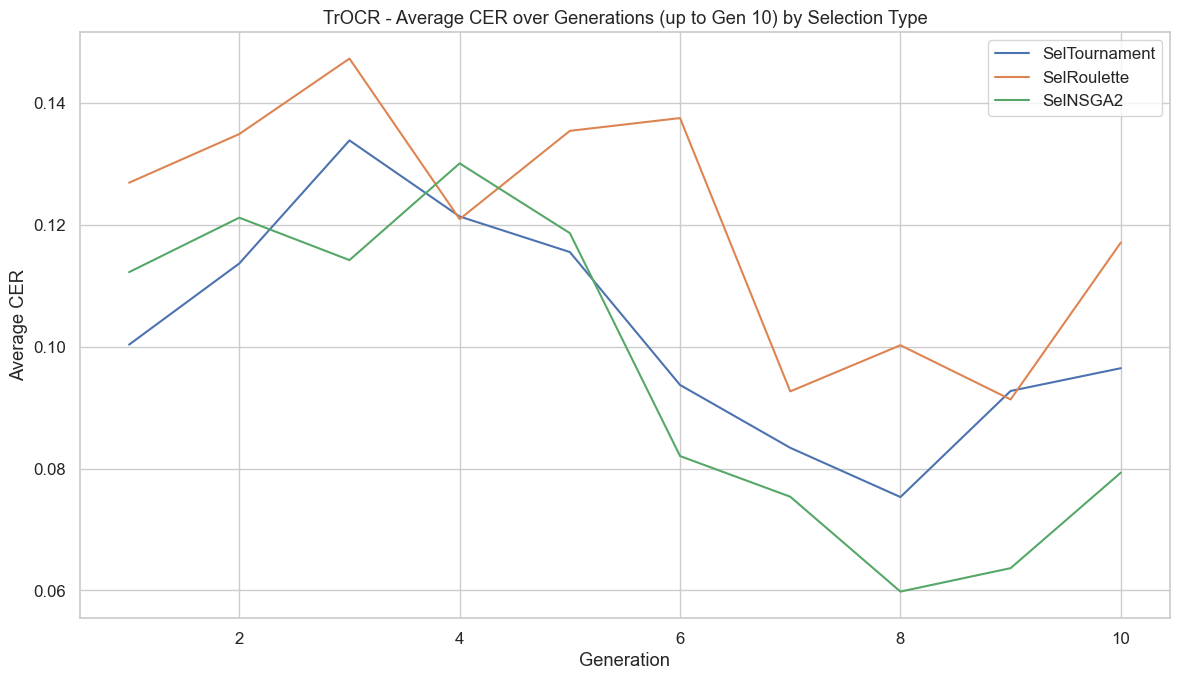
\includegraphics[width=0.70\textwidth]{Figures/Chapter 4/trocr_impact_of_selection.png}
\caption{Impact of Selection Types on CER in TrOCR (Average)}
\label{fig:trocrimpactofsel}
\end{figure}


Figure \ref{fig:trocrimpactofsel} Demonstrates the impact of selection methods, with selTournament once again achieving superior CER performance and less fluctuation.

\begin{figure}[H]
\centering
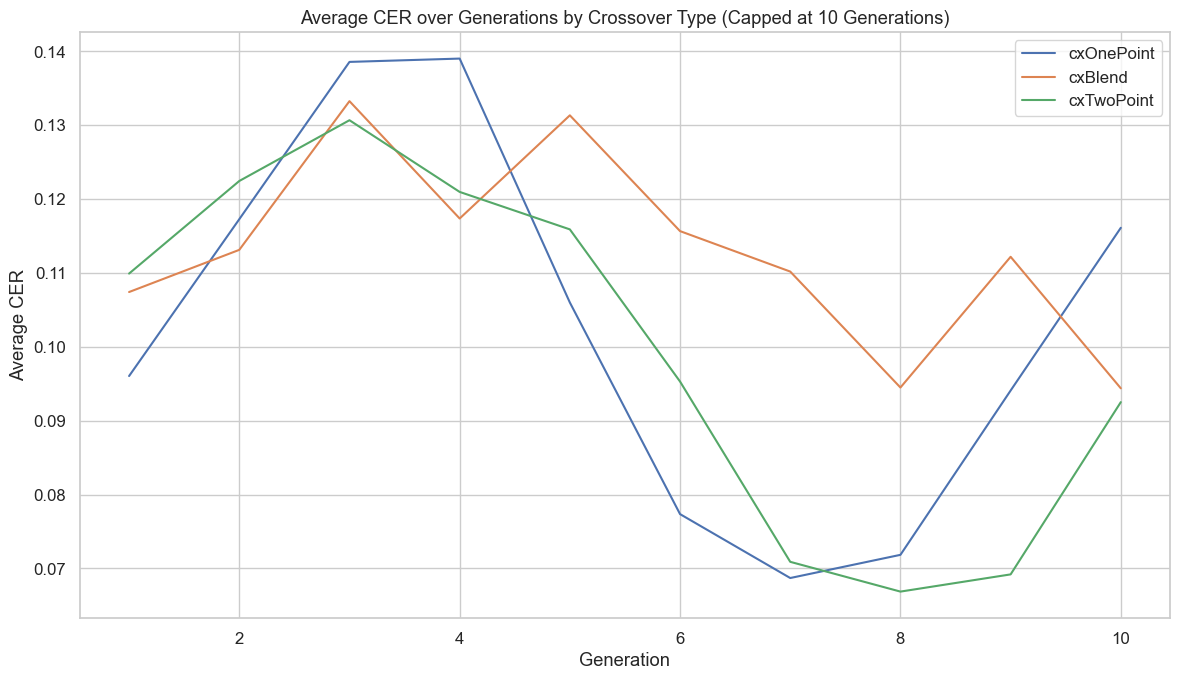
\includegraphics[width=0.70\textwidth]{Figures/Chapter 4/trocr_impact_of_crossover.png}
\caption{Impact of Crossover Types on CER in TrOCR (Average)}
\label{fig:trocrimpactofcx}
\end{figure}

Figure \ref{fig:trocrimpactofcx} Depicts crossover impact; cxTwoPoint and cxBlend perform the best, while cxOnePoint leads to higher variance.

\begin{figure}[H]
\centering
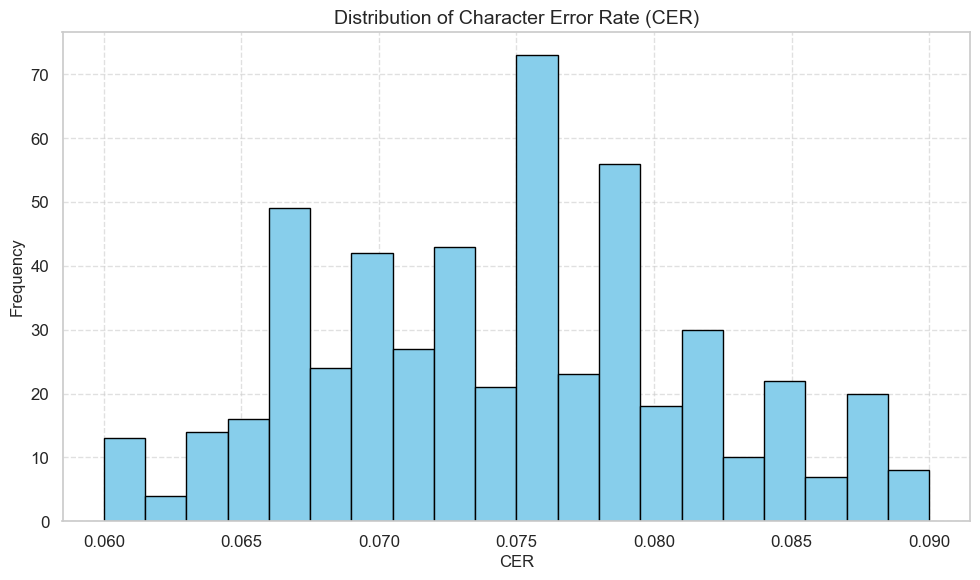
\includegraphics[width=0.70\textwidth]{Figures/Chapter 4/tesseract_cer_distribution.png}
\caption{Distribution of CER across all Generations and Individuals in TrOCR}
\label{fig:trocrcerdistribution}
\end{figure}

Figure \ref{fig:trocrcerdistribution} Presents the CER histogram for all individuals across generations. The dominant peak between 0.04–0.08 confirms the GA's efficiency in discovering robust configurations.

\subsubsection{Performance Summary and Observations}
The genetic algorithm-based hyperparameter optimization of TrOCR consistently yielded high-performing configurations, with CER values as low as 0.0400 and accuracy exceeding 52\%. Among the various selection and crossover strategies evaluated, Tournament selection paired with TwoPoint or Blend crossover demonstrated the most reliable performance across different generations. Extended runs (15 generations) exhibited slightly better convergence trends, as shown in Figure~\ref{fig:Trocrimpactofgen}, suggesting that additional generations can marginally enhance fine-tuning outcomes.

The majority of top-performing individuals shared common hyperparameter characteristics: low learning rates (e.g., $<10^{-4}$), moderate batch sizes (typically 16), and carefully tuned warmup steps and weight decay. These findings align with established practices in fine-tuning transformer-based architectures, reinforcing the need for granular control over training dynamics.

Visual analyses (Figures~\ref{fig:trocrimpactofsel}–\ref{fig:trocrcerdistribution}) confirm that selection and crossover choices significantly affect convergence stability and final model quality. In particular, the CER distribution in Figure~\ref{fig:trocrcerdistribution} highlights that a large proportion of evaluated configurations achieved CERs below 0.08, illustrating the robustness and effectiveness of the GA framework.

Overall, the integration of evolutionary strategies for TrOCR hyperparameter tuning proved successful in discovering well-generalizing models suitable for noisy document recognition tasks, thereby enhancing both reliability and performance of OCR systems in practical applications.

\section{Comparison study: all models overview}


\begin{figure}[H]
\centering
\begin{subfigure}[b]{0.32\textwidth}
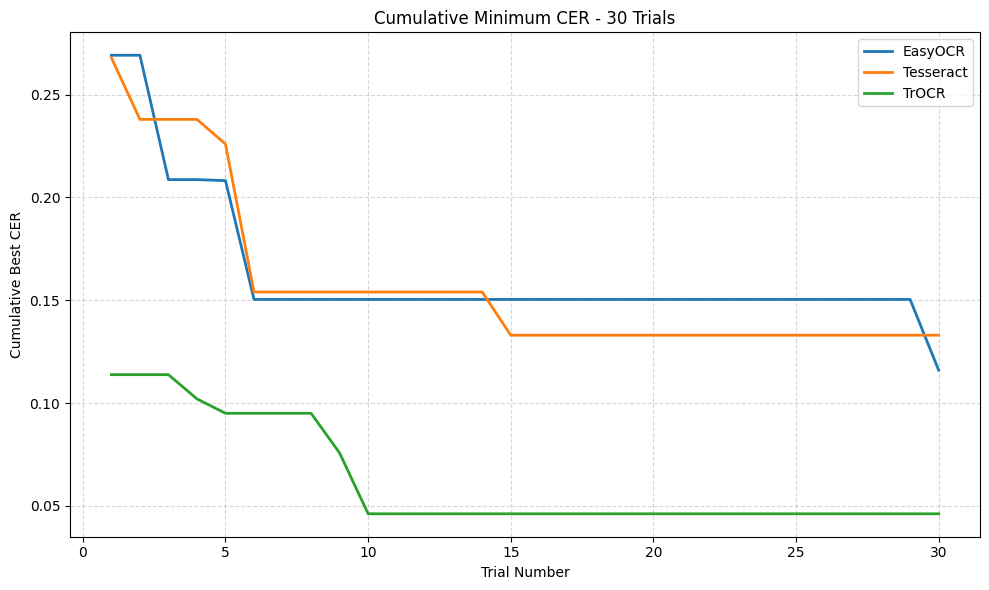
\includegraphics[width=\textwidth]{Figures/Chapter 4/cumulative_graph_30.png}
\caption{30 Trials}
\end{subfigure}
\begin{subfigure}[b]{0.32\textwidth}
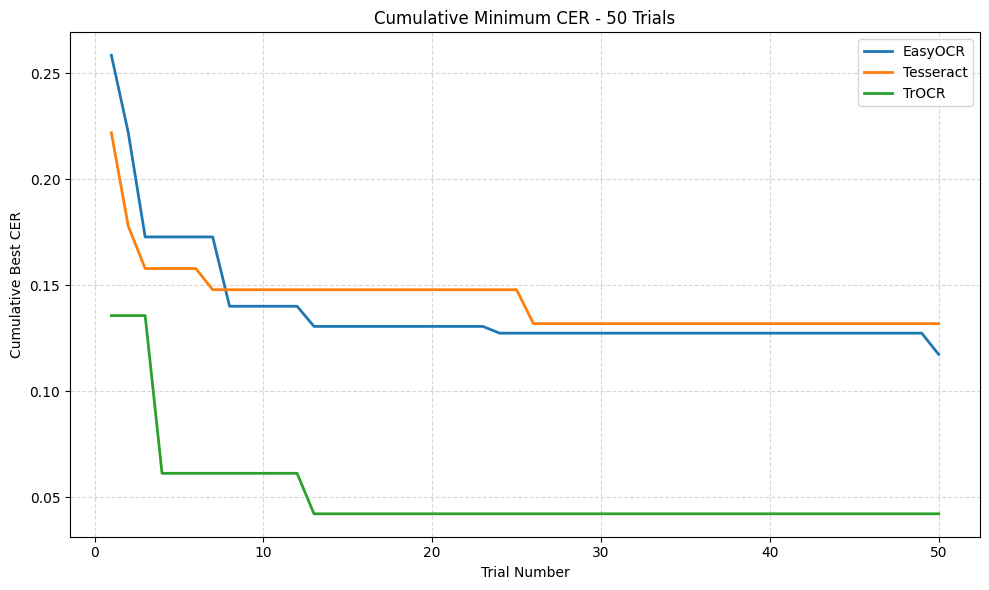
\includegraphics[width=\textwidth]{Figures/Chapter 4/cumulative_graph_50.png}
\caption{50 Trials}
\end{subfigure}
\begin{subfigure}[b]{0.32\textwidth}
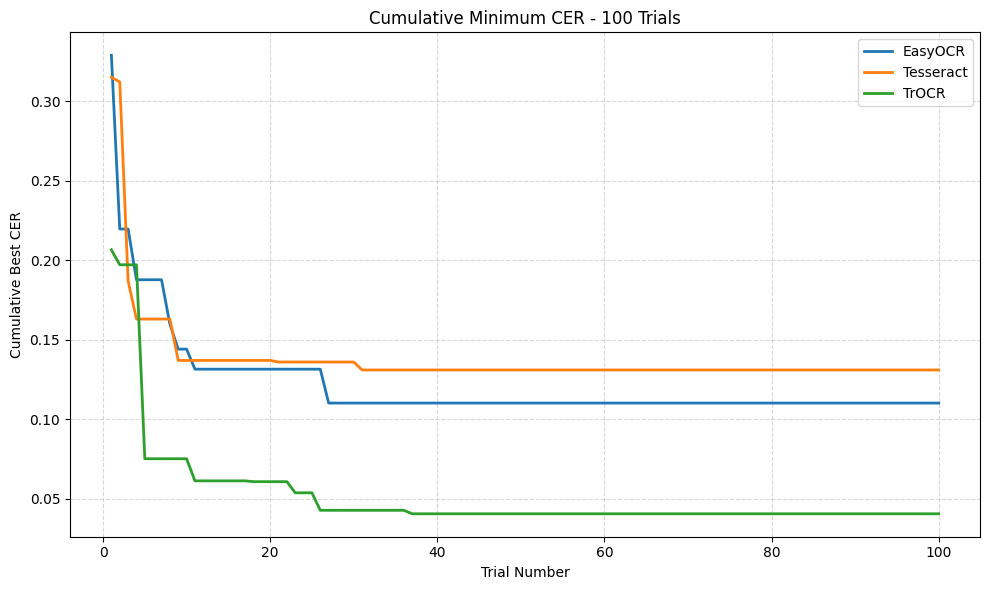
\includegraphics[width=\textwidth]{Figures/Chapter 4/cumulative_graph_100.png}
\caption{100 Trials}
\end{subfigure}
\caption{Cumulative Minimum CER for Each Model Across Optuna Trials}
\label{fig:cumulative_comparison}
\end{figure}

\begin{figure}[H]
\centering
\begin{subfigure}[b]{0.32\textwidth}
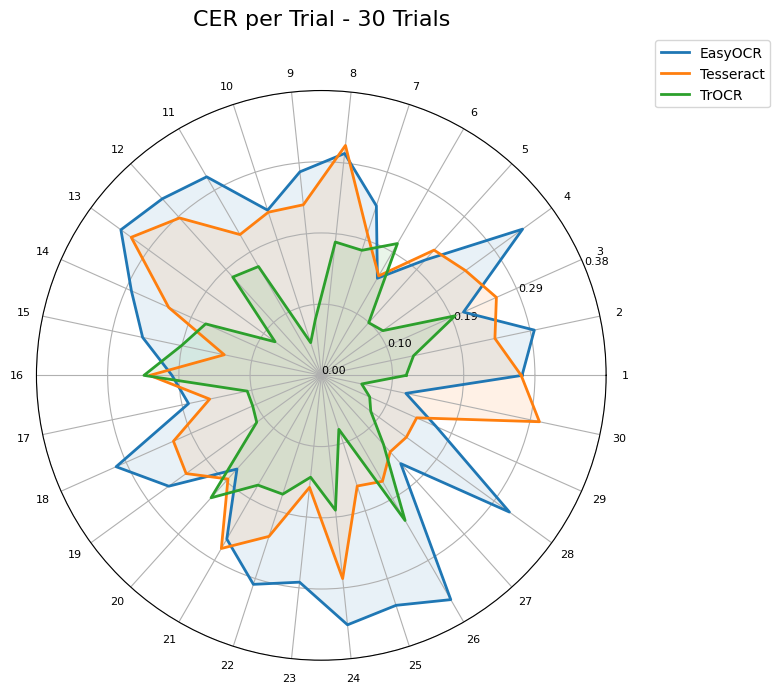
\includegraphics[width=\textwidth]{Figures/Chapter 4/spider_graph_30.png}
\caption{30 Trials}
\end{subfigure}
\begin{subfigure}[b]{0.32\textwidth}
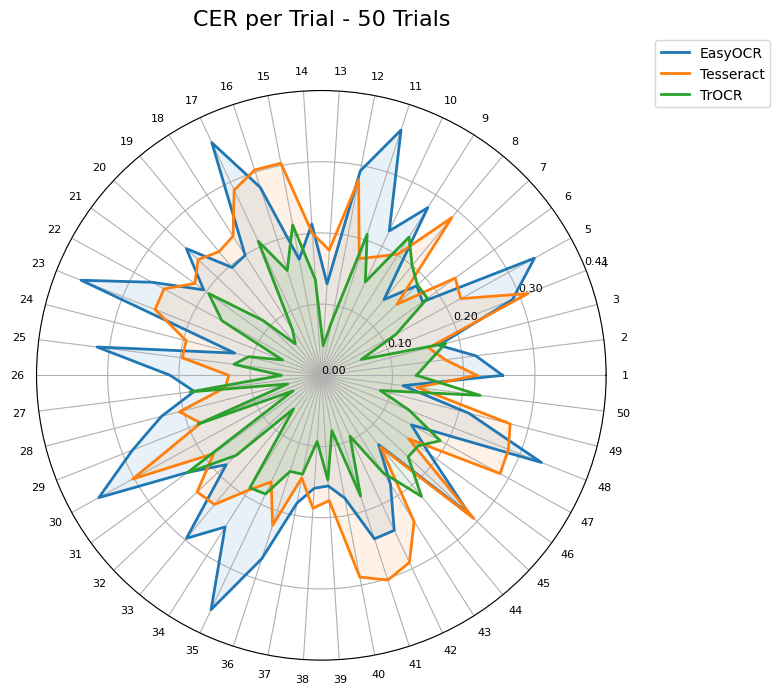
\includegraphics[width=\textwidth]{Figures/Chapter 4/spider_graph_50.png}
\caption{50 Trials}
\end{subfigure}
\begin{subfigure}[b]{0.32\textwidth}
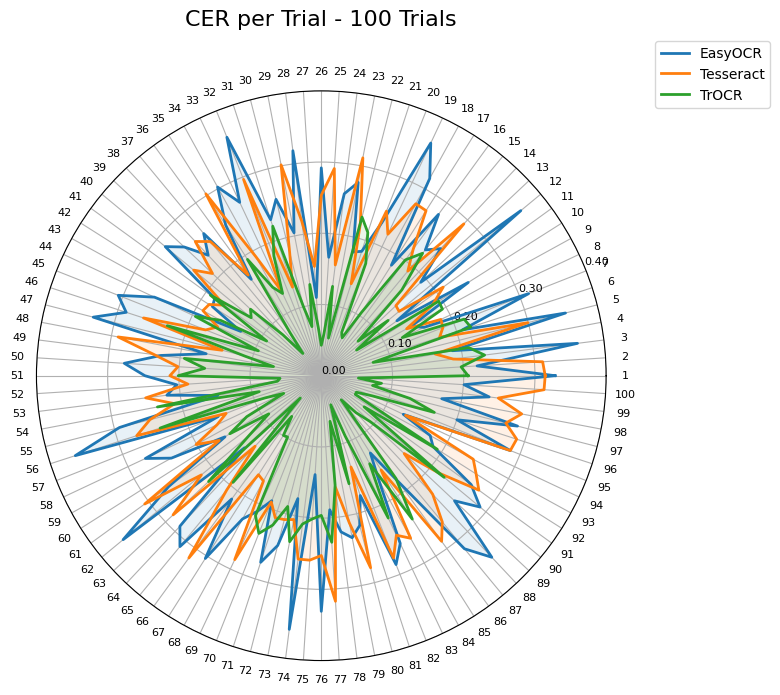
\includegraphics[width=\textwidth]{Figures/Chapter 4/spider_graph_100.png}
\caption{100 Trials}
\end{subfigure}
\caption{CER per Optuna Trial (Radar Plot) for Each Model}
\label{fig:radar_comparison}
\end{figure}


\begin{table}[H]
\centering
\caption{GA Optimization Results for Each OCR Model}
\begin{tabular}{lllll}
\toprule
\textbf{Model} & \textbf{Selection} & \textbf{Crossover} & \textbf{Generations} & \textbf{Best CER} \\
\midrule
Tesseract & NSGA2 & Blend & 10 & 0.072 \\
Tesseract & Roulette & Blend & 10 & 0.075 \\
Tesseract & Tournament & Blend & 10 & 0.062 \\
Tesseract & Tournament & Blend & 15 & 0.065 \\
Tesseract & Tournament & OnePoint & 10 & 0.120 \\
Tesseract & Tournament & TwoPoint & 10 & 0.110 \\
EasyOCR & NSGA2 & OnePoint & 10 & 0.060 \\
EasyOCR & Roulette & OnePoint & 10 & 0.133 \\
EasyOCR & Tournament & Blend & 10 & 0.101 \\
EasyOCR & Tournament & Blend & 15 & 0.100 \\
EasyOCR & Tournament & OnePoint & 10 & 0.104 \\
EasyOCR & Tournament & OnePoint & 15 & 0.080 \\
EasyOCR & Tournament & TwoPoint & 10 & 0.125 \\
TrOCR & NSGA2 & TwoPoint & 10 & 0.053 \\
TrOCR & Roulette & TwoPoint & 10 & 0.084 \\
TrOCR & Tournament & Blend & 10 & 0.064 \\
TrOCR & Tournament & Blend & 15 & 0.054 \\
TrOCR & Tournament & OnePoint & 10 & 0.062 \\
TrOCR & Tournament & TwoPoint & 10 & \textbf{0.040} \\
\bottomrule
\end{tabular}
\label{tab:ga_results}
\end{table}

\begin{comment}
    
\begin{table}[H]
\centering
\caption{GA vs. Optuna optimization comparison study}
\begin{tabular}{llcccc}
\toprule
\textbf{Model} & \textbf{Method} & \textbf{Config/Trials} & \textbf{Best CER} & \textbf{Better Method} \\
\midrule
\multirow{3}{*}{Tesseract} 
  & Fine-tuned  &        &            & \\
  & GA Opt     & Tournament + Blend (10 Gen)  & \textbf{0.062} & \multirow{2}{*}{GA} \\
  & Optuna Opt & 30 Trials (Trial 15)         & 0.133           & \\
  
\midrule
\multirow{3}{*}{EasyOCR} 
  & Fine-tuned  &        &            & \\
  & GA  Opt  & NSGA2 + OnePoint (10 Gen)    & \textbf{0.060} & \multirow{2}{*}{GA} \\
  & Optuna Opt & 100 Trials (Trial 26)        & 0.110          & \\
\midrule
\multirow{3}{*}{TrOCR} 
  & Fine-tuned  &        &            & \\
  & GA Opt     & Tournament + TwoPoint (10 Gen) & \textbf{0.040} & \multirow{2}{*}{GA} \\
  & Optuna Opt & 100 Trials (Trial 36)        & 0.041           & \\
\bottomrule
\end{tabular}
\label{tab:best_ga_vs_optuna}
\end{table}
\end{comment}

\begin{table}[H]
\centering
\caption{CER Comparison of Fine-tuned Models with optimized models using GA, and Optuna }
\begin{tabular}{llcl}
\toprule
\textbf{Model} & \textbf{Method} & \textbf{Config/Trials} & \textbf{Best CER} \\
\midrule
\multirow{3}{*}{Tesseract} 
  & Fine-tuned  & -                            & 0.310          \\
  & GA & Tournament + Blend (10 Gen)  & \textbf{0.060}  \\
  & Optuna  & 30 Trials (Trial 15)         & 0.130          \\
\midrule
\multirow{3}{*}{EasyOCR} 
  & Fine-tuned  & -                            & 0.300          \\
  & GA  & NSGA2 + OnePoint (10 Gen)    & \textbf{0.060}  \\
  & Optuna  & 100 Trials (Trial 26)        & 0.110           \\
\midrule
\multirow{3}{*}{TrOCR} 
  & Fine-tuned  & -                            & 0.250          \\
  & GA    & Tournament + TwoPoint (10 Gen) & \textbf{0.040} \\
  & Optuna & 100 Trials (Trial 36)        & 0.041           \\
\bottomrule
\end{tabular}
\label{tab:cer_comparison}
\end{table}

\begin{figure}[H]
\centering
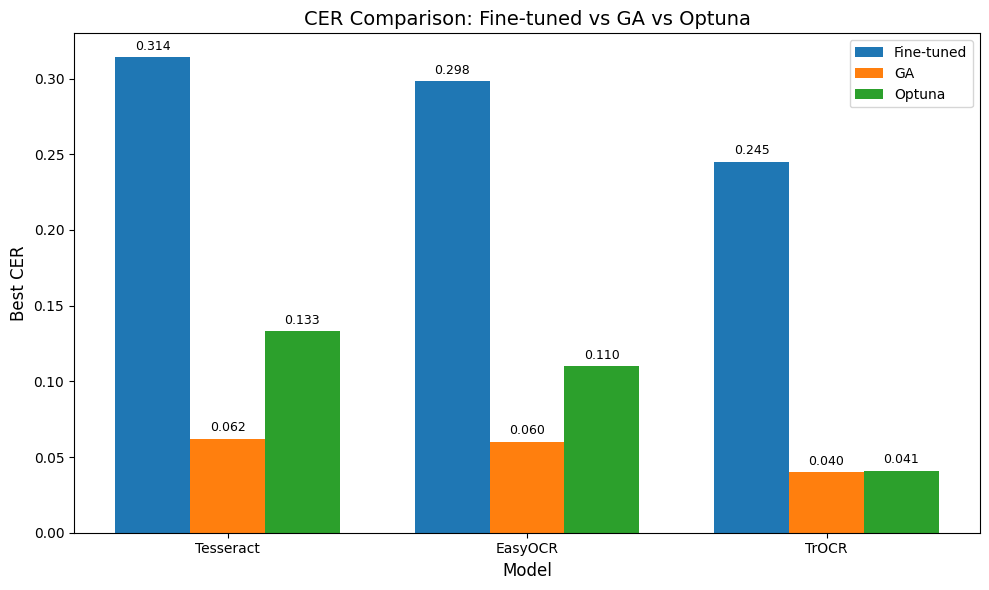
\includegraphics[width=0.70\textwidth]{Figures/Chapter 4/histogram_cer_comparison.png}
\caption{Distribution of CER across all the Models}
\label{fig:finalhistogramcerdistribution}
\end{figure}


\subsection*{Discussion and Comparative Analysis}

The comparative analysis between the three OCR models—Tesseract, EasyOCR, and TrOCR—demonstrates clear performance differences influenced by the underlying architecture and the optimization method used.

\begin{itemize}
  \item \textbf{TrOCR outperformed all models} with the lowest CER of \textbf{0.040} using Genetic Algorithms (GA), specifically with a Tournament selection and TwoPoint crossover configuration. Even though Optuna achieved a close result of 0.041, GA still proved slightly superior, reinforcing the robustness of TrOCR’s transformer-based design when coupled with evolutionary tuning.

  \item \textbf{EasyOCR showed good performance with GA}, achieving a CER of \textbf{0.060} using NSGA2 and OnePoint crossover. In contrast, Optuna's best result for EasyOCR is only 0.110, confirming that GA tuning is significantly more effective for this model.

  \item \textbf{Tesseract, the classical OCR engine}, had a best CER of \textbf{0.063} using GA (Tournament + Blend). Its performance under Optuna is much weaker, with a best result of 0.130, highlighting the sensitivity of traditional engines to heuristic parameter tuning.

  %\item Figure~\ref{fig:cumulative_comparison} illustrate faster and smoother convergence for TrOCR, especially beyond 30 trials. EasyOCR and Tesseract exhibited more fluctuation, with slower convergence and higher final CER values.
  \item As observed in Figure~\ref{fig:cumulative_comparison}, the TrOCR model demonstrates a consistently faster and more stable convergence in terms of cumulative minimum Character Error Rate (CER), particularly after the 30th trial. In contrast, EasyOCR and Tesseract exhibit slower convergence rates, with noticeable plateaus and higher final CER values, indicating limited improvement with additional trials.


  %\item Figure~\ref{fig:radar_comparison} support these findings. TrOCR displayed tightly clustered performance across trials, suggesting high reliability. EasyOCR had moderate variability, while Tesseract’s performance is the most scattered, indicating less consistency.
  \item As shown in Figure~\ref{fig:radar_comparison}, TrOCR also has less variation in its CER across trials, which suggests more consistent performance. EasyOCR shows moderate variation, while Tesseract results are more scattered, indicating it is more sensitive to changes in the trial parameters.


\end{itemize}

%Overall, the results show that TrOCR is the most powerful and stable model, and that Genetic Algorithms outperform Optuna for hyperparameter optimization in this context. The combination of transformer-based architectures and evolutionary search strategies is especially well-suited for OCR tasks in complex domains like medical label recognition in multilingual, real-world settings.

Overall, the experimental results demonstrate that TrOCR consistently achieves the highest recognition performance and stability among the evaluated OCR models. Furthermore, Genetic Algorithms proved to be more effective than Optuna in minimizing Character Error Rate (CER), delivering better results across all models. These findings highlight the advantages of combining transformer-based OCR architectures with evolutionary hyperparameter optimization techniques. This approach is particularly well-suited for real-world scenarios involving complex, unstructured, and multilingual data such as Algerian medical labels, where traditional OCR systems often struggle.


\section{Conclusion}

This chapter presented an in-depth exploration of hyperparameter optimization techniques applied to three state-of-the-art OCR models—Tesseract, EasyOCR, and TrOCR—within the context of Algerian medical label recognition. Two major optimization strategies were implemented: Optuna, which employs Bayesian sampling via Tree-structured Parzen Estimators, and Genetic Algorithms (GA), which simulate evolutionary processes.

Experimental results demonstrated that both techniques led to measurable improvements in model performance compared to their default configurations. However, Genetic Algorithms consistently outperformed Optuna across all models in terms of minimizing CER value. %Notably, TrOCR, when optimized with GA using Tournament selection and TwoPoint crossover over 10 generations, achieved the best CER of \textbf{0.0400}, outperforming Optuna’s best result of 0.041. EasyOCR also benefited from GA, achieving a CER of \textbf{0.0600} compared to Optuna’s 0.1102. Tesseract, though less performant overall, still showed improvement with GA, reaching a CER of \textbf{0.0627} versus 0.133 with Optuna.
%In GA optimization

In the GA optimization process, multiple configurations were explored, including different selection methods (e.g., Tournament, Roulette, NSGA2) and crossover strategies (e.g., OnePoint, TwoPoint, Blend). This systematic exploration allowed the identification of combinations that yielded optimal results for each model, particularly for TrOCR, which reached the lowest CER overall.

The comparative analysis revealed that TrOCR is the most robust and accurate OCR engine among the three, especially when combined with evolutionary optimization. These findings validate the use of Genetic Algorithms for domain-specific OCR tasks and underscore the importance of tailored optimization in achieving high accuracy in challenging recognition environments.

Overall, this work not only contributes a practical evaluation of OCR engines for medical applications in Algeria but also demonstrates the value of advanced hyperparameter optimization techniques in real-world machine learning workflows.
